% -*- TeX-engine: xetex;  -*-
\documentclass[
letterpaper, % Stock and paper size.
11pt, % Type size.
% article,
oneside, 
onecolumn, % Only one column of text on a page.
% openright, % Each chapter will start on a recto page.
% openleft, % Each chapter will start on a verso page.
openany, % A chapter may start on either a recto or verso page.
]{memoir}

%%% PACKAGES 
%%%------------------------------------------------------------------------------

%\usepackage[utf8]{inputenc} % Not needed with XeTeX
\usepackage[T1]{fontenc}    %
\usepackage[english]{babel} % English please
\usepackage[final]{microtype} % Less badboxes

%\usepackage{amsmath,amssymb,mathtools} % Math

\usepackage{newtxtext}
\usepackage{newtxmath}
%\usepackage{dutchcal} % For lower-case calligraphic
\usepackage{boondox-calo} % For lower-case calligraphic
\usepackage{pstricks,pst-node}
\usepackage{multido}
\usepackage{url}
\usepackage[small,bf]{caption}
%\usepackage[dvips]{graphicx} % Include figures
\usepackage{siunitx}
\usepackage{enumitem}
\usepackage{graphicx}
%%% PAGE LAYOUT 
%%%------------------------------------------------------------------------------

\setlrmarginsandblock{0.15\paperwidth}{*}{1} % Left and right margin
\setulmarginsandblock{0.2\paperwidth}{*}{1}  % Upper and lower margin
\checkandfixthelayout

%%% SECTIONAL DIVISIONS
%%%------------------------------------------------------------------------------

\maxsecnumdepth{subsection} % Subsections (and higher) are numbered
\setsecnumdepth{subsection}

\makeatletter %
\makechapterstyle{standard}{
  \setlength{\beforechapskip}{0\baselineskip}
  \setlength{\midchapskip}{1\baselineskip}
  \setlength{\afterchapskip}{8\baselineskip}
  \renewcommand{\chapterheadstart}{\vspace*{\beforechapskip}}
  \renewcommand{\chapnamefont}{\centering\normalfont\Large}
  \renewcommand{\printchaptername}{\chapnamefont \@chapapp}
  \renewcommand{\chapternamenum}{\space}
  \renewcommand{\chapnumfont}{\normalfont\Large}
  \renewcommand{\printchapternum}{\chapnumfont \thechapter}
  \renewcommand{\afterchapternum}{\par\nobreak\vskip \midchapskip}
  \renewcommand{\printchapternonum}{\vspace*{\midchapskip}\vspace*{5mm}}
  \renewcommand{\chaptitlefont}{\centering\bfseries\LARGE}
  \renewcommand{\printchaptertitle}[1]{\chaptitlefont ##1}
  \renewcommand{\afterchaptertitle}{\par\nobreak\vskip \afterchapskip}
}
\makeatother

\chapterstyle{standard}

\setsecheadstyle{\normalfont\large\bfseries}
\setsubsecheadstyle{\normalfont\normalsize\bfseries}
\setparaheadstyle{\normalfont\normalsize\bfseries}
\setparaindent{0pt}\setafterparaskip{-1em}

%%% FLOATS AND CAPTIONS
%%%------------------------------------------------------------------------------

\makeatletter                  % You do not need to write [htpb] all the time
\renewcommand\fps@figure{htbp} %
\renewcommand\fps@table{htbp}  %
\makeatother                   %

\captiondelim{\space } % A space between caption name and text
\captionnamefont{\small\bfseries} % Font of the caption name
\captiontitlefont{\small\normalfont} % Font of the caption text

%\changecaptionwidth          % Change the width of the caption
%\captionwidth{1\textwidth} %

%%% ABSTRACT
%%%------------------------------------------------------------------------------

\renewcommand{\abstractnamefont}{\normalfont\small\bfseries} % Font of abstract title
\setlength{\absleftindent}{0.1\textwidth} % Width of abstract
\setlength{\absrightindent}{\absleftindent}

%%% HEADER AND FOOTER 
%%%------------------------------------------------------------------------------

\makepagestyle{standard} % Make standard pagestyle

\makeatletter                 % Define standard pagestyle
\makeevenfoot{standard}{}{}{} %
\makeoddfoot{standard}{}{}{}  %
\makeevenhead{standard}{\bfseries\thepage\normalfont\qquad\small\leftmark}{}{}
\makeoddhead{standard}{}{}{\small\rightmark\qquad\bfseries\thepage}
% \makeheadrule{standard}{\textwidth}{\normalrulethickness}
\makeatother                  %

\makeatletter
\makepsmarks{standard}{
\createmark{chapter}{both}{shownumber}{\@chapapp\ }{ \quad }
\createmark{section}{right}{shownumber}{}{ \quad }
\createplainmark{toc}{both}{\contentsname}
\createplainmark{lof}{both}{\listfigurename}
\createplainmark{lot}{both}{\listtablename}
\createplainmark{bib}{both}{\bibname}
\createplainmark{index}{both}{\indexname}
\createplainmark{glossary}{both}{\glossaryname}
}
\makeatother                               %

\makepagestyle{chap} % Make new chapter pagestyle

\makeatletter
\makeevenfoot{chap}{}{\small\bfseries\thepage}{} % Define new chapter pagestyle
\makeoddfoot{chap}{}{\small\bfseries\thepage}{}  %
\makeevenhead{chap}{}{}{}   %
\makeoddhead{chap}{}{}{}    %
% \makeheadrule{chap}{\textwidth}{\normalrulethickness}
\makeatother

\nouppercaseheads
\pagestyle{standard}               % Choosing pagestyle and chapter pagestyle
\aliaspagestyle{chapter}{chap} %

%%% NEW COMMANDS
%%%------------------------------------------------------------------------------


%%% TABLE OF CONTENTS
%%%------------------------------------------------------------------------------

\maxtocdepth{subsection} % Only parts, chapters and sections in the table of contents
\settocdepth{subsection}

\AtEndDocument{\addtocontents{toc}{\par}} % Add a \par to the end of the TOC


% Use amsmath (already included by newtx packages)
% commands to make equations and figures be numbered within chapters: 
\numberwithin{equation}{chapter}
\numberwithin{figure}{chapter}
\renewcommand{\theequation}{\arabic{chapter}.\arabic{equation}}
\renewcommand{\thefigure}{\arabic{chapter}.\arabic{figure}}


%%% INTERNAL HYPERLINKS
%%%-------------------------------------------------------------------------------

\usepackage{hyperref}   % Internal hyperlinks
\hypersetup{
pdfborder={0 0 0},      % No borders around internal hyperlinks
pdfauthor={Peter S. Simon} % author
}
\usepackage{memhfixc}   %

%%% THE DOCUMENT
%%% Where all the important stuff is included!
%%%-------------------------------------------------------------------------------

\author{Peter S. Simon}
\title{PSSFSS Theory Documentation}

%%%%%%%%%%%%%%%%%%%%%% Begin macro definitions  %%%%%%%%%%%%%%%%%%%%%%%%%%%%%%%
%\usepackage{bm} % Correct bold math
\newcommand{\pssfss}{PSSFSS}
\renewcommand{\d}{\text{d}}  % for use in integrals
\newcommand{\Realnum}{\mathbb{R}}
\newcommand{\Complexnum}{\mathbb{C}}
\newcommand{\Integers}{\mathbb{Z}}
\newcommand{\Fourier}{\mathcal{F}}
\DeclareMathOperator{\RealOp}{Re}
\DeclareMathOperator{\sgn}{sgn}
\newcommand{\Real}[1]{\RealOp\left\{#1\right\}}
\DeclareMathOperator{\ImagOp}{Im}
\newcommand{\Imag}[1]{\ImagOp\left\{#1\right\}}
\newcommand{\diag}[1]{\text{diag}\left\{#1\right\}}
\newcommand{\0}{\boldsymbol{0}}
\newcommand{\A}{\boldsymbol{A}}
\newcommand{\E}{\boldsymbol{E}}
\newcommand{\e}{\boldsymbol{e}}
\renewcommand{\k}{\boldsymbol{k}}
\newcommand{\f}{\boldsymbol{f}}  % Basis function.
\newcommand{\ftf}{\boldsymbol{\tilde{f}}}  % Basis function Fourier transform.
\newcommand{\F}{\boldsymbol{F}}
\renewcommand{\H}{\boldsymbol{H}}
\newcommand{\h}{\boldsymbol{h}}
\newcommand{\hhat}{\rlap{$\boldsymbol{\hat{h}}$}\phantom{\boldsymbol{h}}}
\newcommand{\vhat}{\rlap{$\boldsymbol{\hat{v}}$}\phantom{\boldsymbol{v}}}
\newcommand{\J}{\boldsymbol{J}}
\newcommand{\Jt}{\boldsymbol{\tilde{J}}}
\newcommand{\I}{\boldsymbol{I}}
\newcommand{\K}{\boldsymbol{K}}
\newcommand{\Js}{\J_{\text{s}}}
\newcommand{\ftJs}{\boldsymbol{\tilde{J}}_{\text{s}}}
\renewcommand{\L}{\boldsymbol{L}}
\newcommand{\M}{\boldsymbol{M}}
\newcommand{\Ms}{\boldsymbol{M}_{\text{s}}}
\newcommand{\ftMs}{\boldsymbol{\tilde{M}}_{\text{s}}}
\renewcommand{\r}{\boldsymbol{r}}
\newcommand{\x}{\boldsymbol{\hat{x}}}
\newcommand{\y}{\boldsymbol{\hat{y}}}
\newcommand{\z}{\boldsymbol{\hat{z}}}
\newcommand{\abs}[1]{\lvert#1\rvert}
\newcommand{\norm}[1]{\left\lVert#1\right\rVert}
\newcommand{\gradient}{\boldsymbol{\nabla}}
\newcommand{\cross}{\boldsymbol{\times}}
\newcommand{\bdot}{\boldsymbol{\cdot}}
\newcommand{\curl}{\boldsymbol{\nabla} \cross}
\newcommand{\divergence}{\boldsymbol{\nabla} \bdot}
\newcommand{\laplace}{\nabla^2}  % Scalar Laplacian Operator
\newcommand{\vlaplace}{\gradient^2}  % Vector Laplacian Operator
\newcommand{\qe}{q_{\text{e}}}  % Electric charge density
\newcommand{\qm}{q_{\text{m}}}  % Magnetic charge density
\newcommand{\union}{\bigcup}  % Magnetic charge density
\newcommand{\s}{\boldsymbol{s}}  % Direct lattice vector
\newcommand{\vecbeta}{\boldsymbol{\beta}}  % Reciprocal lattice vector
\newcommand{\betahat}{\boldsymbol{\hat{\beta}}}  % Reciprocal lattice unit vector
\newcommand{\vecrho}{\boldsymbol{\rho}}  % Reciprocal lattice vector
\newcommand{\colvec}[1]{\begin{bmatrix} #1 \end{bmatrix}}
%\newcommand{\colvec}[1]{\left[\begin{array}{c} #1 \end{array}\right]}
\newcommand{\TE}{^{\text{TE}}}
\newcommand{\TM}{^{\text{TM}}}
\newcommand{\mat}[1]{\boldsymbol{\mathcal{#1}}}
\newcommand{\matel}[1]{\mathcal{#1}}
\newcommand{\Icoef}{\matel{I}}  % Electric current expansion coefficient.
\newcommand{\Vcoef}{\matel{V}}  % Magnetic current expansion coefficient.
\newcommand{\one}{^{(1)}} % Region 1 designator
\newcommand{\two}{^{(2)}} % Region 2 designator
\newcommand{\eye}{^{(i)}} % Region i designator
\newcommand{\epw}{^{(i+1)}} % Region i+1 designator
\newcommand{\enn}{^{(N)}} % Region N designator
\newcommand{\ess}{^{(s)}} % Region s designator
\newcommand{\spw}{^{(s+1)}} % Region s+1 designator
\newcommand{\tmi}{^{(3-i)}} % Region 3-i designator
\newcommand{\three}{^{(3)}} % Region 3 designator
\newcommand{\four}{^{(4)}} % Region 4 designator
\newcommand{\transpose}{^{\text{\sffamily{T}}}}
\newcommand{\hermitian}{^{\text{\sffamily{H}}}}
\newcommand{\inc}{^{\text{inc}}}
\newcommand{\refl}{^{\text{r}}}
\newcommand{\trans}{^{\text{t}}}
\newcommand{\scat}{^{\text{sc}}}
\renewcommand{\t}{\boldsymbol{\hat{t}}}
\newcommand{\n}{\boldsymbol{\hat{n}}}
\newcommand{\pdx}[1]{\frac{\partial #1}{\partial x}}
\newcommand{\pdz}[1]{\frac{\partial #1}{\partial z}}
\newcommand{\pdu}[1]{\frac{\partial #1}{\partial u}}
\newcommand{\summn}{\sum_{m,n}}
\newcommand{\dyad}[1]{\boldsymbol{\bar{#1}}}
\newcommand{\Idemfactor}{\dyad{I}}
\newcommand{\GAxx}{G^A_{xx}}
\newcommand{\GtAxx}{\tilde{G}^{A}_{xx}}
\newcommand{\GFxx}{G^F_{xx}}
\newcommand{\GrFxx}{\raisebox{0pt}[0pt][0pt]{$\vecr{G}$}\vphantom{G}^F_{xx}}
\newcommand{\GlFxx}{\raisebox{0pt}[0pt][0pt]{$\vecl{G}$}\vphantom{G}^F_{xx}}
\newcommand{\GPhi}{{G}^{\Phi}}
\newcommand{\GtPhi}{{G}^{\Phi}}
\newcommand{\GPsi}{{G}^{\Psi}}
\newcommand{\GrPsi}{\raisebox{0pt}[0pt][0pt]{$\vecr{G}$}\vphantom{G}^\Psi}
\newcommand{\GlPsi}{\raisebox{0pt}[0pt][0pt]{$\vecl{G}$}\vphantom{G}^\Psi}
\newcommand{\rcp}{\r^{\text{c}+}} % Positive centroid r vector.
\newcommand{\rcm}{\r^{\text{c}-}} % Negative centroid r vector.
\newcommand{\rcpm}{\r^{\text{c}\pm}} % Plus or Negative centroid r vector.
\newcommand{\vecrhocp}{\vecrho^{\text{c}+}} % Positive centroid rho vector.
\newcommand{\vecrhocm}{\vecrho^{\text{c}-}} % Positive centroid rho vector.
\newcommand{\vecrhocpm}{\vecrho^{\text{c}\pm}} % Positive centroid rho vector.
\newcommand{\innerprod}[1]{\left< #1 \right>}
%\renewcommand{\iint}{\int \!\!\! \int}
\newcommand{\rcu}{\r^{\text{c}u}} % Centroid r vector for triangle ``u''.
\newcommand{\rhocu}{\rho^{\text{c}u}} % Centroid rho for triangle ``u''.
\renewcommand{\P}{\boldsymbol{P}}
\renewcommand{\l}{\boldsymbol{l}}
\newcommand{\lhat}{\boldsymbol{\hat{l}}}
\renewcommand{\u}{\boldsymbol{\hat{u}}}  % unit vector.
\newcommand{\is}{i_{\text{s}}}  % Source region designator
\renewcommand{\it}{i_{\text{t}}}  % Transmitted region designator
\newcommand{\eyes}{^{(\is)}} % Source Region designator
\newcommand{\eyet}{^{(\it)}} % Transmitted Region designator
% Vector accent pointing to left:
\newcommand{\vecl}[1]{\overset{\raisebox{-0.6ex}{\tiny$\boldsymbol{\leftarrow}$}}{#1}}  
% Vector accent pointing to right:
\newcommand{\vecr}[1]{\overset{\raisebox{-0.6ex}{\tiny$\mkern5mu\boldsymbol{\rightarrow}$}}{#1}}  
\newcommand{\Zright}{\vecr{Z}}
\newcommand{\Zleft}{\vecl{Z}}
%\newcommand{\Yleft}{\vecl{Y}}
%\newcommand{\Yright}{\vecr{Y}}
 \newcommand{\Yleft}%
     {\raisebox{0pt}[0pt][0pt]{\rlap{$\vecl{\phantom{Y}}$}}Y}  % TLGF
 \newcommand{\Yright}%
 {\raisebox{0pt}[0pt][0pt]{\rlap{$\vecr{\phantom{Y}}$}}Y}  % TLGF
\newcommand{\Vi}{V_{\text{i}}}  % TLGF
\newcommand{\Vv}{V_{\text{v}}}  % TLGF
\newcommand{\Ii}{I_{\text{i}}}  % TLGF
\newcommand{\Iv}{I_{\text{v}}}  % TLGF

 \newcommand{\Ilv}%
 {\raisebox{0pt}[0pt][0pt]{\rlap{$\vecl{I}$}}\phantom{I}_{\text{v}}}  % TLGF
 \newcommand{\Irv}%
 {\raisebox{0pt}[0pt][0pt]{\rlap{$\vecr{I}$}}\phantom{I}_{\text{v}}}  % TLGF
\newcommand{\tauhat}%
 {\rlap{$\boldsymbol{\hat{\tau}}$}\phantom{\boldsymbol{\tau}}} % Pol. vector
\newcommand{\uhat}{\boldsymbol{\hat{u}}}  % Polarization vector
\newcommand{\what}{\boldsymbol{\hat{w}}}  % Polarization vector
\newcommand{\khat}{\boldsymbol{\hat{k}}}  % Polarization vector
\newcommand{\sigmahat}%
 {\rlap{$\boldsymbol{\hat{\sigma}}$}\phantom{\boldsymbol{\sigma}}} % Pol. vec.


%% \tlsection{x1}{x4}{n} draws a transmission line section
%% from x1 to x4, with nodes at x1 and x4, and labels the 
%% section as number ``n''
\newcommand{\tlsection}[3]{%
                                % Draw top line:
  \mmultido{\rrone=#1+0.3,\rrtwo=#2+-0.3}{1}{%
    \qdisk(#1,0.8){1.5pt} \psline(#1,.8)(\rrone,.8) %
    \psframe(\rrone,0.7)(\rrtwo,0.9) %
    \psline(\rrtwo,0.8)(#2,0.8) \qdisk(#2,0.8){1.5pt} %
                                % Draw bottom line
    \qdisk(#1,-0.8){1.5pt} \psline(#1,-0.8)(\rrone,-0.8) %
    \psframe(\rrone,-0.9)(\rrtwo,-0.7) %
    \psline(\rrtwo,-0.8)(#2,-0.8) \qdisk(#2,-0.8){1.5pt} %
                                % Labels
    \pcline[linestyle=none](\rrone,0)(\rrtwo,0)
    \lput{:U}{\cstack{$Z_{pmn}^{(#3)}$ \\[0.5ex] $\gamma_{mn}^{(#3)}$}}
                                % Dimensions
    \pcline[linewidth=0.5pt]{<->}(\rrone,1.3)(\rrtwo,1.3)
    \pcline{|-|}(\rrone,1.3)(\rrtwo,1.3)
    \lput*{:U}{$h^{(#3)}$}
    }
  }

%% \Ytlsection{x1}{x4}{n} draws a transmission line section
%% from x1 to x4, with nodes at x1 and x4, and labels the 
%% section as number ``n'' using a Y rather than a Z
\newcommand{\Ytlsection}[3]{%
                                % Draw top line:
  \mmultido{\rrone=#1+0.3,\rrtwo=#2+-0.3}{1}{%
    \qdisk(#1,0.8){1.5pt} \psline(#1,.8)(\rrone,.8) %
    \psframe(\rrone,0.7)(\rrtwo,0.9) %
    \psline(\rrtwo,0.8)(#2,0.8) \qdisk(#2,0.8){1.5pt} %
                                % Draw bottom line
    \qdisk(#1,-0.8){1.5pt} \psline(#1,-0.8)(\rrone,-0.8) %
    \psframe(\rrone,-0.9)(\rrtwo,-0.7) %
    \psline(\rrtwo,-0.8)(#2,-0.8) \qdisk(#2,-0.8){1.5pt} %
                                % Labels
    \pcline[linestyle=none](\rrone,0)(\rrtwo,0)
    \lput{:U}{\cstack{$Y_{q}^{(#3)}$ \\[0.5ex] $\gamma_{mn}^{(#3)}$}}
                                % Dimensions
    \pcline[linewidth=0.5pt]{<->}(\rrone,1.3)(\rrtwo,1.3)
    \pcline{|-|}(\rrone,1.3)(\rrtwo,1.3)
    \lput*{:U}{$h^{(#3)}$}
    }
  }


%% \vsource{x} places a voltage generator at location x
\newcommand{\vsource}[1]{%
  \psline(#1,-0.8)(#1,-0.2) \qdisk(#1,-0.8){1.5pt}
  \psline(#1,0.8)(#1,0.2) \qdisk(#1,0.8){1.5pt}
  \pscircle[fillcolor=white](#1,0){0.2}
  %\psline{->}(#1,-0.13)(#1,0.13)
   \rput(#1,0){\renewcommand{\arraystretch}{0}%
     \raisebox{-3pt}[0pt][0pt]{%
     \begin{tabular}{@{}c@{}}
       $\scriptstyle+$ \\ \raisebox{1pt}[0.8\height][0pt]{$\scriptstyle-$}
     \end{tabular}}%
     }
  }



%% \invertedvsource{x} places an upside down voltage generator at location x
\newcommand{\invertedvsource}[1]{%
  \psline(#1,-0.8)(#1,-0.2) \qdisk(#1,-0.8){1.5pt}
  \psline(#1,0.8)(#1,0.2) \qdisk(#1,0.8){1.5pt}
  \pscircle[fillcolor=white](#1,0){0.2}
  %\psline{->}(#1,-0.13)(#1,0.13)
   \rput(#1,0){\renewcommand{\arraystretch}{0}%
     \raisebox{-2pt}[0pt][0pt]{%
     \begin{tabular}{@{}c@{}}
       $\scriptstyle-$ \\ \raisebox{1pt}[0.8\height][0pt]{$\scriptstyle+$}
     \end{tabular}}%
     }
  }



%% \isource{x} places a current generator at location x
\newcommand{\isource}[1]{%
  \psline(#1,-0.8)(#1,-0.2) \qdisk(#1,-0.8){1.5pt}
  \psline(#1,0.8)(#1,0.2) \qdisk(#1,0.8){1.5pt}
  \pscircle[fillcolor=white](#1,0){0.2}
  \psline{->}(#1,-0.13)(#1,0.13)
  }

%% \shuntload{x}{label} places a load at location x with label ``label''
\newcommand{\shuntload}[2]{%
  \psline(#1,-0.8)(#1,0.8) \qdisk(#1,-0.8){1.5pt} \qdisk(#1,0.8){1.5pt}
  \rput*(#1,0){\psframebox[framesep=2pt,boxsep=false]{#2}}
  }
%% \zlabel{x}{label} places label at location x:
\newcommand{\zlabel}[2]{%
  \psline[linestyle=dashed,linewidth=0.6pt](#1,-1.6)(#1,-1)
  \rput[t](#1,-1.7){#2}
  }

\newcommand{\cstack}[1]{\begin{tabular}{@{}c@{}} #1 \end{tabular}}
\newcommand{\khatinc}{\boldsymbol{\hat{k}}^{\text{i}}}
\newcommand{\thetainc}{\theta^{\text{i}}}

%% \seriesload{x1}{x2}{x3}{label} draws a series load 
%% from x1 to x3, centered at x2, 
%% with nodes at x1 and x3, and labels the 
%% load using the third argument:
\newcommand{\seriesload}[4]{%
                                % Draw top line:
  \qdisk(#1,0.8){1.5pt} \psline(#1,.8)(#3,.8) \qdisk(#3,0.8){1.5pt} %
                                % Draw bottom line
  \qdisk(#1,-0.8){1.5pt} \psline(#1,-0.8)(#3,-0.8) \qdisk(#3,-0.8){1.5pt} %
                                % Labels
  \rput*(#2,0.8){\psframebox[boxsep=false]{#4}} %
  }



 %%%%%%%%%%%%%%%%%%%%%% End macro definitions  %%%%%%%%%%%%%%%%%%%%%%%%%%%%%%%


\includeonly{chapter1,chapter2,chapter3,chapter4,chapter5,chapter6,chapter7}
%\includeonly{}

\begin{document}
\renewcommand{\bibname}{References}
\renewcommand{\k}{\boldsymbol{k}}

\aliaspagestyle{title}{empty}
\frontmatter
\maketitle
\vspace{1.2in}
{\centering
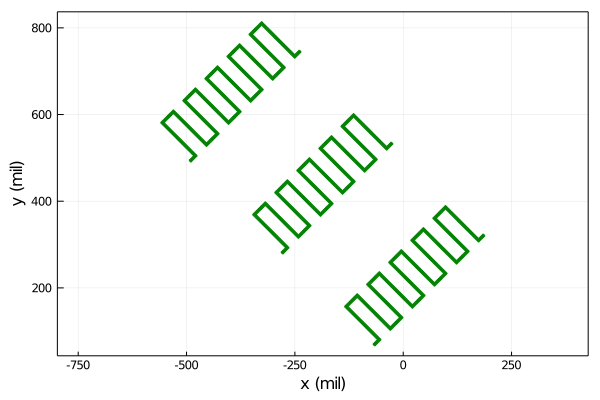
\includegraphics[scale=0.5,trim=150 50 100 20,clip=true]{meanderlines.png} \qquad \quad
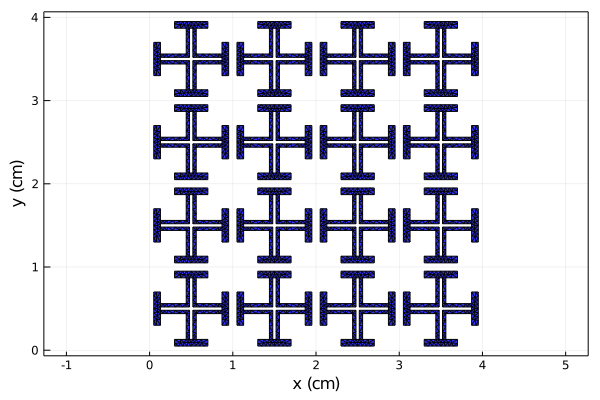
\includegraphics[scale=0.5,trim=150 50 100 20,clip=true]{jcrossarray.png}
}

\vspace{1.5in}

This document is licensed under the Creative Commons Attribution 4.0 International License.
To view a copy of this license, visit \url{http://creativecommons.org/licenses/by/4.0/}
or send a letter to Creative Commons, PO Box 1866, Mountain View, CA 94042, USA. 


% \begin{abstract}
% \lipsum[1-2]
% \end{abstract}

\clearpage

\tableofcontents*
\clearpage


\chapter{Introduction}
These notes constitute the theory documentation for the \pssfss\
program.  \pssfss\ is a \href{https://julialang.org/}{Julia} \cite{bezanson2017julia} program for the analysis
of polarization and frequency selective surfaces (PSSs and FSSs). The
structure under consideration may contain any number of 
stratified dielectric \emph{layers}, possibly including one or more
zero-thickness conducting\footnote{imperfect conductors 
are also allowed} \emph{sheets} located at the dielectric interface
layers.  The metalization pattern on the sheets is 
assumed to exhibit a two-dimensional periodicity, which may vary from
sheet to sheet.  The structure is illuminated by 
a monochromatic plane wave incident at an arbitrary angle, and the
goal of this analysis is to efficiently compute the complex scattering
matrix whose entries are reflection and transmission coefficients for
the scattered plane waves.  Various performance parameters can be obtained
from the scattering matrix, such as reflection and transmission
coefficients, axial ratio, polarization purity, delta insertion phase
delay, etc.  

To calculate the fields scattered from the metallic sheets, we will
use one of two approaches, depending on the sheet geometry:
\begin{enumerate}
\item If a sheet's unit cell of periodicity is mostly absent of
  metalization (``wire'', ``strip'', or ``capacitive'' type FSSs are
  typical examples of this), 
  it is more efficient to replace the metalization
  with unknown induced electric surface current, which will be
  solved for in the course of the analysis.
\item Alternatively, if the unit cell is mostly metalized (as in a
  ``slot'' or ``inductive'' type of FSS), then it is
  more efficient to solve for the tangential electric field in the
  non-metalized (``void'') area.  In practice this is done by filling
  in the void regions 
  with metalization and impressing upon these regions induced
  (fictitious) magnetic surface current.  Note that this technique can
  only be used when the metalization is assumed to be perfectly
  conducting.  Lossy conducting metalization requires the use of
  electric surface currents.
\end{enumerate}

The unknown electric or magnetic surface currents in the unit cell are
approximately determined by solving a mixed-potential integral
equation using
the method of moments in conjunction with the so-called ``RWG''
triangle subdomain basis functions \cite{rawg:82}. 

Each sheet in the structure is characterized by its generalized
scattering matrix (GSM).  ``Generalized'' refers to the fact that both
propagating and evanescent modes are treated.  The GSMs of the sheets
and dielectric layers are cascaded to obtain the GSM of the entire
structure. If the sheets do not all share the same periodic lattice,
then the sheet interactions are approximated by accounting only for
the dominant, propagating TE and TM modes during the cascading
process.  Also, if a sheet is surrounded by very thin dielectric
layers, then it would require a very large number of evanescent modes
to correctly model the effects of these layers.  So in this case, the
composite GSM of the sheet together with its surrounding thin layers
is directly computed, by
using a Green's function for multiply stratified dielectric layers.

This document is organized as follows:
\begin{description}[align=left]
  \item[Chapter~\ref{chap:fund}] documents the basic assumptions and
  fundamental equations for the fields and potentials needed in the
  rest of the analysis.
  \item[Chapter~\ref{chap:periodicity}] describes the type of
  periodic structures treated in this analysis, defines the direct and
  reciprocal lattices, and derives the form of Floquet modes used in
  subsequent chapters.
  \item[Chapter~\ref{chap:gsm}] defines the generalized 
  scattering matrix (GSM), and derives formulas for the GSMs of
  canonical structures needed later in the analysis.
  \item[Chapter~\ref{chap:mpgf}] derives an efficient, wide-band
  formula for the potential Green's functions for abutted half-spaces
  under quasi-periodic (Floquet) boundary conditions, as needed for
  FSS and PSS sheets that are surrounded by reasonably thick adjacent
  dielectric layers.
  \item[Chapter~\ref{chap:gfstratified}] extends this formulation to
  multiply stratified media on each side of the sheet, as is needed for
  a sheet immediately adjacent to one or more very thin dielectric
  layers.
  \item[Chapter~\ref{chap:incgsm}] discusses how to calculate the
  incident fields and extract scattering matrix entries from computed 
  currents.
  \item[Chapter~\ref{chap:mom}] provides the details of the method of
    moments (MoM) solution of the mixed potential integral equations for  
    the electric or magnetic currents flowing on the FSS/PSS sheets.
    Care is taken to exploit the wide-band nature of the Green's
    functions to minimize matrix fill time for multi-frequency
    analysis.
\end{description}


\mainmatter

\chapter{Fundamentals}
\label{chap:fund}
This chapter documents the definitions for fields, potentials, and 
Fourier transforms that are employed in remainder of this document.


We restrict consideration to time-harmonic sources in simple, linear media,
assuming and suppressing
a time dependence of $e^{j\omega t}$.  RMS phasers are used throughout, employing
rationalized MKS units. Thus,
if $V$ is a (complex) phaser voltage, then the corresponding function of time
is $v(t) = \sqrt{2} \Real{V e^{j\omega t}}$.

A right-handed Cartesian  coordinate system is adopted, with $x$, $y$, and 
$z$ axes, and unit vectors $\x$, $\y$, and $\z$.  A point $P = (x,y,z)$ is 
typically identified by the vector $\r = x\x + y\y + z\z$ which measures 
the displacement of $P$ from the origin.

The medium under consideration is characterized by its scalar, complex permittivity
$\epsilon$ [F/m] and its scalar, complex permeability $\mu$ [H/m], 
both of which may be functions 
of position, $\epsilon = \epsilon(\r)$, $\mu = \mu(\r)$. Although these parameters are
both positive for lossless media, in the presence of electric and/or magnetic
losses the imaginary part of $\epsilon$ and/or $\mu$, respectively, is negative.
Thus, $\epsilon$ and $\mu$ both lie in the fourth quadrant (or positive real
axis) of the complex plane.

For convenience we define the medium's intrinsic wavenumber
\begin{equation}
  k = \omega \sqrt{\mu\epsilon} \qquad \text{(fourth quadrant)}
\end{equation}
and intrinsic impedance
\begin{equation}
  \eta = \sqrt{\mu/\epsilon} \qquad \left(\abs{\arg\eta} < \frac{\pi}{4} \right),
\end{equation}
which, of course, vary with position if $\epsilon$ or $\mu$ do.

%%%%%%%%%%%%%%%%%%%%%%%%%%%%%%%%%%%%%%%%%%%%%%%%%%%%%%%%%%%%%%%%%%%%%%%%%%%%%%%%%%%%%%%
\section{Maxwell's Equations and Potentials for Electric Sources}
Under the assumptions listed above, and postulating the existence of only
electric sources, Maxwell's curl equations 
(Ampere's Law and Faraday's Law) take the form
\begin{subequations}
  \begin{align}
    \curl \H &= j\omega\epsilon \E + \J \label{eq:AmpereE} \\
    \curl \E &= -j\omega\mu \H  \label{eq:FaradayE}
  \end{align}
\end{subequations}
where $\E$ is the electric field vector [V/m], $\H$ is the magnetic field
vector [A/m], and $\J$ is the electric current density [A/m$^2$].
When combined with the equation of continuity
\begin{equation}
  \divergence \J + j\omega\qe = 0
\end{equation}
we obtain the divergence relations
\begin{subequations}
  \begin{align}
    \divergence \epsilon\E &= \qe  \label{eq:divE}\\
    \divergence \mu\H       &= 0,
  \end{align}
\end{subequations}
where $\qe$ is the electric charge density,
with units of [C/m$^3$].
The fact that $\mu\H$ is divergenceless leads to 
the introduction of the magnetic vector potential $\A$
having units of [Vs/m]:
\begin{equation}
  \boxed{
  \mu\H = \curl \A.  
  } \label{eq:curlA}
\end{equation}
Substituting \eqref{eq:curlA} into \eqref{eq:FaradayE} we find that
$-\E - j\omega\A$ is curl-free, and so can be written as the gradient
of the so-called electric scalar potential $\Phi$ [V]:
\begin{equation}
  \label{eq:PhiE}
  \boxed{
  \E = -j\omega\A-\gradient\Phi.
  }
\end{equation}
To derive the differential equations for $\A$ and $\Phi$ we
begin with the identity
\begin{equation}
  \curl \curl \A = \curl \mu\H = \mu \curl \H + \gradient\mu \cross \H
\end{equation}
and use Equations \eqref{eq:AmpereE} and \eqref{eq:curlA} to eliminate
$\H$:
\begin{equation}
  \gradient\divergence\A - \vlaplace\A =
  j\omega\epsilon\mu\E + \mu\J + \gradient\mu \cross 
  \left(
    \frac{1}{\mu} \curl\A
  \right).
\end{equation}
Note that we also employed the identity $\curl\curl\A = 
  \gradient\divergence\A - \vlaplace\A$.
Now eliminating $\E$ using \eqref{eq:PhiE} we obtain
\begin{equation}
  \vlaplace\A + k^2 \A + \gradient\mu \cross
  \left(
    \frac{1}{\mu} \curl\A
  \right)
  - \gradient 
  \left[
    \divergence\A + j\omega\mu\epsilon\Phi
  \right]
  = -\mu\J.
\end{equation}
Since the divergence of the magnetic vector potential is as yet unspecified,
we may apply the Lorentz gauge, $\divergence\A = -j\omega\epsilon\mu\Phi$,
and set the quantity in square brackets above to zero:
\begin{equation}
  \boxed{%
  \vlaplace\A + k^2 \A + \frac{\gradient\mu}{\mu} \cross \curl\A
  = -\mu\J.  \label{eq:WaveAinhom}
  }
\end{equation}
Equation~\eqref{eq:WaveAinhom} is the fundamental wave equation for 
the magnetic vector potential under the Lorentz gauge in an inhomogeneous
medium.  

An equation for $\Phi$ is now obtained by employing the
identity $\divergence \epsilon\E = \E\bdot\gradient \epsilon
+ \epsilon \divergence\E$ in \eqref{eq:divE} and then
eliminating $\E$ using \eqref{eq:PhiE}:
\begin{align}
  \qe
  &= \E \bdot \gradient \epsilon + \epsilon \divergence\E \notag \\
  &= -(j\omega\A + \gradient\Phi) \bdot \gradient\epsilon
  - \epsilon \divergence (j\omega\A + \gradient\Phi).
\end{align}
After invoking the Lorentz gauge this can be written as
\begin{equation}
  \boxed{%
  \laplace\Phi + k^2\Phi + \frac{\gradient\Phi \bdot \gradient\epsilon}{\epsilon}
  = 
  -\frac{\qe}{\epsilon} - \frac{j\omega\A \bdot \gradient\epsilon}{\epsilon}.
  } \label{eq:WavePhiinhom}
\end{equation}
Equation~\eqref{eq:WavePhiinhom} is the wave equation for 
the electric scalar potential under the Lorentz gauge in an inhomogeneous
medium.  

\subsection{Piecewise Homogeneous Medium}
Suppose that the spatial domain $U$ of the boundary value problem
for which Maxwell's Equations are to be
solved consists of a disjoint union of a finite number $N$ of
homogeneous regions $U_i$, as in the case of a stratified medium:
\begin{equation}
  U = \union_{i=1}^{N} U_i,
\end{equation}
and suppose that the permittivity and permeability of the $i$th region
are the constants $\epsilon_i$ and $\mu_i$, respectively, with corresponding
wavenumber $k_i$.  Then, for
points within the $i$th medium, the terms involving the gradient of
the permittivity and permeability are zero, and the 
potentials within the $i$th region are solutions to 
\begin{subequations}
  \begin{gather}
    \vlaplace\A^{(i)} + k_i^2 \A^{(i)}  = -\mu_i\J, \\
    \laplace\Phi^{(i)} + k_i^2 \Phi^{(i)}  = -\qe/\epsilon_i.
  \end{gather}
\end{subequations}
If the $i$th region contains no sources, then the potentials
in that region are solutions to the Helmholtz equation:
\begin{subequations}
  \begin{gather}
    \vlaplace\A^{(i)} + k_i^2 \A^{(i)}  = \0, \\
    \laplace\Phi^{(i)} + k_i^2 \Phi^{(i)}  = 0.
  \end{gather}
\end{subequations}

%%%%%%%%%%%%%%%%%%%%%%%%%%%%%%%%%%%%%%%%%%%%%%%%%%%%%%%%%%%%%%%%%%%%%%%%%%%%%%%%%%%%%%%
\section{Maxwell's Equations for Magnetic Sources}
Under the assumptions listed in the introduction, and postulating the existence of only
magnetic sources, Maxwell's curl equations 
(Ampere's Law and Faraday's Law) take the form
\begin{subequations}
  \begin{align}
    \curl \H &= j\omega\epsilon \E \label{eq:AmpereM} \\
    \curl \E &= -j\omega\mu \H - \M \label{eq:FaradayM}
  \end{align}
\end{subequations}
where $\E$ is the electric field vector [V/m], $\H$ is the magnetic field
vector [A/m], and $\M$ is the magnetic current density [V/m$^2$].
When combined with the equation of continuity
\begin{equation}
  \divergence \M + j\omega\qm = 0
\end{equation}
we obtain the divergence relations
\begin{subequations}
  \begin{align}
    \divergence \epsilon\E &= 0  \label{eq:divEm}\\
    \divergence \mu\H &= \qm,    \label{eq:divHm}
  \end{align}
\end{subequations}
where $\qm$ is the magnetic charge density,
with units of [Wb/m$^3$].
The fact that $\epsilon\E$ is divergenceless leads to 
the introduction of the electric vector potential $\F$
having units of [As/m]:
\begin{equation}
  \boxed{
  \epsilon\E = \curl \F.  
  } \label{eq:curlF}
\end{equation}
Substituting \eqref{eq:curlF} into \eqref{eq:AmpereM} we find that
$j\omega\F - \H$ is curl-free, and so can be written as the gradient
of the so-called magnetic scalar potential $\Psi$ [A]:
\begin{equation}
  \label{eq:PsiM}
  \boxed{
  \H =  j\omega\F - \gradient\Psi.
  }
\end{equation}
To derive the differential equations for $\F$ and $\Psi$ we
begin with the identity
\begin{equation}
  \curl \curl \F = \curl \epsilon\E = \epsilon \curl \E + \gradient\epsilon \cross \E
\end{equation}
and use Equations \eqref{eq:FaradayM} and \eqref{eq:curlF} to eliminate
$\E$:
\begin{equation}
  \gradient\divergence\F - \vlaplace\F =
  -j\omega\epsilon\mu\H - \epsilon\M + \gradient\epsilon \cross 
  \left(
    \frac{1}{\epsilon} \curl\F
  \right).
\end{equation}
Note that we also employed the identity $\curl\curl\F = 
  \gradient\divergence\F - \vlaplace\F$.
Now eliminating $\H$ using \eqref{eq:PsiM} we obtain
\begin{equation}
  \vlaplace\F + k^2 \F + \gradient\epsilon \cross
  \left(
    \frac{1}{\epsilon} \curl\F
  \right)
  - \gradient 
  \left[
    \divergence\F - j\omega\mu\epsilon\Psi
  \right]
  = \epsilon\M.
\end{equation}
Since the divergence of the electric vector potential is as yet unspecified,
we may apply the Lorentz gauge, $\divergence\F = j\omega\epsilon\mu\Psi$,
and set the quantity in square brackets above to zero:
\begin{equation}
  \boxed{%
  \vlaplace\F + k^2 \F + \frac{\gradient\epsilon}{\epsilon} \cross
  \curl\F
  = \epsilon\M.
  \label{eq:WaveFinhom}
  }
\end{equation}
Equation~\eqref{eq:WaveFinhom} is the fundamental wave equation for 
the electric vector potential under the Lorentz gauge in an inhomogeneous
medium.  

An equation for $\Psi$ is now obtained by employing the
identity $\divergence \mu\H = \H\bdot\gradient \mu
+ \mu \divergence\H$ in \eqref{eq:divHm} and then
eliminating $\H$ using \eqref{eq:PsiM}:
\begin{align}
  \qm
  &= \H \bdot \gradient \mu + \mu \divergence\H \notag \\
  &= (j\omega\F - \gradient\Psi) \bdot \gradient\mu
  + \mu \divergence (j\omega\F - \gradient\Psi).
\end{align}
After invoking the Lorentz gauge this can be written as
\begin{equation}
  \boxed{%
  \laplace\Psi + k^2\Psi + \frac{\gradient\Psi \bdot \gradient\mu}{\mu}
  = 
  -\frac{\qm}{\mu} + \frac{j\omega\F \bdot \gradient\mu}{\mu}.
  } \label{eq:WavePsiinhom}
\end{equation}
Equation~\eqref{eq:WavePsiinhom} is the wave equation for 
the electric scalar potential under the Lorentz gauge in an inhomogeneous
medium.  

\subsection{Piecewise Homogeneous Medium}
Suppose that the spatial domain $U$ of the boundary value problem
for which Maxwell's Equations are to be
solved consists of a disjoint union of a finite number $N$ of
homogeneous regions $U_i$, as in the case of a stratified medium:
\begin{equation}
  U = \union_{i=1}^{N} U_i,
\end{equation}
and suppose that the permittivity and permeability of the $i$th region
are the constants $\epsilon_i$ and $\mu_i$, respectively, with corresponding
wavenumber $k_i$.  Then, for
points within the $i$th medium, the terms involving the gradient of
the permittivity and permeability are zero, and the 
potentials within the $i$th region are solutions to 
\begin{subequations}
  \begin{gather}
    \vlaplace\F^{(i)} + k_i^2 \F^{(i)}  = \epsilon_i\M, \\
    \laplace\Psi^{(i)} + k_i^2 \Psi^{(i)}  = -\qm/\mu_i.
  \end{gather}
\end{subequations}
If the $i$th region contains no sources, then the potentials
in that region are solutions to the Helmholtz equation:
\begin{subequations}
  \begin{gather}
    \vlaplace\F^{(i)} + k_i^2 \F^{(i)}  = \0, \\
    \laplace\Psi^{(i)} + k_i^2 \Psi^{(i)}  = 0.
  \end{gather}
\end{subequations}

\section{Duality}
We note that the cases of electric-only and magnetic-only sources are duals.
Any valid equation involving electromagnetic quantities has a dual equation
which can be obtained by applying the following rules:
\begin{enumerate}
\item Interchange $\mu$ and $\epsilon$.
\item Electric quantities are replaced by their corresponding magnetic quantity.
\item Magnetic quantities are replaced by the negative of their corresponding electric quantity.
\end{enumerate}
The mappings between original and dual quantities are given in 
Table~\ref{tab:duals}.
\begin{table}[htbp]
  \begin{center}
    \leavevmode
    \begin{tabular}{|c|} \hline
      \bfseries Original $\boldsymbol{\rightarrow}$ Dual \\ \hline \hline
      $\mu \rightarrow \epsilon$ \\ \hline
      $\epsilon \rightarrow \mu$ \\ \hline
      $k \rightarrow k$ \\ \hline
      $\eta \rightarrow 1/\eta$ \\ \hline
      $\E \rightarrow \H$ \\ \hline
      $\J \rightarrow \M$ \\ \hline
      $\F \rightarrow \A$ \\ \hline
      $\Phi \rightarrow \Psi$ \\ \hline
      $\qe \rightarrow \qm$ \\ \hline
      $\H \rightarrow -\E$ \\ \hline
      $\M \rightarrow -\J$ \\ \hline
      $\A \rightarrow -\F$ \\ \hline
      $\Psi \rightarrow -\Phi$ \\ \hline
      $\qm \rightarrow -\qe$ \\ \hline
    \end{tabular}
    \caption{Electromagnetic dual quantities.}
    \label{tab:duals}
  \end{center}
\end{table}

\section{Fourier Transform Definitions}
\subsection{One-dimensional Transform}
The Fourier transform of a function $f: \Realnum \rightarrow \Complexnum$
is $\tilde{f} = \Fourier \{f\}$, where
\begin{equation}
  \tilde{f}(k) = \int_{-\infty}^{\infty} f(x) e^{jkx} \d x,
\end{equation}
so that 
\begin{equation}
  f(x) = \frac{1}{2\pi} \int_{-\infty}^{\infty} \tilde{f}(k) e^{-jkx} \d k.
\end{equation}

The completeness statement is
\begin{equation}
  \delta(x) = \frac{1}{2\pi} \int_{-\infty}^{\infty} e^{\pm jkx} \d k
\end{equation}
and Parseval's relation is
\begin{equation}
\int_{-\infty}^{\infty} f(x) g^*(x) \, \d x =   
\frac{1}{2\pi} \int_{-\infty}^{\infty} \tilde{f}(k) \tilde{g}^*(k) \, \d k.
\end{equation}
Finally, if 
\begin{equation}
  h(x) = \int_{-\infty}^{\infty} f(x') g(x-x') \, \d x'
\end{equation}
then the convolution theorem states that
\begin{equation}
  \tilde{h}(k) = \tilde{f}(k) \tilde{g}(k).
\end{equation}


\subsection{Two-dimensional Transform}
The Fourier transform of a function $f: \Realnum \times \Realnum
\rightarrow \Complexnum$
is $\tilde{f} = \Fourier \{f\}$, where
\begin{equation}
  \tilde{f}(k_x,k_y) = 
  \int_{-\infty}^{\infty}\int_{-\infty}^{\infty} 
  f(x,y) e^{j(k_x x + k_y y)} \d x  \d y,
\end{equation}
so that 
\begin{equation}
  f(x,y) = \frac{1}{4\pi^2} 
  \int_{-\infty}^{\infty}\int_{-\infty}^{\infty}
 \tilde{f}(k_x,k_y) e^{-j(k_x x + k_y y)} \d k_x  \d k_y.
\end{equation}

The completeness statement is
\begin{equation}
  \delta(x) \delta(y) = \frac{1}{4\pi^2} 
  \int_{-\infty}^{\infty}\int_{-\infty}^{\infty}
  e^{\pm j(k_x x + k_y y)} \d k_x  \d k_y
\end{equation}
and Parseval's relation is
\begin{equation}
\int_{-\infty}^{\infty} \int_{-\infty}^{\infty}
 f(x,y) g^*(x,y) \, \d x  \d y =   
\frac{1}{4\pi^2} \int_{-\infty}^{\infty} \int_{-\infty}^{\infty} 
\tilde{f}(k_x,k_y) \tilde{g}^*(k_x,k_y) \, \d k_x  \d k_y.
\end{equation}
Finally, if 
\begin{equation}
  h(x,y) = \int_{-\infty}^{\infty}\int_{-\infty}^{\infty}
 f(x',y') g(x-x',y-y') \, \d x'  \d y'
\end{equation}
then the convolution theorem states that
\begin{equation}
  \tilde{h}(k_x,k_y) = \tilde{f}(k_x,k_y) \tilde{g}(k_x,k_y).
\end{equation}




\chapter{Periodicity, Reciprocal Lattice, Floquet Modes}
\label{chap:periodicity}

This chapter discusses the direct and reciprocal lattice vectors, and
defines the Floquet modes that can exist in the dielectric regions.

\section{The Direct Lattice}
We consider a structure with discrete translational invariance in two space
dimensions.  The periodicity is characterized by the {\em direct lattice
  vectors} $\s_1$ and $\s_2$, a pair of real vectors satisfying
\begin{equation}
  \s_1 \bdot \z = \s_2 \bdot \z = 0, \quad A \equiv \z \bdot \s_1 \cross \s_2 > 0.
\end{equation}
The structure is invariant to a translation consisting of any integer number of
shifts in the $\s_1$ or $\s_2$ directions.  Such periodicity
is exhibited by idealized models of frequency selective surfaces
(FSSs) and phased arrays, for example.
This periodicity gives rise to the concept of the {direct lattice},
the set of points $\vecrho_{mn} = \x x_{mn} + \y y_{mn}$ satisfying
\begin{equation}
  \vecrho_{mn} = m \s_1 + n \s_2, \quad \text{for $m$ and $n$ any integers.}
\end{equation}
A periodic structure and its direct lattice is shown in
Figure~\ref{fig:direct}.
\begin{figure}[htbp]
  \begin{center}
        \fbox{%
      \psset{unit=0.005in}
      \pspicture*(-1,-10)(660,410)
                                % Paint it on a white, opaque background:
      \psframe*[linecolor=white,fillcolor=white,fillstyle=solid](-1,-10)(660,410)
      \multips(-60.62,-105.0)(60.62,105.0){5}%
      {%
        \multips(-242.48,0)(121.24,0){8}%
        {%
          \pspolygon(73.68,18.0)(108.18,18)(130.77,52.5)%
          (108.18,87.0)(73.68,87.0)(51.096,52.5)%
          %
          \psline[linestyle=dashed,linewidth=0.5pt](0,0)(121.24,0)
          \psline[linestyle=dashed,linewidth=0.5pt](0,0)(60.62,105.0)
          \qdisk(0,0){1.5pt}
        }%
      }
    \rput(181.86,105){%
      \psline[linewidth=1pt]{->}(0,0)(121.24,0)
      \psline[linewidth=1pt]{->}(0,0)(60.62,105.0)
      \rput(90,-13){$\s_1$}
      \rput[l](10,90){$\s_2$}
      }
    \endpspicture
      }
    \caption{A frequency selective surface consisting of a thin metal plate
        with hexagonal perforations, and the associated direct
        lattice. The location selected for the lattice origin is arbitrary.}
    \label{fig:direct}
  \end{center}
\end{figure}

\section{Periodic Boundary Conditions and the Unit Cell}
\label{sec:pbcuc}
We now assume that an electromagnetic excitation of some type is
applied to the structure.  In the case of a FSS, the excitation takes
the form of an incident plane wave.  In the case of a phased array,
the excitation may be an incident plane wave, or perhaps a set of
incoming waveguide modes in each of the excitation ports of the
radiating elements.  Denote the spatial variation of the excitation by
the function $V(\r)$.  We insist that the function $V$ satisfy the
following quasi-periodicity condition:
\begin{equation}
  \label{eq:floquetbc}
  V(\r + m\s_1 + n\s_2) = V(\r) e^{-j(m\psi_1 + n\psi_2)}, \quad
  \text{for any integers $m$ and $n$}
\end{equation}
where $\psi_1$ and $\psi_2$ are given real numbers, which we will
refer to as the ``unit cell incremental phase shifts''.  By the
translational invariance of Maxwell's equations and given the discrete
translational invariance of the structure, it is clear that all
electromagnetic fields, charges, etc., resulting from the given
excitation must also satisfy \eqref{eq:floquetbc}, which we refer to
as the ``Floquet boundary condition.''

Since the fields throughout the structure satisfy
Equation~\eqref{eq:floquetbc}, it suffices to restrict consideration
to a single unit cell $U$, defined\footnote{The definition of a unit
  cell is not unique.  The present definition is most useful for our
  purposes.}
as the set of points $\r$
satisfying
\begin{equation}
  \label{eq:unitcell}
  U = \{\r: \; \r = \xi_1 \s_1 + \xi_2 \s_2 + \z z, \quad 0 \leq \xi_1 , \xi_2
  \leq 1\},
\end{equation}
where $\xi_1$ and $\xi_2$ are the so-called ``normalized area
coordinates,'' each constrained to the interval $[0,1]$.
We seek a set of modes that can propagate in the unit cell, subject to
an appropriate set of boundary conditions to be stated below.  Let
$E(\r)$ be some rectangular component of electric or magnetic field
evaluated at a point $\r = \x x + \y y + \z z = \xi_1 \s_1 + \xi_2
\s_2 + \z z$ within the unit cell.  
%Let $f(\xi_1,\xi_2) = 
%E(\xi_1\s_1+\xi_2\s_2+\z z) =E(\r)$.
Then the quasi-periodic boundary condition can be expressed as
\begin{subequations}
  \label{eq:cellfloquetbc}
  \begin{align}
    E(\s_1 + \xi_2 \s_2 + \z z) &= E(\xi_2 \s_2 + \z z) e^{-j\psi_1} \\
    E(\xi_1 \s_1 + \s_2 + \z z) &= E(\xi_1 \s_1 + \z z) e^{-j\psi_2} 
  \end{align}
\end{subequations}
  which must hold for all $z$ and for all $\xi_1$ and $\xi_2$ in the
  interval $[0,1]$.  
\subsection{Mode Potentials}

Following the formalism of Section~5.1 of \cite{coll:91}, for both TE
and TM modes we seek mode potentials $\Psi(\vecrho) = \Psi(x,y)$ that satisfy the
two-dimensional Helmholtz equation
\begin{equation}
  \label{eq:laplace2d}
  \laplace_t \Psi + k_c^2 \Psi = 0
\end{equation}
within the unit cell in addition to the boundary 
conditions \eqref{eq:cellfloquetbc}.
To simplify the following derivation, let $f(\xi_1,\xi_2) =
\Psi(\xi_1\s_1 + \xi_2\s_2) = \Psi(x,y)$.
Then the boundary condition \eqref{eq:cellfloquetbc} satisfied by $\Psi$
can be expressed more simply in terms of $f$ as
\begin{subequations}
  \label{eq:cellfloquetbcf}
  \begin{align}
    f(1, \xi_2) &= f(0,\xi_2) e^{-j\psi_1} \\
    f(\xi_1, 1) &= f(\xi_1, 0) e^{-j\psi_2} 
  \end{align}
\end{subequations}
Note that $f$ is periodic in $\xi_1$ and $\xi_2$ with unit period 
except for the
progressive phase shifts $\psi_1$ and $\psi_2$.  This motivates us to
consider the function $f(\xi_1,\xi_2) e^{j(\xi_1\psi_1 +
  \xi_2\psi_2)}$ which is indeed periodic and can therefore be
expanded in a double Fourier series:
\begin{equation*}
  f(\xi_1,\xi_2) e^{j(\xi_1\psi_1 + \xi_2\psi_2)} = 
  \sum_{m=-\infty}^{\infty} \sum_{n=-\infty}^{\infty} \!\!\!
  f_{mn} \, e^{-j(m2\pi\xi_1 + n2\pi\xi_2)}
\end{equation*}
or equivalently
\begin{equation}
  \label{eq:fourier}
  f(\xi_1,\xi_2) =
  \sum_{m=-\infty}^{\infty} \sum_{n=-\infty}^{\infty} \!\!\!
  f_{mn} \, e^{-j[\xi_1(\psi_1+m2\pi) + \xi_2(\psi_2+n2\pi)]}.
\end{equation}
We wish to write Equation~\eqref{eq:fourier} explicitly in terms of
$\vecrho = \x x + \y y$.  Recalling that $\vecrho = \xi_1\s_1 +
\xi_2\s_2$ and writing the relation in matrix form yields
\begin{equation}
  \colvec{x\\y} = 
  \begin{bmatrix}
    s_{1x} & s_{2x} \\
    s_{1y} & s_{2y} 
  \end{bmatrix}
    \colvec{\xi_1 \\ \xi_2}.
\end{equation}
Inverting, we obtain
\begin{align}
\colvec{\xi_1 \\ \xi_2} &=
  \frac{1}{A}
  \begin{bmatrix}
    s_{2y} & -s_{2x} \\
    -s_{1y} & s_{1x} 
  \end{bmatrix}
      \colvec{x\\y} \nonumber \\
      &=
      \frac{1}{A}
      \colvec{s_{2y}x -s_{2x}y \\
        -s_{1y}x + s_{1x}y}  \nonumber \\
      &=
      \frac{1}{A}
      \colvec{\s_2 \cross \z \bdot \vecrho \\
        \z \cross \s_1 \bdot \vecrho}  \nonumber \\
      &=
      \frac{1}{2\pi}
      \colvec{
        \vecbeta_1 \bdot \vecrho \\
        \vecbeta_2 \bdot \vecrho
        }
\end{align}
where 
\begin{equation}
  \label{eq:betadef}
  \vecbeta_1 = \frac{2\pi}{A} \s_2\cross\z, \quad
  \vecbeta_2 = \frac{2\pi}{A} \z \cross \s_1,
\end{equation}
are the {\em reciprocal lattice vectors} \cite{dufo:67,kitt:66}
and $A = \z \bdot \s_1 \cross \s_2$ is the area of the unit cell.
Substituting \eqref{eq:betadef} into \eqref{eq:fourier}, we obtain the
desired representation of the mode potential:
\begin{equation}
    f(\xi_1,\xi_2) = \Psi(x,y) = 
  \sum_{m=-\infty}^{\infty} \sum_{n=-\infty}^{\infty}
  f_{mn} e^{-j\vecbeta_{mn} \bdot \vecrho}
\end{equation}
where 
\begin{subequations}
  \begin{align}
    \vecbeta_{mn} &= \vecbeta_{00} + m\vecbeta_1 + n\vecbeta_2, \\
    \vecbeta_{00} &= \frac{\psi_1}{2\pi}\vecbeta_1 +  \frac{\psi_2}{2\pi}\vecbeta_2. 
  \end{align}
\end{subequations}
We see that the mode potentials assume the form of a discrete set of plane waves for
both TE and TM modes.  The cutoff wavenumber $k_c$ of a plane wave
with transverse propagation vector $\vecbeta_{mn}$ is given by 
\begin{equation}
  k_c = \beta_{mn} \equiv \sqrt{\vecbeta_{mn} \bdot \vecbeta_{mn}}.
\end{equation}
For a lossless medium a finite number of modes may satisfy $k >
\beta_{mn}$; these are the propagating modes.  The remaining modes,
comprising a denumerably infinite set, are cut-off (or evanescent).
The situation is depicted in Figure~\ref{fig:reciprocal} for the
structure of Figure~\ref{fig:direct}.
\begin{figure}[tbp]
  \begin{center}
        \fbox{%
      \psset{unit=0.006in}
      \pspicture*(20,10)(660,400)
                                % Paint it on a white, opaque background:
      \psframe*[linecolor=white,fillcolor=white,fillstyle=solid](20,10)(660,400)
      \multips(-105,303.1)(105.0,-60.62){8}%
      {%
        \multips(0,-242.48)(0,121.24){8}%
        {%
          \psline[linestyle=dashed,linewidth=0.5pt](0,0)(0,121.24)
          \psline[linestyle=dashed,linewidth=0.5pt](0,0)(105.0,-60.62)
          \psline[linewidth=1pt]{->}(0,0)(35,25)
          \qdisk(0,0){1.5pt}
        }%
      }
    \rput(315,181.86){%
      \psline[linewidth=1pt]{->}(0,0)(105.0,-60.62)
      \psline[linewidth=1pt]{->}(0,0)(0,121.24)
      \rput(75,-65){$\vecbeta_1$}
      \rput(-20,95){$\vecbeta_2$}
      \pscircle[linewidth=0.75pt,linestyle=dashed](0,0){70}
      \rput*(62,25){$\vecbeta_{0,0}$}
      }
    \endpspicture
      }
    \caption[Reciprocal lattice.]{The reciprocal lattice for the
      structure of Figure~\ref{fig:direct}.  Note that this lattice is
        a scaled and rotated (by $90^\circ$) version of the direct
        lattice. 
        Modes are located at the tips of the small, offset vectors.
        Propagating modes lie within the dashed circle of radius $k$
        centered on the origin.  The offset vector $\vecbeta_{00}$
        accounts for the effects of the impressed phase shift.
        }
    \label{fig:reciprocal}
  \end{center}
\end{figure}


Following the prescription given in \cite{coll:91}, we may now write
down the explicit forms of the modal fields:

\subsection{TE modes}
\label{sec:temodes}

\subsubsection{Oblique Incidence}
We first assume that $\beta_{mn} \neq 0$, in which case 
the modal fields are
\begin{subequations}
  \label{eq:TEmodes}
  \begin{align}
    \Psi_{mn}\TE(\vecrho) &= \frac{c_{mn}\TE}{k\eta\beta_{mn}}
    e^{-j\vecbeta_{mn} \bdot \vecrho} \\
    \gamma_{mn} &= \sqrt{\beta_{mn}^2 - k^2} \qquad \text{(1st quadrant)} \\
    Z_{mn}\TE &= \frac{1}{Y_{mn}\TE} = \frac{jk\eta}{\gamma_{mn}} \\
    (\x\x+\y\y) \bdot \H_{mn}\TE(\r) &= \pm \gamma_{mn} e^{\pm\gamma_{mn}z}
    \,\gradient_t \Psi_{mn}\TE \nonumber \label{eq:htransTE} \\
    &= \mp j \gamma_{mn} \Psi_{mn}\TE e^{\pm\gamma_{mn}z}  \vecbeta_{mn}
    \nonumber \\
    &= \pm c_{mn}\TE Y_{mn}\TE e^{-j\vecbeta_{mn}\bdot\vecrho \pm
      \gamma_{mn} z} \betahat_{mn}
    \\
    \z \bdot \H_{mn}\TE(\r) &= \beta_{mn}^2 \Psi_{mn}\TE
    e^{\pm\gamma_{mn} z} \nonumber  \\
    &= c_{mn}\TE \frac{\beta_{mn}}{k\eta} e^{-j\vecbeta_{mn}\bdot\vecrho \pm
      \gamma_{mn} z} \\
    \E_{mn}\TE(\r) &= \pm Z_{mn}\TE \z \cross \H_{mn}(\r) \nonumber \\
     &= c_{mn}\TE  e^{-j\vecbeta_{mn}\bdot\vecrho \pm \gamma_{mn} z}
     \z\cross\betahat_{mn} \label{eq:etransTE}
  \end{align}
\end{subequations}
where we have used  $  \betahat_{mn} = \vecbeta_{mn} / \beta_{mn}$.




\subsubsection{Normal Incidence}
In the case where $\beta_{mn} = 0$, we use the following convention:
\begin{equation}
  \betahat_{mn} = \x, \label{eq:betahatnormal}
\end{equation}
so that the final formulas in \eqref{eq:TEmodes} remain valid.

\subsection{TM modes}
\label{sec:tmmodes}

\subsubsection{Oblique Incidence}
We first assume that $\beta_{mn} \neq 0$, in which case 
\begin{subequations}
  \label{eq:TMmodes}
  \begin{align}
    \Psi_{mn}\TM(\vecrho) &= \frac{\pm j c_{mn}\TM}{\gamma_{mn}\beta_{mn}}
    e^{-j\vecbeta_{mn} \bdot \vecrho} \\
    \gamma_{mn} &= \sqrt{\beta_{mn}^2 - k^2} \qquad \text{(1st quadrant)} \\
    Y_{mn}\TM &= \frac{1}{Z_{mn}\TM} = \frac{jk}{\eta\gamma_{mn}} \\
    (\x\x+\y\y) \bdot \E_{mn}\TM(\r) &= \pm \gamma_{mn} e^{\pm\gamma_{mn}z}
    \,\gradient_t \Psi_{mn}\TM \nonumber \\
    &= 
    \mp j \gamma_{mn} \Psi_{mn}\TM e^{\pm\gamma_{mn}z}  \vecbeta_{mn}
    \nonumber \\
    &= c_{mn}\TM e^{-j\vecbeta_{mn}\bdot\vecrho \pm \gamma_{mn} z}
    \betahat_{mn} \\
    %
    \z \bdot \E_{mn}\TM(\r) &= 
    \beta_{mn}^2 \Psi_{mn}\TM e^{\pm\gamma_{mn} z} \nonumber \\
    &= \pm j c_{mn}\TM \frac{\beta_{mn}}{\gamma_{mn}} 
    e^{-j\vecbeta_{mn}\bdot\vecrho \pm \gamma_{mn} z} \\
    %
    \H_{mn}\TM(\r) &= \mp Y_{mn}\TM \z \cross \E_{mn}\TM(\r) \nonumber \\
     &= \mp c_{mn}\TM Y_{mn}\TM
     e^{-j\vecbeta_{mn}\bdot\vecrho \pm \gamma_{mn} z}
     \z\cross\betahat_{mn} 
  \end{align}
\end{subequations}

\subsubsection{Normal Incidence}
In the case where $\beta_{mn} = 0$, we again employ the convention
\eqref{eq:betahatnormal}, so that the final formulas in
\eqref{eq:TMmodes}
remain valid.

\subsection{Mode Normalization}
So far we have not specified values for 
the set of mode normalization constants $\{c_{mn}\TE\}$ and
$\{c_{mn}\TM\}$.  These can be specified in any convenient manner.  We
will choose a normalization that allows us to easily interpret the
incident and reflected traveling wave variables in terms of power
transported by the modes.  Consider a source-free slab of the unit cell bounded by
$z = \text{constant}$ planes, filled with homogeneous dielectric
material.  Taking account of the results of Sections~\ref{sec:temodes}
and~\ref{sec:tmmodes}, we see that the transverse components of the
most general electromagnetic field that can exist in
this region can be written as
\begin{subequations}
  \label{eq:modalexpansions}
  \begin{align}
    (\x\x+\y\y) \bdot \E(\r) &= 
    \mkern -15mu \sum_{(p,m,n) \in S} \mkern -15mu
    \e_{pmn}(x,y) 
    \left(
      a_{pmn} e^{-\gamma_{mn} z} + b_{pmn} e^{\gamma_{mn} z}
    \right), \\
    %
    (\x\x+\y\y) \bdot \H(\r) &= 
    \mkern -15mu \sum_{(p,m,n) \in S} \mkern -15mu
    \h_{pmn}(x,y) 
    \left(
      a_{pmn} e^{-\gamma_{mn} z} - b_{pmn} e^{\gamma_{mn} z}
    \right),
  \end{align}
\end{subequations}
where the summations are taken over the set of integer triples 
$S = \{(p,m,n) \in \{1,2\}
\cross \Integers \cross \Integers\}$, $\Integers$ is the set of
all integers, $p=1$ corresponds to TE modes, and $p=2$ corresponds to
TM modes.  The modal fields $\e_{pmn}$ and $\h_{pmn}$ are given
explicitly by
\begin{subequations}
  \label{eq:modaldefs}
  \begin{align}
    \e_{1mn} &= 
      c_{1mn}  \z \cross \betahat_{mn} e^{-j\vecbeta_{mn} \bdot \vecrho}
       \\
    %
    \e_{2mn} &= 
      c_{2mn}  \betahat_{mn} e^{-j\vecbeta_{mn} \bdot \vecrho}
      \hphantom{\z \cross \mbox{}}
      \\
    %
    \h_{pmn} &= Y_{pmn} \z \cross \e_{pmn} 
  \end{align}
\end{subequations}
where 
\begin{subequations}
  \begin{align}
    Y_{1mn} &= Y_{mn}\TE, \quad  c_{1mn} = c_{mn}\TE \\
    Y_{2mn} &= Y_{mn}\TM, \quad  c_{2mn} = c_{mn}\TM.
  \end{align}
\end{subequations}


By virtue of the orthogonality of the Floquet modes (see
Appendix~\ref{app:orthogonal}), the 
complex power P traveling down the unit cell in the $z$ direction can
be expressed as a sum of the individual complex powers transported by each mode:
\begin{align}
  P &= \iint_{U'} \E \cross \H^* \bdot \z \; \d A
  \nonumber \\
  &= \sum_{(p,m,n) \in S}
  (a_{pmn} + b_{pmn})(a_{pmn}^* - b_{pmn}^*) \iint_{U'}
  \e_{pmn} \cross \h_{pmn}^* \bdot \z \; \d A \nonumber \\
  %
  &= \sum_{(p,m,n) \in S} \mkern -16 mu
  \left[
    \abs{a_{pmn}}^2 - \abs{b_{pmn}}^2 - 2j\Imag{a_{pmn}b_{pmn}^*}
  \right]
  P_{pmn}
\end{align}
where $U'$ is the restriction of the unit cell to the plane $z=0$,
and
\begin{equation}
  P_{pmn} = \iint_{U'} \mkern -8 mu
  \e_{pmn} \cross \h_{pmn}^* \bdot \z \; \d A  
  = \abs{c_{pmn}}^2
  Y_{pmn}^* A
\label{eq:Ppmn}
\end{equation}
is the complex power associated with each unit-strength positive-going
mode.  Its value depends on the choice of mode normalization constant
$c_{pmn}$, which has not yet been specified.  Note that if $P_{pmn}$
is equal to $1$, then the time-average (real) power carried down the
guide in the $+z$ direction is just $\abs{a_{pmn}}^2 -
\abs{b_{pmn}}^2$, consistent
with the usual definition of traveling wave variables \cite{bbse:69}.
Such a normalization is not possible, since in many cases
of practical interest, $P_{\mkern -4mu pmn}$ has zero real part.
Consider the case of a lossless medium
with $\beta_{mn} > k$.  Then $\gamma_{mn}$ is pure real, so that
$Y_{pmn}$ is pure imaginary.  It follows from Equation~\eqref{eq:Ppmn}
that $P_{\mkern -4mu pmn}$ is pure imaginary, since $A$ and $\abs{c_{pmn}}$ are
both pure real.  Therefore, we content ourselves with setting the
magnitude of $P_{\mkern -4mu pmn}$ equal to $P_0 \equiv \text{one watt}$:
\begin{equation}
  P_{pmn} = \frac{Y_{pmn}^*}{\abs{Y_{pmn}}} P_0.
  \label{eq:Pset}
\end{equation}
Substituting \eqref{eq:Pset} into \eqref{eq:Ppmn} determines the value
of the mode normalization constant (up to an arbitrary phase):
\begin{equation}
  \abs{c_{pmn}} = \sqrt{\frac{P_0}{A \abs{Y_{pmn}}}}.
\end{equation}
This choice results in a unitary scattering matrix for propagating
modes in lossless media.  It will be convenient for later work to
choose the phase of $c_{pmn}$ as follows:
\begin{equation}
  c_{pmn} = \sqrt{\frac{P_0}{A Y_{pmn}}}.
  \label{eq:modenormalization}
\end{equation}
where we agree to take that square root of $Y_{pmn}$ having positive
real part.



\chapter{Generalized Scattering Matrix}
\label{chap:gsm}

\section{Introduction}
This chapter documents the form of the GSM (generalized scattering
matrix) used in the \pssfss\ program and provides
formulas for the
scattering parameters of several
canonical structures needed in the analysis of an FSS
(Frequency Selective Surface).  These
include a dielectric interface, a dielectric slab, and the
cascade interconnection of two FSS structures.


\section{Definition of the GSM}
We consider a structure with two-dimensional periodicity as described
in Chapter~\ref{chap:periodicity}.  The structure occupies the region $z_1 \leq z
\leq z_2$, as shown in Figure~\ref{fig:geom}.
%
\begin{figure}[tbp]
  \begin{center}
    \setlength{\unitlength}{0.2in}
      \small
    \begin{picture}(18,7.5)(-9,-4)
      \put(-3,-3){\line(0,1){6}}  % z1 boundary
      \put(3,-3){\line(0,1){6}}   % z2 boundary
      \put(-3,-3.5){\makebox(0,0){$z_1$}}
      \put(3,-3.5){\makebox(0,0){$z_2$}}
      \put(0,0){\makebox(0,0){%
          \begin{tabular}{@{}c@{}} 
            FSS/Radome \\
            Structure
          \end{tabular}
          }}
      \put(-3.75,2.1){\makebox(0,0){$\mat{a}^{(1)}$}}
      \put(-4,1.5){\makebox(0,0){$\longrightarrow$}}
      %
      \put(-3.75,-1.5){\makebox(0,0){$\mat{b}^{(1)}$}}
      \put(-4,-2.1){\makebox(0,0){$\longleftarrow$}}
      %
      \put(4.25,2.1){\makebox(0,0){$\mat{a}^{(2)}$}}
      \put(4,1.5){\makebox(0,0){$\longleftarrow$}}
      %
      \put(4.25,-1.5){\makebox(0,0){$\mat{b}^{(2)}$}}
      \put(4,-2.1){\makebox(0,0){$\longrightarrow$}}
      %
      \put(-7,0){\makebox(0,0){%
        \begin{tabular}{@{}c@{}}
          Region 1: \\
          $\epsilon_1$, $\mu_1$, $k_1$, $\eta_1$
        \end{tabular}}}
      %
      \put(7,0){\makebox(0,0){%
        \begin{tabular}{@{}c@{}}
          Region 2: \\
          $\epsilon_2$, $\mu_2$, $k_2$, $\eta_2$
        \end{tabular}}}
      %
    \end{picture}
    \caption[A structure to be characterized by its GSM]
    {A structure to be characterized by its GSM occupies the region
    $z_1 \leq z \leq z_2$.  It is bounded on each side by (possibly
    dissimilar) homogeneous, dielectric  half-spaces.}
    \label{fig:geom}
  \end{center}
\end{figure}
%
It is bounded by the two half-spaces denoted as Region~1 and Region~2.
Each is characterized by its electrical parameters $\mu_i$, 
$\epsilon_i$, $k_i$, and $\eta_i$, $i = 1,2$, which are the
permittivity, permeability, intrinsic wavenumber, and intrinsic
impedance, respectively.  Given the lattice vectors $\s_1$ and $\s_2$
and impressed phasings $\psi_1$ and $\psi_2$, as defined in
Chapter~\ref{chap:periodicity}, we may expand the transverse fields in
each of Regions~1 and~2 in terms of 
incident and reflected Floquet modes:
\begin{subequations}
  \begin{align}
    (\x\x+\y\y) \bdot \E\one(\r) &= 
    \sum_{q=1}^{N_1}
    \e\one_{q}(x,y) 
    \left(
      a\one_{q} e^{-\gamma\one_{q} (z-z_1)} + b\one_{q} e^{\gamma\one_{q} (z-z_1)}
    \right), \\
                                %
    (\x\x+\y\y) \bdot \H\one(\r) &= 
    \sum_{q=1}^{N_1}
    \h\one_{q}(x,y) 
    \left(
      a\one_{q} e^{-\gamma\one_{q} (z-z_1)} - b\one_{q} e^{\gamma\one_{q} (z-z_1)}
    \right), \\
    %
    (\x\x+\y\y) \bdot \E\two(\r) &= 
    \sum_{q=1}^{N_2}
    \e\two_{q}(x,y) 
    \left(
      a\two_{q} e^{\gamma\two_{q} (z-z_2)} + b\two_{q} e^{-\gamma\two_{q} (z-z_2)}
    \right), \\
                                %
    (\x\x+\y\y) \bdot \H\two(\r) &= 
    \sum_{q=1}^{N_2}
    \h\two_{q}(x,y) 
    \left(
      -a\two_{q} e^{\gamma\two_{q} (z-z_2)} + b\two_{q} e^{-\gamma\two_{q} (z-z_2)}
    \right).
  \end{align}
  \label{eq:fieldexp}
\end{subequations}

\noindent
Superscripted numbers in parentheses are used in Equations~\eqref{eq:fieldexp} 
as region designators. The sums are taken over the set of modes in each region, which
for convenience are enumerated with a single index $q$, rather than
the triple index $(p,m,n)$ as was used in Section~\ref{sec:pbcuc}.  We will
make use of both subscripting schemes,  employing whichever is most
convenient in a particular formula.  Although
the limits on the sums should be infinite in principle, the numbers of
modes in each region are truncated to a finite value ($N_1$ modes in
Region~1 and $N_2$ in Region~2) so that a numerical evaluation can be
accomplished.
In general the modes are sorted prior to enumeration so that those
with the smallest values of $\beta_{mn}$ are retained in the finite sums.


The generalized scattering matrix
 $\mat{S}$ expresses the linear relationship between the incident and
scattered Floquet modal coefficients evaluated at each terminal plane of the FSS
structure.  This relationship is written in partitioned form as
\begin{equation}
  \label{eq:gsm}
  \colvec{\mat{b}\one \\ \mat{b}\two} = 
  \begin{bmatrix}
    \mat{S}^{11} & \mat{S}^{12} \\
    \mat{S}^{21} & \mat{S}^{22} 
  \end{bmatrix}
  \colvec{\mat{a}\one \\ \mat{a}\two}
\end{equation}
where
\begin{equation}
    \mat{a}\one = 
    \colvec{a\one_1\\ a\one_2\\ a\one_3\\ \vdots \\ a\one_{N_1}},
    \quad
    \mat{b}\one = 
    \colvec{b\one_1 \\ b\one_2 \\ b\one_3 \\ \vdots \\ b\one_{N_1}},
    \quad
    \mat{a}\two = 
    \colvec{a\two_1 \\ a\two_2 \\ a\two_3 \\ \vdots \\ a\two_{N_2}},
    \quad
    \mat{b}\two = 
    \colvec{b\two_1 \\ b\two_2 \\ b\two_3 \\ \vdots \\ b\two_{N_2}},
\end{equation}
and $\mat{S}^{11} \in \Complexnum^{N_1\times N_1}$,
$\mat{S}^{12} \in \Complexnum^{N_1\times N_2}$,
$\mat{S}^{21} \in \Complexnum^{N_2\times N_1}$,
$\mat{S}^{22} \in \Complexnum^{N_2\times N_2}$.
We see that the entries of the $\mat{S}^{11}$ and $\mat{S}^{22}$
matrices are
reflection coefficients while those of $\mat{S}^{12}$ and 
$\mat{S}^{21}$ are transmission coefficients.

\section{GSM of a Dielectric Interface}
Consider the case where $z_1 = z_2 = 0$ and there is no FSS present at
the junction plane.  The resulting structure is then just the
interface between two homogeneous half-spaces.

\subsection{Wave Incident from Region~1}
\label{sec:1inc}
\subsubsection{TE Mode Incident}
\label{sec:1incTE}
The transverse components of the incident field are
\begin{subequations}
  \begin{align}
    (\x\x + \y\y) \bdot \E\inc &= c\one_{1mn}
    e^{-j\vecbeta_{mn}\bdot\vecrho - \gamma\one_{mn} z} 
    \z\cross\betahat_{mn} \\
    (\x\x + \y\y) \bdot \H\inc &= -c\one_{1mn} Y\one_{1mn}
    e^{-j\vecbeta_{mn}\bdot\vecrho - \gamma\one_{mn} z} 
    \betahat_{mn}
  \end{align}
\end{subequations}
The transverse components of the reflected field are
\begin{subequations}
  \begin{align}
    (\x\x + \y\y) \bdot \E\refl &= R\one_{1mn} c\one_{1mn}
    e^{-j\vecbeta_{mn}\bdot\vecrho + \gamma\one_{mn} z} 
    \z\cross\betahat_{mn} \\
    (\x\x + \y\y) \bdot \H\refl &= R\one_{1mn} c\one_{1mn} Y\one_{1mn}
    e^{-j\vecbeta_{mn}\bdot\vecrho + \gamma\one_{mn} z} 
    \betahat_{mn}
  \end{align}
\end{subequations}
The transverse components of the transmitted field are
\begin{subequations}
  \begin{align}
    (\x\x + \y\y) \bdot \E\trans &= T\two_{1mn} c\two_{1mn}
    e^{-j\vecbeta_{mn}\bdot\vecrho - \gamma\two_{mn} z} 
    \z\cross\betahat_{mn} \\
    (\x\x + \y\y) \bdot \H\trans &= -T\two_{1mn} c\two_{1mn} Y\two_{1mn}
    e^{-j\vecbeta_{mn}\bdot\vecrho - \gamma\two_{mn} z} 
    \betahat_{mn}
  \end{align}
\end{subequations}
The unknown reflection and transmission coefficients $R\one_{1mn}$ and
$T\two_{1mn}$ are determined by equating the total transverse electric
and magnetic fields at each side of the interface:
\begin{subequations}
  \begin{align}
    (\x\x+\y\y) \bdot \left[\E\inc(0,0,0) + \E\refl(0,0,0)\right] &= 
    (\x\x+\y\y) \bdot \E\trans(0,0,0), \\
    (\x\x+\y\y) \bdot \left[\H\inc(0,0,0) + \H\refl(0,0,0)\right] &= 
    (\x\x+\y\y) \bdot \H\trans(0,0,0).
  \end{align}
\end{subequations}
This procedure results in the following system of equations for the transmission
and reflection coefficient:
\begin{subequations}
  \label{eq:RTsystem1}
  \begin{align}
    1 + R\one_{1mn} &= \frac{c\two_{1mn}}{c\one_{1mn}} T\two_{1mn} = 
    \frac{\sqrt{Y\one_{1mn}}}{\sqrt{Y\two_{1mn}}} T\two_{1mn} 
    \label{eq:1plusR}\\
    1 - R\one_{1mn} &= \frac{c\two_{1mn} Y\two_{1mn}}{c\one_{1mn} Y\one_{1mn}}
    T\two_{1mn} = 
    \frac{\sqrt{Y\two_{1mn}}}{\sqrt{Y\one_{1mn}}} T\two_{1mn} \label{eq:1minusR}
  \end{align}
\end{subequations}
where we have made use of Equation~\eqref{eq:modenormalization}.
One can easily solve for $R\one_{1mn}$ by dividing the equations and
recalling that 
\begin{equation}
  y = \frac{1-x}{1+x}  \iff x = \frac{1-y}{1+y}.
\end{equation}
The result is 
\begin{align}
  R\one_{1mn} &= 
  \frac{Y\one_{1mn} - Y\two_{1mn}}{Y\one_{1mn} + Y\two_{1mn}} 
  = \frac{Z\two_{1mn} - Z\one_{1mn}}{Z\two_{1mn} + Z\one_{1mn}}, \\
   T\two_{1mn} &= 
   \frac{2\sqrt{Y\one_{1mn}}\sqrt{Y\two_{1mn}}}{Y\one_{1mn}+Y\two_{1mn}}
  = \frac{2\sqrt{Z\one_{1mn}}\sqrt{Z\two_{1mn}}}{Z\one_{1mn}+Z\two_{1mn}}.
\end{align}


\subsubsection{TM Mode Incident}
The transverse components of the incident field are
\begin{subequations}
  \begin{align}
    (\x\x + \y\y) \bdot \E\inc &= c\one_{2mn}
    e^{-j\vecbeta_{mn}\bdot\vecrho - \gamma\one_{mn} z} 
    \betahat_{mn} \\
    (\x\x + \y\y) \bdot \H\inc &= c\one_{2mn} Y\one_{2mn}
    e^{-j\vecbeta_{mn}\bdot\vecrho - \gamma\one_{mn} z} 
    \z\cross\betahat_{mn}
  \end{align}
\end{subequations}
The transverse components of the reflected field are
\begin{subequations}
  \begin{align}
    (\x\x + \y\y) \bdot \E\refl &= R\one_{2mn} c\one_{2mn}
    e^{-j\vecbeta_{mn}\bdot\vecrho + \gamma\one_{mn} z} 
    \betahat_{mn} \\
    (\x\x + \y\y) \bdot \H\refl &= -R\one_{2mn} c\one_{2mn} Y\one_{2mn}
    e^{-j\vecbeta_{mn}\bdot\vecrho + \gamma\one_{mn} z} 
    \z\cross\betahat_{mn}
  \end{align}
\end{subequations}
The transverse components of the transmitted field are
\begin{subequations}
  \begin{align}
    (\x\x + \y\y) \bdot \E\trans &= T\two_{2mn} c\two_{2mn}
    e^{-j\vecbeta_{mn}\bdot\vecrho - \gamma\two_{mn} z} 
    \betahat_{mn} \\
    (\x\x + \y\y) \bdot \H\trans &= -T\two_{2mn} c\two_{2mn} Y\two_{2mn}
    e^{-j\vecbeta_{mn}\bdot\vecrho - \gamma\two_{mn} z} 
    \z\cross\betahat_{mn}
  \end{align}
\end{subequations}

When the total transverse fields are equated at the plane $z=0$, we
again arrive at the set of equations \eqref{eq:RTsystem1}
for the unknowns $R\one_{2mn}$ and $T\two_{2mn}$.  Therefore, the TM
reflection and transmission coefficients for a wave incident from
Region~1 are identical to the TE coefficients:
\begin{align}
  R\one_{2mn} &= 
  \frac{Y\one_{2mn} - Y\two_{2mn}}{Y\one_{2mn} + Y\two_{2mn}} 
  = \frac{Z\two_{2mn} - Z\one_{2mn}}{Z\two_{2mn} + Z\one_{2mn}}, \\
   T\two_{2mn} &= 
   \frac{2\sqrt{Y\one_{2mn}}\sqrt{Y\two_{2mn}}}{Y\one_{2mn}+Y\two_{2mn}}
  = \frac{2\sqrt{Z\one_{2mn}}\sqrt{Z\two_{2mn}}}{Z\one_{2mn}+Z\two_{2mn}}.
\end{align}

\subsection{Wave Incident from Region~2}
\label{sec:2inc}
\subsubsection{TE Mode Incident}
The transverse components of the incident field are
\begin{subequations}
  \begin{align}
    (\x\x + \y\y) \bdot \E\inc &= c\two_{1mn}
    e^{-j\vecbeta_{mn}\bdot\vecrho + \gamma\two_{mn} z} 
    \z\cross\betahat_{mn} \\
    (\x\x + \y\y) \bdot \H\inc &= c\two_{1mn} Y\two_{1mn}
    e^{-j\vecbeta_{mn}\bdot\vecrho + \gamma\two_{mn} z} 
    \betahat_{mn}
  \end{align}
\end{subequations}
The transverse components of the reflected field are
\begin{subequations}
  \begin{align}
    (\x\x + \y\y) \bdot \E\refl &= R\two_{1mn} c\two_{1mn}
    e^{-j\vecbeta_{mn}\bdot\vecrho - \gamma\two_{mn} z} 
    \z\cross\betahat_{mn} \\
    (\x\x + \y\y) \bdot \H\refl &= -R\two_{1mn} c\two_{1mn} Y\two_{1mn}
    e^{-j\vecbeta_{mn}\bdot\vecrho - \gamma\two_{mn} z} 
    \betahat_{mn}
  \end{align}
\end{subequations}
The transverse components of the transmitted field are
\begin{subequations}
  \begin{align}
    (\x\x + \y\y) \bdot \E\trans &= T\one_{1mn} c\one_{1mn}
    e^{-j\vecbeta_{mn}\bdot\vecrho + \gamma\one_{mn} z} 
    \z\cross\betahat_{mn} \\
    (\x\x + \y\y) \bdot \H\trans &= T\one_{1mn} c\one_{1mn} Y\one_{1mn}
    e^{-j\vecbeta_{mn}\bdot\vecrho + \gamma\one_{mn} z} 
    \betahat_{mn}
  \end{align}
\end{subequations}
Equating the total transverse electric and magnetic field across the
$z=0$ plane results in the following system of equations for the transmission
and reflection coefficient:
\begin{subequations}
  \label{eq:RTsystem2}
  \begin{align}
    1 + R\two_{1mn} &= \frac{c\one_{1mn}}{c\two_{1mn}} T\one_{1mn} = 
    \frac{\sqrt{Y\two_{1mn}}}{\sqrt{Y\one_{1mn}}} T\one_{1mn} 
    \\
    1 - R\two_{1mn} &= \frac{c\one_{1mn} Y\one_{1mn}}{c\two_{1mn} Y\two_{1mn}}
    T\one_{1mn} = 
    \frac{\sqrt{Y\one_{1mn}}}{\sqrt{Y\two_{1mn}}} T\one_{1mn}.
  \end{align}
\end{subequations}
We note that these are identical to Equations~\eqref{eq:RTsystem1}
with the roles of Regions~1 and~2 reversed.  Therefore, the solution is
\begin{align}
  R\two_{1mn} &= 
  -R\one_{1mn} = 
  \frac{Y\two_{1mn} - Y\one_{1mn}}{Y\two_{1mn} + Y\one_{1mn}} 
  = \frac{Z\one_{1mn} - Z\two_{1mn}}{Z\one_{1mn} + Z\two_{1mn}}, \\
   T\one_{1mn} &= 
   T\two_{1mn} = 
   \frac{2\sqrt{Y\two_{1mn}}\sqrt{Y\one_{1mn}}}{Y\two_{1mn}+Y\one_{1mn}}
  = \frac{2\sqrt{Z\two_{1mn}}\sqrt{Z\one_{1mn}}}{Z\two_{1mn}+Z\one_{1mn}}.
\end{align}

\subsubsection{TM Mode Incident}
\label{sec:2incTM}
The results for TM incidence are identical to the TE case, as they
were for a wave incident from Region~1.

\subsection{Summary}  Considering the results of
Sections~\ref{sec:1inc} and \ref{sec:2inc}, we can write the
GSM of the dielectric interface in the following form:
\begin{equation}
  \mat{S} = 
  \begin{bmatrix}
    \mat{R}\one & \mat{T}\transpose \\
    \mat{T} & \mat{R}\two
  \end{bmatrix}
\end{equation}
where
\begin{subequations}
  \begin{align}
    R\one_{qq'} &= -R\two_{q'q} =
      \frac{Y\one_{p_q m_q n_q} - Y\two_{p_q m_q n_q}}%
        {Y\one_{p_q m_q n_q} + Y\two_{p_q m_q n_q}} \;
        \delta_{p_q p_{q'}} \delta_{m_q m_{q'}} \delta_{n_q n_{q'}}, \\
   T_{qq'} &= 
   \frac{2\sqrt{Y\one_{p_{q}m_{q}n_{q}}}\sqrt{Y\two_{p_{q}m_{q}n_{q}}}}
      {Y\one_{p_{q}m_{q}n_{q}}+Y\two_{p_{q}m_{q}n_{q}}} \;
      \delta_{p_q p_{q'}} \delta_{m_q m_{q'}} \delta_{n_q n_{q'}}.
             \label{eq:Tsummary}
  \end{align}
\end{subequations}
Note that even though the matrices $\mat{T}$,
$\mat{R}\one$, and $\mat{R}\two$ are diagonal, $\mat{T}$ is not
square, 
unless $N_1 = N_2$; i.e., the number of modes used
in Regions~1 and 2 is the same.  Only in this case
is it true that $\mat{R}\two = -\mat{R}\one$.

It is also important to realize that the two radicands in
Eq.~\eqref{eq:Tsummary} must not be combined under a single radical,
since, for general complex numbers $a$ and $b$, $\sqrt{ab} \neq
\sqrt{a}\sqrt{b}$. 

\section{GSM of a Dielectric Slab}
We consider the case where Regions~1 and~2 are identical, there is no
FSS present, and $z_2 - z_1 = L$.  In this case we will always insist
that $N_2 = N_1 = N$ (same number of modes in each region). It is simple
to see that all reflection
coefficients are identically zero, and the transmission coefficients
are just the propagation factors of each mode:
\begin{equation}
  \mat{S} = 
  \begin{bmatrix}
    \0 & \mat{P} \\
    \mat{P} & \0
  \end{bmatrix}
\end{equation}
where $\mat{P}$ is the {propagator matrix} \cite{micc:88}
\begin{equation}
  \label{eq:Pdef}
  \mat{P} = \diag{e^{-\gamma_{m_1 n_1}L},
    e^{-\gamma_{m_2 n_2}L},\ldots,
    e^{-\gamma_{m_N n_N}L}}
\end{equation}
\section{GSM of a Cascade}
In this section we consider the cascade connection of a pair of FSS 
structures as shown in Figure~\ref{fig:cascade}.
%
\begin{figure}[tbp]
  \begin{center}
    \setlength{\unitlength}{0.2in}
      \small
    \begin{picture}(18,7.5)(-9,-4)
      \put(-7,-3){\line(0,1){6}}  % z1 boundary
      \put(-4,-3){\line(0,1){6}}   % z2 boundary
      \put(-5.5,0){\makebox(0,0){$A$}}
      \put(-7.75,2.1){\makebox(0,0){$\mat{a}^{(1)}$}}
      \put(-8,1.5){\makebox(0,0){$\longrightarrow$}}
      %
      \put(-7.75,-1.5){\makebox(0,0){$\mat{b}^{(1)}$}}
      \put(-8,-2.1){\makebox(0,0){$\longleftarrow$}}
      %
      \put(-2.75,2.1){\makebox(0,0){$\mat{a}^{(3)}$}}
      \put(-3,1.5){\makebox(0,0){$\longleftarrow$}}
      %
      \put(-2.75,-1.5){\makebox(0,0){$\mat{b}^{(3)}$}}
      \put(-3,-2.1){\makebox(0,0){$\longrightarrow$}}
      %
      %
      \put(7,-3){\line(0,1){6}}  % z1 boundary
      \put(4,-3){\line(0,1){6}}   % z2 boundary
      \put(5.5,0){\makebox(0,0){$B$}}
      \put(8.25,2.1){\makebox(0,0){$\mat{a}^{(2)}$}}
      \put(8,1.5){\makebox(0,0){$\longleftarrow$}}
      %
      \put(8.25,-1.5){\makebox(0,0){$\mat{b}^{(2)}$}}
      \put(8,-2.1){\makebox(0,0){$\longrightarrow$}}
      %
      \put(3.25,2.1){\makebox(0,0){$\mat{a}^{(4)}$}}
      \put(3,1.5){\makebox(0,0){$\longrightarrow$}}
      %
      \put(3.25,-1.5){\makebox(0,0){$\mat{b}^{(4)}$}}
      \put(3,-2.1){\makebox(0,0){$\longleftarrow$}}
      %
      %
      %
    \end{picture}
    \caption[A cascade structure.]
    {A structure consisting of a pair of FSS structures connected in cascade.}
    \label{fig:cascade}
  \end{center}
\end{figure}
%
We have two FSS structures $A$ and $B$, with the Region~2 terminal
plane of $A$ coinciding with the Region~1 terminal plane of $B$.  The
scattering matrix for $A$ is $\mat{A}$ and the scattering matrix for
$B$ is $\mat{B}$.
Note that the number of modes used in Region~2 of device $A$ must
equal the number of modes used in Region~1 of device $B$. In fact,
these two regions are really the same region, and the Floquet modes
defined for each device for this common region are in fact identical.

The goal of this section is to find the scattering matrix $\mat{S}$
that relates $\mat{a}\one$ and $\mat{a}\two$ to 
$\mat{b}\one$ and $\mat{b}\two$ under the interconnection condition:
\begin{equation}
  \colvec{\mat{b}\three \\ \mat{b}\four} 
  =
  \begin{bmatrix}
    \0 & \mat{I} \\
    \mat{I} & \0
  \end{bmatrix}
  \colvec{\mat{a}\three \\ \mat{a}\four},
  \label{eq:interconnect}
\end{equation}
where $\mat{I}$ is the identity matrix.
Each device satisfies its own scattering relation:
\begin{subequations}
  \label{eq:Sindividual}
  \begin{align}
  \colvec{\mat{b}\one \\ \mat{b}\three} 
  &=
  \begin{bmatrix}
    \mat{A}^{11} & \mat{A}^{12} \\
    \mat{A}^{21} & \mat{A}^{22} 
  \end{bmatrix}
  \colvec{\mat{a}\one \\ \mat{a}\three} \\
  %
  \colvec{\mat{b}\four \\ \mat{b}\two} 
  &=
  \begin{bmatrix}
    \mat{B}^{11} & \mat{B}^{12} \\
    \mat{B}^{21} & \mat{B}^{22} 
  \end{bmatrix}
  \colvec{\mat{a}\four \\ \mat{a}\two}.
  \end{align}
\end{subequations}
In light of \eqref{eq:interconnect}, it is useful to partition the
scattering relations \eqref{eq:Sindividual} in the following manner:
\begin{subequations}
  \begin{align}
    \colvec{\mat{b}\one \\ \mat{b}\two}
    &=
    \begin{bmatrix}
      \mat{A}^{11} & \0 \\
      \0 & \mat{B}^{22}
    \end{bmatrix}
    \colvec{\mat{a}\one \\ \mat{a}\two}
    +
    \begin{bmatrix}
      \mat{A}^{12} & \0 \\
      \0 & \mat{B}^{21}
    \end{bmatrix}
    \colvec{\mat{a}\three \\ \mat{a}\four}
    \label{eq:b12full}
    \\
    \colvec{\mat{b}\three \\ \mat{b}\four}
    &=
    \begin{bmatrix}
      \mat{A}^{21} & \0 \\
      \0 & \mat{B}^{12}
    \end{bmatrix}
    \colvec{\mat{a}\one \\ \mat{a}\two}
    +
    \begin{bmatrix}
      \mat{A}^{22} & \0 \\
      \0 & \mat{B}^{11}
    \end{bmatrix}
    \colvec{\mat{a}\three \\ \mat{a}\four}.
    \label{eq:b34full}
  \end{align}
\end{subequations}
Equating \eqref{eq:interconnect} and \eqref{eq:b34full}, one can solve
for $\mat{a}\three$ and $\mat{a}\four$ in terms of $\mat{a}\one$ and
$\mat{a}\two$:
\begin{align}
  \colvec{\mat{a}\three \\ \mat{a}\four} 
  &=
  \begin{bmatrix}
    -\mat{A}^{22} & \mat{I} \\
    \mat{I} & -\mat{B}^{11}
  \end{bmatrix}^{-1}
  \begin{bmatrix}
    \mat{A}^{21} & \0 \\
    \0 & \mat{B}^{12}
  \end{bmatrix} 
  \colvec{\mat{a}\one \\ \mat{a}\two} 
  \nonumber \\
  &=
  \begin{bmatrix}
    \mat{C}^{11} & \mat{C}^{12} \\
    \mat{C}^{21} & \mat{C}^{22}
  \end{bmatrix}
  \begin{bmatrix}
    \mat{A}^{21} & \0 \\
    \0 & \mat{B}^{12}
  \end{bmatrix} 
  \colvec{\mat{a}\one \\ \mat{a}\two} 
  \nonumber \\
  &=
  \begin{bmatrix}
    \mat{C}^{11} \mat{A}^{21} & \mat{C}^{12} \mat{B}^{12} \\
    \mat{C}^{21} \mat{A}^{21} & \mat{C}^{22} \mat{B}^{12}
  \end{bmatrix}
  \colvec{\mat{a}\one \\ \mat{a}\two} 
  \label{eq:b3b4temp}
\end{align}
where
\begin{align}
  \begin{bmatrix}
    \mat{C}^{11} & \mat{C}^{12} \\
    \mat{C}^{21} & \mat{C}^{22}
  \end{bmatrix}
  &\equiv
  \begin{bmatrix}
    -\mat{A}^{22} & \mat{I} \\
    \mat{I} & -\mat{B}^{11}
  \end{bmatrix}^{-1}
  \nonumber \\
  &=
  \begin{bmatrix}
    \mat{B}^{11} (\mat{I} - \mat{A}^{22} \mat{B}^{11})^{-1} & 
    (\mat{I} - \mat{B}^{11} \mat{A}^{22})^{-1} \\
     (\mat{I} - \mat{A}^{22} \mat{B}^{11})^{-1} & 
    \mat{A}^{22} (\mat{I} - \mat{B}^{11} \mat{A}^{22})^{-1}
  \end{bmatrix}, 
\end{align}
a result obtainable using  
\cite[Exercise~1.3.12]{orte:87}.  For conciseness, we make the
following definitions.
\begin{equation}
  \mat{G}^{AB} \equiv (\mat{I} - \mat{A}^{22} \mat{B}^{11})^{-1}, \qquad
  \mat{G}^{BA} \equiv (\mat{I} - \mat{B}^{11} \mat{A}^{22})^{-1} 
\end{equation}
so that 
\begin{equation}
  \begin{bmatrix}
    \mat{C}^{11} & \mat{C}^{12} \\
    \mat{C}^{21} & \mat{C}^{22}
  \end{bmatrix}
  =
  \begin{bmatrix}
    \mat{B}^{11} \mat{G}^{AB} & \mat{G}^{BA} \\
     \mat{G}^{AB} &  \mat{A}^{22} \mat{G}^{BA} 
  \end{bmatrix}
\end{equation}
and \eqref{eq:b3b4temp} can be written as
\begin{equation}
  \colvec{\mat{a}\three \\ \mat{a}\four} 
  =
  \begin{bmatrix}
    \mat{B}^{11} \mat{G}^{AB} \mat{A}^{21} & \mat{G}^{BA} \mat{B}^{12} \\
    \mat{G}^{AB} \mat{A}^{21} & \mat{A}^{22} \mat{G}^{BA} \mat{B}^{12}
  \end{bmatrix}
  \colvec{\mat{a}\one \\ \mat{a}\two}.
  \label{eq:b3b4}
\end{equation}

We can now substitute \eqref{eq:b3b4} into \eqref{eq:b12full}
to obtain
\begin{align}
  \colvec{\mat{b}\one \\ \mat{b}\two}
  &=
  \left\{
    \begin{bmatrix}
      \mat{A}^{11} & \0 \\
      \0 & \mat{B}^{22}
    \end{bmatrix}
    +
    \begin{bmatrix}
      \mat{A}^{12} & \0 \\
      \0 & \mat{B}^{21}
    \end{bmatrix}
    \begin{bmatrix}
      \mat{B}^{11} \mat{G}^{AB} \mat{A}^{21} & \mat{G}^{BA} \mat{B}^{12} \\
      \mat{G}^{AB} \mat{A}^{21} & \mat{A}^{22} \mat{G}^{BA} \mat{B}^{12}
    \end{bmatrix}
  \right\}
  \colvec{\mat{a}\one \\ \mat{a}\two} \nonumber \\
  &=
  \begin{bmatrix}
    \mat{A}^{11} + \mat{A}^{12}\mat{B}^{11}\mat{G}^{AB}\mat{A}^{21} &
    \mat{A}^{12}\mat{G}^{BA}\mat{B}^{12} \\
    \mat{B}^{21}\mat{G}^{AB}\mat{A}^{21} & 
    \mat{B}^{22} + \mat{B}^{21}\mat{A}^{22} \mat{G}^{BA} \mat{B}^{12}
  \end{bmatrix}
  \colvec{\mat{a}\one \\ \mat{a}\two} \nonumber 
\end{align}
so that the composite scattering matrix is
\begin{equation}
  \label{eq:Scomposite}
  \mat{S} = 
  \begin{bmatrix}
    \mat{S}^{11} &   \mat{S}^{12} \\
    \mat{S}^{21} &   \mat{S}^{22} 
  \end{bmatrix}
  =
  \begin{bmatrix}
    \mat{A}^{11} + \mat{A}^{12}\mat{B}^{11}\mat{G}^{AB}\mat{A}^{21} &
    \mat{A}^{12}\mat{G}^{BA}\mat{B}^{12} \\
    \mat{B}^{21}\mat{G}^{AB}\mat{A}^{21} & 
    \mat{B}^{22} + \mat{B}^{21}\mat{A}^{22} \mat{G}^{BA} \mat{B}^{12}
  \end{bmatrix}.
\end{equation}

\subsection{Device~A is a Dielectric Slab}
In the case where device~$A$ is just a dielectric slab, we have
\begin{equation}
  \mat{A} = 
  \begin{bmatrix}
    \0 & \mat{P} \\
    \mat{P} & \0
  \end{bmatrix}
\end{equation}
where $\mat{P}$ is defined in Equation~\eqref{eq:Pdef}.
$\mat{G}^{AB}$ and $\mat{G}^{BA}$ both reduce to the unit matrix, and
the formula given in~\eqref{eq:Scomposite}
 for the composite scattering matrix simplifies to 
\begin{equation}
  \begin{bmatrix}
    \mat{S}^{11} & \mat{S}^{12} \\
    \mat{S}^{21} & \mat{S}^{22}
  \end{bmatrix}
  =
  \begin{bmatrix}
    \mat{P} \mat{B}^{11} \mat{P} & \mat{P} \mat{B}^{12} \\
    \mat{B}^{21} \mat{P} & \mat{B}^{22} 
  \end{bmatrix}.
\end{equation}

\subsection{Device~B is a Dielectric Slab}
In the case where device~$B$ is just a dielectric slab, we have
\begin{equation}
  \mat{B} = 
  \begin{bmatrix}
    \0 & \mat{P} \\
    \mat{P} & \0
  \end{bmatrix}
\end{equation}
where $\mat{P}$ is defined in Equation~\eqref{eq:Pdef}.
$\mat{G}^{AB}$ and $\mat{G}^{BA}$ both reduce to the unit matrix, and
the formula given in~\eqref{eq:Scomposite}
for the composite scattering matrix simplifies to 
\begin{equation}
  \begin{bmatrix}
    \mat{S}^{11} & \mat{S}^{12} \\
    \mat{S}^{21} & \mat{S}^{22}
  \end{bmatrix}
  =
  \begin{bmatrix}
    \mat{A}^{11}  & \mat{A}^{12} \mat{P} \\
     \mat{P} \mat{A}^{21} &  \mat{P} \mat{A}^{22} \mat{P} 
  \end{bmatrix}.
\end{equation}


\chapter{Mixed Potential Green's Functions for Abutted Half-Spaces}
\label{chap:mpgf}
In this chapter, we derive an efficient method of evaluating the
potential Green's functions needed for the \pssfss\ program.
 The structure for which the potential Green's
functions are desired consists of two layers, as shown in
Figure~\ref{fig:geom2}.
%
\begin{figure}[bp]
  \begin{center}
    \setlength{\unitlength}{0.2in}
      \small
    \begin{picture}(18,8.5)(-9,-4)
      \put(0,-3){\line(0,1){1.7}}  % z boundary
      \put(0,-1){\line(0,1){1.7}}   % z boundary
      \put(0,1){\line(0,1){1.7}}   % z boundary
      \put(0,3){\line(0,1){1.7}}   % z boundary
      \put(0,-3.5){\makebox(0,0){$z = 0$}}
      %
      %
      \put(-4,0){\makebox(0,0){%
        \begin{tabular}{@{}c@{}}
          Region 1: $z<0$ \\
          $\epsilon_1$, $\mu_1$, $k_1$, $\eta_1$
        \end{tabular}}}
      %
      \put(4,0){\makebox(0,0){%
        \begin{tabular}{@{}c@{}}
          Region 2: $z>0$ \\
          $\epsilon_2$, $\mu_2$, $k_2$, $\eta_2$
        \end{tabular}}}
      %
    \end{picture}
    \caption{The two-layer structure for which the Green's functions
          are desired.}
    \label{fig:geom2}
  \end{center}
\end{figure}
The coordinate system origin is located in the interface between
layers~1 and~2 and the $z$ axis points into layer~2. Both layers 
are semi-infinite in the $z$ direction and translationally invariant in the $x$ and $y$
directions.  Each layer $i=1,2$ is characterized by a complex
permittivity $\epsilon_i$ and permeability $\mu_i$, each of which lies
either in
the fourth quadrant of the complex plane, or on the real axis.  The
medium intrinsic wavenumbers are $k_i = \omega\sqrt{\mu_i\epsilon_i}$.


We will use the shorthand notation $\displaystyle \summn$ to denote
the double sum $\displaystyle \sum_{m=-\infty}^{\infty} \sum_{n=-\infty}^{\infty}.$



\section{Derivation of Modal Series}
\subsection{Magnetic Vector Potential}

The assumed source is the electric current density
\begin{equation}
  \label{eq:J}
  \J(\r) = \x  \summn 
  \delta(\r-\vecrho'-m\s_1 -n\s_2) e^{-j(m\psi_1 + n\psi_2)}
\end{equation}
where, as usual
\begin{subequations}
  \begin{align}
    \r &= \x x + \y y + \z z \\
    \vecrho &= \x x + \y y \\
    \r' &= \x x' + \y y' + \z z' \\
    \vecrho' &= \x x' + \y y'. 
  \end{align}
\end{subequations}
The electric current density $\J$
can also be expanded into a series of Floquet modes as follows:
\begin{equation}
  \label{eq:Jfloquet}
  \J(\r) = 
  \x \frac{\delta(z)}{A} \summn e^{-j\vecbeta_{mn} \bdot (\vecrho-\vecrho')}
\end{equation}
The surface current density is 
\begin{equation}
  \Js(\vecrho) = \int_{-\infty}^{\infty} \J(\r) \, \d z 
  = \x \frac{1}{A} \summn  e^{-j\vecbeta_{mn} \bdot (\vecrho-\vecrho')}
\end{equation}


The region~$i$ magnetic vector potential 
 $\A^{(i)}$ satisfies the Helmholtz equation
 \begin{equation}
   \label{eq:Ahelmholtz}
   (\laplace + k_i^2) \A\eye = 0,
 \end{equation}
the radiation condition as $\abs{z} \rightarrow \infty,$
and the following interface conditions at $z=0$ obtained from the fundamental
boundary conditions on $\E$ and $\H$:
\begin{subequations}
  \begin{gather}
    A\one_x = A\two_x, \label{eq:Abc:a} \\
    %
    \frac{1}{\mu_1} A\one_z = \frac{1}{\mu_2} A\two_z, \label{eq:Abc:b} \\
    %
    \frac{1}{\mu_1}  \pdz{A\one_x} - \frac{1}{\mu_2} \pdz{A\two_x} 
    = \x \bdot \Js, \label{eq:Abc:c} \\
    %
    \frac{1}{k_1^2} 
    \left(
      \pdx{A\one_x} + \pdz{A\one_z}
    \right)
    =
    \frac{1}{k_2^2} 
    \left(
      \pdx{A\two_x} + \pdz{A\two_z}
    \right). \label{eq:Abc:d}
  \end{gather}
\end{subequations}

It is well known that the interface conditions require two components
of $\A$.  We follow the standard procedure and choose $\A\eye = \x
A\eye_x + \z A\eye_z.$  Writing $\A$ as a series of Floquet modes we
have 
\begin{equation}
  \label{eq:Afloquet1}
  \A\eye = \summn 
  \left(
    \x A\eye_{mn} + \z B\eye_{mn}
  \right)
  e^{-j\vecbeta_{mn} \bdot (\vecrho-\vecrho') - \gamma\eye_{mn} \abs{z}},
\end{equation}
where
\begin{equation}
  \label{eq:gamma}
  \gamma\eye_{mn} = \sqrt{\vecbeta_{mn} \bdot \vecbeta_{mn} - k_i^2}.
\end{equation}

Because the modal expansions consist of a series of orthogonal
functions, each term
(mode) must independently obey the stated boundary conditions.
To satisfy \eqref{eq:Abc:a}, let $A\one_{mn} = A\two_{mn} \equiv
a_{mn}.$  To satisfy \eqref{eq:Abc:b}, let $B\eye_{mn} = \mu_i
b_{mn}.$  The series for $\A$ can then be written as 
\begin{equation}
  \label{eq:Afloquet2}
  \A\eye = \summn 
  \left(
    \x a_{mn} + \z \mu_i b_{mn}
  \right)
  e^{-j\vecbeta_{mn} \bdot (\vecrho-\vecrho') - \gamma\eye_{mn} \abs{z}}.
\end{equation}

From \eqref{eq:Abc:c} we obtain
\begin{equation*}
  \frac{1}{\mu_1} \gamma\one_{mn} a_{mn} + \frac{1}{\mu_2} \gamma\two_{mn}
  a_{mn} = \frac{1}{A}
\end{equation*}
so that
\begin{equation}
  \label{eq:amn}
  a_{mn} = \frac{\tilde{\mu}}{2A} \; \frac{\mu_1+\mu_2}{\mu_1
  \gamma\two_{mn} + \mu_2 \gamma\one_{mn}}
\end{equation}
where
\begin{equation}
  \tilde{\mu} = \frac{2\mu_1 \mu_2}{\mu_1 + \mu_2}.
\end{equation}

From \eqref{eq:Abc:d} we obtain
\begin{equation*}
  \frac{1}{\mu_1\epsilon_1} 
  \left( -j\beta_{mnx} a_{mn} + \gamma\one_{mn} \, \mu_1 b_{mn} \right)
  =
  \frac{1}{\mu_2\epsilon_2} 
  \left( -j\beta_{mnx} a_{mn} - \gamma\two_{mn} \, \mu_2 b_{mn} \right)
\end{equation*}
where $\beta_{mnx} = \x \bdot \vecbeta_{mn}.$
After some algebraic manipulations the expression for $b_{mn}$ is obtained.
\begin{equation}
  \label{eq:bmn}
  b_{mn} = \frac{\mu_1\epsilon_1 - \mu_2\epsilon_2}{A} \,
  \frac{-j\beta_{mnx}}{(\epsilon_1\gamma\two_{mn} + \epsilon_2\gamma\one_{mn})
     (\mu_1\gamma\two_{mn} + \mu_2\gamma\one_{mn})}
\end{equation}

\subsection{Scalar Electric Potential}
Using the Lorentz gauge the electric scalar potential $\Phi$ is
\begin{align}
  \Phi\eye(\r) &= \frac{j}{\omega \mu_i \epsilon_i} \divergence \A\eye
  \nonumber \\
  %
  &= \frac{j}{\omega\mu_i\epsilon_i} \summn
  \left(
    -j\beta_{mnx} a_{mn} - \gamma\eye_{mn} \sgn(z) \mu_i b_{mn}
  \right)
  e^{-j\vecbeta_{mn} \bdot (\vecrho-\vecrho') - \gamma\eye_{mn} \abs{z}}
\end{align}
To aid in simplifying this summand, let us define $F\eye = 
-j\beta_{x} a - \gamma\eye \sgn(z) \mu_i b$, where for simplicity we
have temporarily omitted the subscript $mn$. Proceeding with the
algebra:
\begin{align}
  F\eye &=
  \frac{-j\beta_x}{A\mu_i\epsilon_i} 
  \left[
  \frac{\mu_1\mu_2}{\mu_1\gamma\two+\mu_2\gamma\one}
  - 
  \frac{\gamma\eye \sgn(z) \mu_i(\mu_1\epsilon_1 - \mu_2\epsilon_2)}%
  {\left(\epsilon_1\gamma\two+\epsilon_2\gamma\one\right)
    \left(\mu_1\gamma\two+\mu_2\gamma\one\right) }
  \right]  \nonumber \\
  %
  &= -j\beta_x
  \frac{\mu_1\mu_2\epsilon_1\gamma\two+\mu_1\mu_2\epsilon_2\gamma\one
        -\gamma\eye \sgn(z) \mu_i(\mu_1\epsilon_1 - \mu_2\epsilon_2)}%
  {A\mu_i\epsilon_i
    \left(\epsilon_1\gamma\two+\epsilon_2\gamma\one\right)
    \left(\mu_1\gamma\two+\mu_2\gamma\one\right) }
  %
\end{align}
Evaluated in Region~2 ($z>0$) this expression becomes
\begin{align}
  F\two &=-j\beta_x
  \frac{\mu_1\mu_2\epsilon_1\gamma\two+\mu_1\mu_2\epsilon_2\gamma\one
        -\gamma\two \mu_2(\mu_1\epsilon_1 - \mu_2\epsilon_2)}%
  {A\mu_2\epsilon_2
    \left(\epsilon_1\gamma\two+\epsilon_2\gamma\one\right)
    \left(\mu_1\gamma\two+\mu_2\gamma\one\right) } \nonumber \\
  %
  &=-j\beta_x
  \frac{\mu_1\epsilon_1\gamma\two+\mu_1\epsilon_2\gamma\one
        -\gamma\two (\mu_1\epsilon_1 - \mu_2\epsilon_2)}%
  {A\epsilon_2
    \left(\epsilon_1\gamma\two+\epsilon_2\gamma\one\right)
    \left(\mu_1\gamma\two+\mu_2\gamma\one\right) } \nonumber \\
  %
  &=-j\beta_x
  \frac{\mu_1\gamma\one
         + \mu_2\gamma\two}%
  {A
    \left(\epsilon_1\gamma\two+\epsilon_2\gamma\one\right)
    \left(\mu_1\gamma\two+\mu_2\gamma\one\right) } 
\end{align}
A similar derivation for Region~1 yields
\begin{align}
  F\one 
  %
  &= -j\beta_x
  \frac{\mu_2\epsilon_1\gamma\two+\mu_2\epsilon_2\gamma\one
        + \gamma\one (\mu_1\epsilon_1 - \mu_2\epsilon_2)}%
  {A\epsilon_1
    \left(\epsilon_1\gamma\two+\epsilon_2\gamma\one\right)
    \left(\mu_1\gamma\two+\mu_2\gamma\one\right) }  \nonumber \\
  %
  &= -j\beta_x
  \frac{\mu_1\gamma\one + \mu_2\gamma\two}%
  {A
    \left(\epsilon_1\gamma\two+\epsilon_2\gamma\one\right)
    \left(\mu_1\gamma\two+\mu_2\gamma\one\right) }  \nonumber \\
  %
  &= F\two.
\end{align}
The expression for $\Phi$ is therefore
\begin{align}
  \label{eq:Phi}
  \Phi\eye(\r) 
  &= 
  \frac{j}{\omega A} \summn
    -j\beta_{mnx} 
  \frac{(\mu_1\gamma\one_{mn} + \mu_2\gamma\two_{mn})
     e^{-j\vecbeta_{mn} \bdot (\vecrho-\vecrho') - \gamma\eye_{mn} \abs{z}} }%
  {    (\epsilon_1\gamma\two_{mn}+\epsilon_2\gamma\one_{mn})
    (\mu_1\gamma\two_{mn}+\mu_2\gamma\one_{mn}) }
\end{align}

From the equation of continuity we find that the electric charge
density $q_e$ that gives rise to $\Phi$ is
\begin{equation}
  q_e = \frac{j}{\omega} \divergence \J =
  \frac{j}{\omega} \divergence [\x
  \delta(x-x')\delta(y-y')\delta(z)] 
  = \frac{j}{\omega} \delta'(x-x') \delta(y-y') \delta(z)
\end{equation}
To determine an expression for the Green's function $G^\Phi$ for the
electric scalar potential, note that 
\begin{equation}
  \Phi(\r) = \iiint G^\Phi(\r-\r_0) \, q_e(\r_0) \, \d V_0
  = \frac{-j}{\omega} \frac{\partial G^\Phi(\r-\vecrho')}{\partial x'}
  = \frac{j}{\omega}  \pdx{G^\Phi(\r-\vecrho')}
\end{equation}
so that 
\begin{equation}
  \label{eq:pdxGphi}
  \pdx{G^\Phi} = \frac{\omega}{j} \Phi.
\end{equation}
Comparing \eqref{eq:Phi} and \eqref{eq:pdxGphi} we conclude that the
expression for the Green's function is
\begin{equation}
  G^\Phi(\r-\vecrho') = 
  \frac{1}{2\bar{\epsilon}A} \summn
  \frac{(\epsilon_1+\epsilon_2)(\mu_1\gamma\one_{mn} + \mu_2\gamma\two_{mn})}%
  {(\epsilon_1\gamma\two_{mn}+\epsilon_2\gamma\one_{mn})
    (\mu_1\gamma\two_{mn}+\mu_2\gamma\one_{mn}) }
  e^{-j\vecbeta_{mn} \bdot (\vecrho-\vecrho') - \gamma\eye_{mn} \abs{z}}
\end{equation}
where
$\displaystyle  \bar{\epsilon}= \frac{\epsilon_1+\epsilon_2}{2}$.


\subsection{Summary of Source Plane Potentials}
For convenience we list here the four potential Green's functions that will
be required for the moment method analysis.  Those for the
 electric vector 
potential $\F$ and magnetic scalar potential $\Psi$ are obtained from
those of $\A$ and $\Phi$, respectively, via duality.
\begin{subequations}
  \label{eq:allpots}
\begin{align}
  G^A_{xx}(\vecrho-\vecrho') & =
  \frac{\tilde{\mu}}{2A} \summn
  \frac{\mu_1 + \mu_2}%
  {\mu_1\gamma\two_{mn}+\mu_2\gamma\one_{mn}} \,
  e^{-j\vecbeta_{mn} \bdot (\vecrho-\vecrho')}  \label{eq:allpots:A}\\
                                %
  G^\Phi(\vecrho-\vecrho') &= 
  \frac{1}{2\bar{\epsilon}A} \summn
  \frac{(\epsilon_1+\epsilon_2)(\mu_1\gamma\one_{mn} + \mu_2\gamma\two_{mn})}%
  {(\epsilon_1\gamma\two_{mn}+\epsilon_2\gamma\one_{mn})
    (\mu_1\gamma\two_{mn}+\mu_2\gamma\one_{mn}) }
  e^{-j\vecbeta_{mn} \bdot (\vecrho-\vecrho')} \label{eq:allpots:Phi} \\
  %
  G^F_{xx}(\vecrho-\vecrho') & = -
  \frac{\tilde{\epsilon}}{2A} \summn
  \frac{\epsilon_1 + \epsilon_2}%
  {\epsilon_1\gamma\two_{mn}+\epsilon_2\gamma\one_{mn}} \,
  e^{-j\vecbeta_{mn} \bdot (\vecrho-\vecrho')} \\
                                %
  G^\Psi(\vecrho-\vecrho') &= 
  \frac{1}{2\bar{\mu}A} \summn
  \frac{(\mu_1+\mu_2)(\epsilon_1\gamma\one_{mn} + \epsilon_2\gamma\two_{mn})}%
  {(\mu_1\gamma\two_{mn}+\mu_2\gamma\one_{mn})
    (\epsilon_1\gamma\two_{mn}+\epsilon_2\gamma\one_{mn}) }
  e^{-j\vecbeta_{mn} \bdot (\vecrho-\vecrho')}
  \end{align}
\end{subequations}
where
\begin{equation}
  \tilde{\mu} =
  \frac{2\mu_1\mu_2}{\mu_1+\mu_2},
  \quad
  \bar{\epsilon} = \frac{\epsilon_1 + \epsilon_2}{2},
  \quad
  \tilde{\epsilon} =
  \frac{2\epsilon_1\epsilon_2}{\epsilon_1+\epsilon_2},
  \quad
  \bar{\mu} = \frac{\mu_1 + \mu_2}{2}.
\end{equation}
It should be noted that these series represent only a formal solution
of Maxwell's equations.  They are at best only conditionally
convergent and are completely unsuitable for direct numerical
evaluation.  In fact, it is easy to see that these series can not be
absolutely convergent, for as $\vecrho\rightarrow\vecrho'$ the
Green's functions increase in magnitude without bound, a singularity
that is proportional to $1/\norm{\vecrho-\vecrho'}$.  It is desirable
to extract this singularity as an explicit term, so that it can be
integrated in closed form, as in \cite{wrgs:84}.
 The next section describes the technique used to perform this
 extraction and
accelerate the series for efficient evaluation.

\section{Series Acceleration}
  We now manipulate the series in Equations~\eqref{eq:allpots} to
  arrive at an efficient, 
wide-band formulation.  In the process, the Green's functions will be
expressed as the sum of several absolutely, uniformly convergent
series.  Our strategy is to find the first few terms of an asymptotic
expansion of the summands in a suitably chosen variable.  Applying a Kummer's
transformation, these terms are
subtracted from the original summand, leaving a spectral sum with greatly
accelerated convergence.  The sum of the asymptotic terms is then
accelerated by means of the Poisson transformation (which converts it to a
spatial sum) after which it is recombined
with the spectral sum.  A careful choice of the expansion variable ensures
that all sums are rapidly convergent and  provides
the wide-band capability described below.

\subsection{Kummer's Transformation}
Let $u$ 
be an appropriately chosen positive {\em smoothing factor}; define
\begin{equation}
  \kappa_{mn}  =  \sqrt{\vecbeta_{mn} \bdot \vecbeta_{mn} +u^2}
         \label{eq:kappa}
\end{equation}
and
\begin{equation}
  w_i  \equiv w(\mu_i,\epsilon_i) =  
  \sqrt{\omega^2\mu_i\epsilon_i + u^2} =
  \sqrt{k_i^2+u^2}, \quad i=1,2 \label{eq:w}
\end{equation}
so that 
\begin{equation}
  \gamma\eye_{mn} 
  \equiv \gamma_{mn} (\mu_i,\epsilon_i)
  = \sqrt{\kappa_{mn}^2 - u^2 - \omega^2\mu_i\epsilon_i}
  = \kappa_{mn} \sqrt{1 - \left(\frac{w_i}{\kappa_{mn}}\right)^2}
\end{equation}
The original summands in \eqref{eq:allpots} will be expanded in series of reciprocal 
powers
of $\kappa_{mn}$.  The smoothing factor $u$ should be chosen large enough to ensure that the 
spatial series of asymptotic terms converges rapidly, yet small
enough so that after only a few terms, the differences between the original summands
of \eqref{eq:allpots} and their asymptotic expansions are negligible. 

Consider first the summand for  magnetic vector potential given in
\eqref{eq:allpots:A}:
\begin{align}
  A_{mn}(\mu_1,\epsilon_1,\mu_2,\epsilon_2) &\equiv   
  \frac{\mu_1 + \mu_2}%
  {\mu_1\gamma_{mn}(\mu_2,\epsilon_2) +
    \mu_2\gamma_{mn}(\mu_1,\epsilon_1)} 
  =
  \frac{\mu_1 + \mu_2}%
  {\mu_1\gamma\two_{mn}+\mu_2\gamma\one_{mn}} \nonumber \\
  %
  &= \frac{1}{\kappa_{mn}} \,
  \frac{\mu_1 + \mu_2}%
  {\mu_1 \sqrt{1-w_2^2/\kappa_{mn}^2} +
    \mu_2 \sqrt{1-w_1^2/\kappa_{mn}^2}} \nonumber \\
    %
\end{align}
An asymptotic expansion of the summand $A_{mn}$ for large
$\kappa_{mn}$ can be found by determining the first few coefficients
in the MacLaurin series of the function
\begin{equation}
  \label{eq:AMac}
  f(x) = x \,
  \frac{\mu_1 + \mu_2}%
  {\mu_1 \sqrt{1-w_2^2 x^2} +
    \mu_2 \sqrt{1-w_1^2 x^2}}.
\end{equation}
This task was accomplished with the aid of a computer algebra
system with the result
\begin{equation}
  \label{eq:Aasymp}
  A_{mn} = \frac{c_1}{\kappa_{mn}} + 
  \frac{c_3}{\kappa_{mn}^{3}} + O(\kappa_{mn}^{-5}),
\end{equation}
where
\begin{equation}
  c_1 = 1, \quad c_3(\mu_1,\epsilon_1,\mu_2,\epsilon_2) 
  = \frac{\mu_1 w^2(\mu_2,\epsilon_2) + \mu_2 w^2(\mu_1,\epsilon_1)}{2(\mu_1 + \mu_2)}
  =\frac{\mu_1 w_2^2 + \mu_2 w_1^2}{2(\mu_1 + \mu_2)}.
\end{equation}

Now consider the summand for the electric scalar potential Green's
function, Equation~\eqref{eq:allpots:Phi}.
  \newcommand{\fac}[1]{\sqrt{1-\frac{w_{#1}^2}{\kappa_{mn}^2}}}
\begin{align}
  \Phi_{mn} &\equiv 
  \frac{(\epsilon_1+\epsilon_2)
    (\mu_1\gamma\one_{mn} + \mu_2\gamma\two_{mn})}%
  {(\epsilon_1\gamma\two_{mn}+\epsilon_2\gamma\one_{mn})
    (\mu_1\gamma\two_{mn}+\mu_2\gamma\one_{mn}) }  \nonumber \\
  %
  &= 
  \frac{1}{\kappa_{mn}} \,
  \frac{(\epsilon_1+\epsilon_2)\left(\mu_1\fac1 + \mu_2\fac2\right)}%
  {\left(\epsilon_1\fac2 + \epsilon_2\fac1\right) \left(\mu_1\fac2+\mu_2\fac1\right) }
\end{align}
A MacLaurin expansion of this summand in the variable $1/\kappa_{mn}$
yields the result
\begin{equation}
  \label{eq:Phiasymp}
  \Phi_{mn} = \frac{d_1}{\kappa_{mn}} + 
  \frac{d_3}{\kappa_{mn}^{3}} + O(\kappa_{mn}^{-5}),
\end{equation}
where
\begin{subequations}
  \begin{align}
    &d_1 = 1, \\
    &d_3(\mu_1,\epsilon_1,\mu_2,\epsilon_2) = 
    \frac{\mu_1[w_2^2(2\epsilon_1+\epsilon_2)-w_1^2\epsilon_1] 
      + \mu_2[w_1^2(\epsilon_1+2\epsilon_2)-w_2^2\epsilon_2]}%
    {2(\mu_1+\mu_2)(\epsilon_1+\epsilon_2)}.
  \end{align}
\end{subequations}

The potential Green's functions can now be written as (note that we
are showing the explicit dependence of the Green's functions on the
material parameters of Regions~1 and~2):
\begin{subequations}
  \label{eq:gf}
  \begin{align}
    G^A_{xx}(\vecrho-\vecrho';{\scriptstyle \mu_1,\epsilon_1,\mu_2,\epsilon_2}) & =
    \tilde{\mu}
    \left\{
      \Sigma_{M1}({\scriptstyle \mu_1,\epsilon_1,\mu_2,\epsilon_2}) + 
      \frac{u}{4\pi}
      \left[
        \Sigma_{S1} + \frac{c_3({\scriptstyle
            \mu_1,\epsilon_1,\mu_2,\epsilon_2})}{u^2} \Sigma_{S2}
        \right]
    \right\} 
  \\
  G^\Phi(\vecrho-\vecrho';{\scriptstyle \mu_1,\epsilon_1,\mu_2,\epsilon_2}) &= 
  \frac{1}{\bar{\epsilon}}
  \left\{
    \Sigma_{M2}({\scriptstyle \mu_1,\epsilon_1,\mu_2,\epsilon_2}) + 
    \frac{u}{4\pi}
    \left[
        \Sigma_{S1} + \frac{d_3({\scriptstyle
            \mu_1,\epsilon_1,\mu_2,\epsilon_2})}{u^2} \Sigma_{S2}
        \right]
    \right\} 
  \\
  G^F_{xx}(\vecrho-\vecrho';{\scriptstyle \mu_1,\epsilon_1,\mu_2,\epsilon_2}) & = 
  -\tilde{\epsilon} 
  \left\{
    \Sigma_{M1}({\scriptstyle \epsilon_1,\mu_1,\epsilon_2,\mu_2}) + 
      \frac{u}{4\pi}
      \left[
        \Sigma_{S1} + \frac{c_3({\scriptstyle
            \epsilon_1,\mu_1,\epsilon_2,\mu_2})}{u^2} \Sigma_{S2}
        \right]
    \right\} 
  \\
  G^\Psi(\vecrho-\vecrho';{\scriptstyle \mu_1,\epsilon_1,\mu_2,\epsilon_2}) &= 
  \frac{1}{\bar{\mu}}
  \left\{
    \Sigma_{M2}({\scriptstyle \epsilon_1,\mu_1,\epsilon_2,\mu_2}) + 
    \frac{u}{4\pi}
    \left[
        \Sigma_{S1} + \frac{d_3({\scriptstyle
            \epsilon_1,\mu_1,\epsilon_2,\mu_2})}{u^2} \Sigma_{S2}
        \right]
    \right\} 
  \end{align}
\end{subequations}
where
\begin{multline}
  \Sigma_{M1}(x_1,y_1,x_2,y_2)  = 
  \frac{1}{2A} 
  \summn \\
  \left[
    \frac{x_1+x_2}{x_1\gamma_{mn}(x_2,y_2) + x_2\gamma_{mn}(x_1,y_1)}
    -\frac{1}{\kappa_{mn}} - \frac{c_3(x_1,y_1,x_2,y_2)}{\kappa_{mn}^3}
  \right]
  e^{-j\vecbeta_{mn} \bdot (\vecrho-\vecrho')}
  \label{eq:sigmam1}
\end{multline}
\begin{multline}
  \Sigma_{M2}(x_1,y_1,x_2,y_2)  =
  \frac{1}{2A} 
  \summn \\
  \biggl[
    \frac{(y_1+y_2)
      (x_1\gamma_{mn}(x_1,y_1) + x_2\gamma_{mn}(x_2,y_2))}%
    {(y_1\gamma_{mn}(x_2,y_2)+y_2\gamma_{mn}(x_1,y_1))
      (x_1\gamma_{mn}(x_2,y_2)+x_2\gamma_{mn}(x_1,y_1)) } \\
    -\frac{1}{\kappa_{mn}} - \frac{d_3(x_1,x_2,y_1,y_2)}{\kappa_{mn}^3}
  \biggr]
  e^{-j\vecbeta_{mn} \bdot (\vecrho-\vecrho')}
  \label{eq:sigmam2}
\end{multline}
\begin{align}
  \Sigma_{S1}(x_1,y_1,x_2,y_2)  &= 
  \frac{2\pi}{uA}
  \summn 
    \frac{1}{\kappa_{mn}}
  e^{-j\vecbeta_{mn} \bdot (\vecrho-\vecrho')}
  \\
  \Sigma_{S2}(x_1,y_1,x_2,y_2)  &= 
  \frac{2\pi u}{A}
  \summn
  \frac{1}{\kappa_{mn}^3}
  e^{-j\vecbeta_{mn} \bdot (\vecrho-\vecrho')}.
\end{align}
The modal series $\Sigma_{M1}$ and $\Sigma_{M2}$ are in a form
suitable for direct numerical evaluation.  They are absolutely
convergent since their summands decay as
$(\gamma\eye_{mn})^{-5}$.  Considered as a function of
$\vecrho-\vecrho'$, they are uniformly convergent and
extremely smooth, since all of their
singularities have been subtracted off.  This suggests that an
efficient method of evaluation is to tabulate the series on a grid of
points in the unit cell using the fast Fourier transform (FFT).  Then,
a low-order bivariate interpolation scheme can be used to evaluate the
functions at arbitrary points in the unit cell.  More will said on
this topic later, in Section~\ref{sec:modalFFT}.

The (soon to be) spatial sums $\Sigma_{S1}$ and $\Sigma_{S2}$ are still slowly
convergent, especially $\Sigma_{S1}$ which is at best only
conditionally convergent.  However, they are in a form suitable for
application of the Poisson summation formula, as discussed in the next section.


\subsection{Application of the Poisson Transformation}
We now wish to accelerate the convergence of the double sums 
\begin{equation}
S_l =  \frac{1}{2A}
  \summn
  \frac{e^{-j\left[\left(\frac{\psi_1}
          {2\pi}+m\right)\vecbeta_1+\left(\frac{\psi_2}{2\pi}+n\right)
        \vecbeta_2\right]\bdot(\vecrho-\vecrho')}}
  {\kappa_{mn}^{l}}
\end{equation}
for $l=1$ and $3$.
For $m$ and $n$ defined as {\em real\/} variables, let
\begin{equation}
f_l(m,n)  =  \frac{\displaystyle 
  e^{-j\left[\left(\frac{\psi_1}{2\pi}+m\right)\vecbeta_1+\left(\frac{\psi_2}
        {2\pi}+n\right)\vecbeta_2\right]\bdot(\vecrho-\vecrho')}} 
{2A\left[\norm{\left(\frac{\psi_1}{2\pi}+m\right)\vecbeta_1
      +\left(\frac{\psi_2}{2\pi}+n\right)\vecbeta_2}^2+u^2\right]^{l/2}}
.
\end{equation}
Then by the Poisson summation formula \cite[p.~139]{stak:79}, \cite{papo:62}
\begin{equation}
S_l =   \summn f_l(m,n) = \summn F_l(2\pi m,2\pi n)
\end{equation}
where
\begin{equation}
  F_l(\zeta,\eta)  =  \int_{-\infty}^{\infty}\int_{-\infty}^{\infty}
    f_l(m,n)e^{j(\zeta m+\eta n)} \d m\, \d n.
\end{equation}
Let
\begin{equation}
  \mu=\frac{\psi_1}{2\pi}+m \quad \text{and} \quad \nu=\frac{\psi_2}{2\pi}+n,
\end{equation}
so
 \begin{equation}
   F_l(\zeta,\eta)  =  
   \frac{e^{-j\left(\frac{\psi_1}{2\pi}\zeta+\frac{\psi_2}
         {2\pi}\eta\right)}}{2A}
   \int_{-\infty}^{\infty}\int_{-\infty}^{\infty}
   \frac{e^{-j(\mu\vecbeta_1
       +\nu\vecbeta_2)\bdot(\vecrho-\vecrho')}e^{j(\mu\zeta+\nu\eta)}}
   {(\norm{\mu\vecbeta_1+\nu\vecbeta_2}^2+u^2)^{l/2}} 
   \d\mu\,\d\nu 
   \label{eq:Fdef}
 \end{equation}
 In order to proceed
 we now introduce the change of variables 
 \begin{equation}
   \mu\vecbeta_1 + \nu\vecbeta_2 = \x k_x  + \y k_y = \k .
 \end{equation}
 The differential elements of area in the $k_x$-$k_y$ and 
 $\mu$-$\nu$ planes are related as follows:
 \begin{equation}
   \d k_x \, \d k_y = 
   \d \mu \, \d \nu \norm{\vecbeta_1 \cross \vecbeta_2} = 
   \d \mu \, \d \nu \frac{4\pi^2}{\norm{\s_1 \cross \s_2}} = 
   \d \mu \, \d \nu \frac{4\pi^2}{A}.
 \end{equation}
 Recalling the properties of the direct and reciprocal lattice vectors
 \begin{subequations}
   \begin{align}
     \vecbeta_1\bdot\s_1 &= 2\pi, \quad \vecbeta_1\bdot\s_2 = 0 \\
     \vecbeta_2\bdot\s_2 &= 2\pi, \quad \vecbeta_2\bdot\s_1 = 0
   \end{align}
 \end{subequations}
 we see that 
 \begin{equation}
   \mu = \k \bdot \s_1 /(2\pi), \quad \nu = \k \bdot \s_2/(2\pi),
   \nonumber
 \end{equation}
so that Equation~\eqref{eq:Fdef} can be written as
 \begin{equation}
   F_l(\zeta,\eta)  =  
   \frac{
     e^{-j\left(\frac{\psi_1}{2\pi}\zeta+\frac{\psi_2}{2\pi}\eta\right)}}
   {4\pi}
   B_l\left(\vecrho-\vecrho'-\frac{\zeta\s_1 + \eta\s_2}{2\pi}\right)
   \end{equation}
where
 \begin{equation}
   B_l(\vecrho)  \equiv  \frac{1}{2\pi}
   \int_{-\infty}^{\infty}\int_{-\infty}^{\infty}
   \frac{e^{-j\k \bdot \vecrho}}{(\norm{\k}^2 +u^2)^{l/2}} 
     \, \d k_x\,\d k_y 
     \label{eq:Bl1}
   \end{equation}
The form of the integrand in \eqref{eq:Bl1}
immediately suggests a transformation to polar coordinates:
\begin{align*}
  k_x &= k_{\rho} \cos\theta,  \quad k_y =  k_{\rho} \sin\theta \\
  x &= \rho \cos\phi,  \quad y = \rho \sin\phi
\end{align*}
yielding
\begin{align}
  B_l(\vecrho) 
  & = 
  \frac{1}{2\pi} \int_0^\infty \int_0^{2\pi}
  \frac{e^{-j k_{\rho} {\rho} \cos(\theta-{\phi})}}
  {(k_{\rho}^2 + u^2)^{l/2}}
  \, k_{\rho} \, \d \theta \, \d k_{\rho}  \nonumber \\
  &=
  \int_0^{\infty} \!\!\!
  \frac{J_0(k_{\rho} {\rho})}
  {(k_{\rho}^2 + u^2)^{l/2}}
  \, k_{\rho} \, \d k_{\rho},
\end{align}
which is recognized as a Hankel (Fourier-Bessel) transform that
depends only on $\rho = \norm{\vecrho}$.
The case $l=1$ is given in \cite[Eqn.~(5.15.5)]{lebe:72}:
\begin{equation}
  B_1(\vecrho) 
  =  
   \int_0^{\infty} \!\!\!
  \frac{J_0(k_{\rho} {\rho})}
  {(k_{\rho}^2 + u^2)^{1/2}}
  \, k_{\rho} \, \d k_{\rho} 
  = \frac{e^{-u{\rho}}}{{\rho}}.
\end{equation}
$B_3$ is easily evaluated by noting that 
\begin{align}
  \pdu{B_1(\vecrho)} 
  &=
  - e^{-u{\rho}} \nonumber \\
  &= 
   \pdu{} \int_0^{\infty} 
  \frac{J_0(k_{\rho} {\rho})} 
  {(k_{\rho}^2 + u^2)^{1/2}} \, k_{\rho} \, \d k_{\rho} 
  \nonumber \\
  &= 
  -u \int_0^{\infty} 
  \frac{J_0(k_{\rho} {\rho})} 
  {(k_{\rho}^2 + u^2)^{3/2}} \, k_{\rho} \, \d k_{\rho} 
  \nonumber \\
  &= 
  -u B_3(\vecrho)
\end{align}
so that 
\begin{equation}
  B_3(\vecrho) = \frac{1}{u} e^{-u {\rho}}.
\end{equation}
We then have
\begin{equation}
  F_l(2\pi m, 2\pi n) = \frac{1}{4\pi} e^{-j(m\psi_1 + n\psi_2)}
  B_l(\vecrho_{mn})
\end{equation}
where
\begin{equation}
  \vecrho_{mn} = \vecrho - \vecrho' - m\s_1 - n\s_2
\end{equation}
is the vector from the $(m,n)$th
translational image of the source point to the observation point.  
The spatial series are thus
given explicitly by the formulas:
\begin{subequations}
  \begin{align}
    \Sigma_{S1}
    &= 
    \summn 
    \frac{e^{-u\rho_{mn}}}{u\rho_{mn}} e^{-j(m\psi_1 + n\psi_2)}
    \\
                                %
    \Sigma_{S2}
    &= 
    \summn 
    e^{-u\rho_{mn}} e^{-j(m\psi_1 + n\psi_2)}.
  \end{align}
\end{subequations}
Let us take note of the following facts regarding these series:
\begin{itemize}
\item The free-space singularity is explicitly recovered in the $m=n=0$
term of the first series in $\Sigma_{S1}$ and $\Sigma_{S2}$.
\item The summands exhibit exponential decay with $\rho_{mn}$.  An
  astute choice of $u$ will assure convergence using only a few rings
  in the summation lattice.
\item These series consist of frequency-independent terms, which are
  then multiplied by the frequency-dependent constants $c_3$ and $d_3$
  before being combined.  Therefore, it is possible to compute the
  contribution of the frequency-independent sums to the interaction
  matrix that occurs in the moment method procedure once, prior to
  sweeping the analysis frequency.  These contributions can be
  weighted appropriately and combined at each desired analysis
  frequency, avoiding redundant calculations and saving large amounts
  of execution time.  In this sense the formulation of the periodic
  Green's functions can be said to be ``wide-band.''  If this approach
  is pursued, it makes sense to choose $u$ relatively small, so that
  the convergence of the modal series is enhanced, since these will
  have to be evaluated at each frequency while the spatial series will
  be evaluated only once.
\end{itemize}

\chapter{Green's Functions for Multiply Stratified Medium}
\label{chap:gfstratified}
In the previous chapter, a method was derived to efficiently evaluate the
potential Green's functions for a geometry consisting of the abutment
of two half-spaces under quasi-periodic boundary conditions.  This
chapter extends the results to handle an arbitrary
number of dielectric slabs. 

 The structure for which the potential Green's
functions are desired consists of $N$ layers, as shown in
Figure~\ref{fig:geom3}.
\begin{figure}[htbp]
  \begin{center} \footnotesize
    \leavevmode
    \pspicture(1,4.2)(12.9,10)
    \psset{nodesep=2.5pt}
                                % Begin Input Medium:
    \rput(1.5,7){\cstack{Layer \\1 \\ $(\mu_1,\epsilon_1)$}}
    \psline[linewidth=1pt](2.3,4.5)(2.3,8.5)  \uput[d](2.3,4.5){$z_1$}
    \pnode(2.3,8.5){Junction1}
    \rput[b](1.8,9.5){\rnode{Junction1label}{Junction~1}}
    \ncline[linewidth=0.5pt]{->}{Junction1label}{Junction1}
                                % Begin Layer 2:
    \rput(3.15,7){\cstack{Layer \\ 2 \\ $(\mu_2,\epsilon_2)$}}
    \psline[linewidth=1pt](4,4.5)(4,8.5)    \uput[d](4,4.5){$z_2$}
    \pnode(4,8.5){Junction2}
    \rput[b](4,9.5){\rnode{Junction2label}{Junction 2}}
    \ncline[linewidth=0.5pt]{->}{Junction2label}{Junction2}
    \pcline[linewidth=0.5pt,nodesep=1pt]{<->}(2.3,5.5)(4,5.5) \lput*{:U}{$h^{(2)}$}
                                % Begin Layer 3:
    \rput(5,7){\cstack{Layer \\ 3 \\ $(\mu_3,\epsilon_3)$}}
    \psline[linewidth=1pt](6,4.5)(6,8.5)    \uput[d](6,4.5){$z_3$}
    \pnode(6,8.5){Junction3}
    \rput[b](5.5,9){\rnode{Junction3label}{Junction 3}}
    \ncline[linewidth=0.5pt]{->}{Junction3label}{Junction3}
    \pcline[linewidth=0.5pt,nodesep=1pt]{<->}(4,5.5)(6,5.5) \lput*{:U}{$h^{(3)}$}
                                % Ellipses:
    \rput(6.5,6.5){\large$\boldsymbol{\cdots}$}
                                % Begin junction N-3:
    \psline[linewidth=1pt](7,4.5)(7,8.5)    \uput[d](7,4.5){$z_{N-3}$}
    \pnode(7,8.5){JunctionNsm2}
    \rput[b](6.5,9.5){\rnode{JunctionNsm2label}{Junction $N-3$}}
    \ncline[linewidth=0.5pt]{->}{JunctionNsm2label}{JunctionNsm2}
                                % Begin Layer N-2:
    \rput(8.125,7){\cstack{Layer \\ $N-2$ \\ $(\mu_{N-2},\epsilon_{N-2})$}}
    \psline[linewidth=1pt](9.25,4.5)(9.25,8.5)    \uput[d](9.25,4.5){$z_{N-2}$}  
    \pnode(9.25,8.5){JunctionNsm1}
    \rput[b](9.25,9){\rnode{JunctionNsm1label}{Junction $N-2$}}
    \ncline[linewidth=0.5pt]{->}{JunctionNsm1label}{JunctionNsm1}
    \pcline[linewidth=0.5pt,nodesep=1pt]{<->}(7,5.5)(9.25,5.5) \lput*{:U}{$h^{(N-2)}$}
                                % Begin Layer N-1:
    \rput(10.375,7){\cstack{Layer \\ $N-1$ \\ $(\mu_{N-1},\epsilon_{N-1})$}}
    \psline[linewidth=1pt](11.5,4.5)(11.5,8.5)    \uput[d](11.5,4.5){$z_{N-1}$}    
    \pnode(11.5,8.5){JunctionNs}
    \rput[b](11.5,9.5){\rnode{JunctionNslabel}{Junction $N-1$}}
    \ncline[linewidth=0.5pt]{->}{JunctionNslabel}{JunctionNs}
    \pcline[linewidth=0.5pt,nodesep=1pt]{<->}(9.25,5.5)(11.5,5.5) \lput*{:U}{$h^{(N-1)}$}
                                % Begin Output Medium:
    \rput(12.4,7){\cstack{Layer \\ $N$ \\ $(\mu_{N},\epsilon_{N})$}}
                                % Incident wave vector
%     \pcline[linewidth=1pt,nodesep=1pt]{->}(0.5679,6.0000)(2.3,5) \aput{:U}(0.3){$\khatinc$}
%     \psarc[linewidth=0.5pt]{<-}(2.3,5){1}{150}{180}
%     \uput{30pt}[170](2.3,5){$\thetainc$}
%     \pcline[linewidth=0.8pt,nodesep=0pt]{->}(2.3,5)(0.3,5) \aput[4pt]{0}(1){$-\z$}
    \endpspicture
  \end{center}
  \caption{The structure under consideration is a stack of $N \geq 2$
    dielectric layers.  Layers~1 and $N$ are semi-infinite in extent.
    For $2 \leq i \leq N-1$, layer~$i$ lies in the region $z_{i-1} < z
    < z_i$, is of thickness $h\eye = z_i - z_{i-1}$, and is characterized by
    permeability $\mu_i$ and permittivity $\epsilon_i$.}
  \label{fig:geom3}
\end{figure}
%
The structure is laterally invariant, with each dielectric layer being
homogeneous and isotropic.
Each layer $i=1,2, \ldots, N$ is characterized by a complex
permittivity $\epsilon_i$ and permeability $\mu_i$, each of which lies
either in the fourth quadrant of the complex plane, or on the real axis.  The
medium intrinsic wavenumbers are $k_i = \omega\sqrt{\mu_i\epsilon_i}$.


We will conntinue the use of the shorthand notation $\displaystyle \summn$ to denote
the double sum $\displaystyle \sum_{m=-\infty}^{\infty} \sum_{n=-\infty}^{\infty}.$


As in the Chapter~\ref{chap:mpgf} we are interested in determining the
potential Green's functions
$G^A_{xx}(\vecrho-\vecrho',z,z'),$ 
$G^F_{xx}(\vecrho-\vecrho',z,z'),$ 
$G^\Phi(\vecrho-\vecrho',z,z'),$ and $G^\Psi(\vecrho-\vecrho',z,z')$
 evaluated for both observation point
$z$ and source point $z'$ located at one of the interface
planes: $z=z'=z_s$, $s=1,2,\ldots,N-1.$  To accomplish this task we
will make use of the
transmission line Green's function (TLGF) formalism of \cite{mimo:97}.
Therefore, we must first determine the relationship between the
quasi-periodic Green's functions and those discussed in
\cite{mimo:97}. We investigate this relationship in the next section.

\section{The Discrete Spectrum of Quasi-Periodic Functions}
Let us suppose that we are given the complex-valued function $f:
\Realnum^2 \rightarrow \Complexnum$ and its two-dimensional Fourier
transform $\tilde{f}: \Realnum^2 \rightarrow \Complexnum.$ They are
obtained from each other by the transform relations
\begin{equation}
  \tilde{f}(\k) = \iint_{\Realnum^2} \!\! f(\vecrho) e^{j\k \bdot
  \vecrho} \,
  \d x \, \d y, \quad
  f(\vecrho) = \frac{1}{4\pi^2}\iint_{\Realnum^2} \!\! \tilde{f}(\k) e^{-j\k \bdot
  \vecrho} \,
  \d k_x \, \d k_y,
\end{equation}
where $\vecrho = \x x + \y y$ and $\k = \x k_x + \y k_y.$
We now define a quasi-periodic%
%
\footnote{``Quasi-periodic'' because of the 
  incremental phase shifts $\psi_1$ and $\psi_2$
  applied to the otherwise periodic function.}%
%
function $f_p$ as
\begin{equation}
  f_p(\vecrho) = \summn f(\vecrho - m\s_1 - n\s_2) e^{-j(m\psi_1+n\psi_2)}
\end{equation}
with Fourier transform $\tilde{f}_p$.
We are interested in determining the relationship between
$\tilde{f}_p$ and $\tilde{f}.$

Applying the transform integral to $f_p$ and interchanging the order
of summation and integration we obtain
\begin{align}
  \tilde{f}_p(\k) &= 
  \summn \iint_{\Realnum^2} f(\vecrho-m\s_1-n\s_2)
  e^{-j(m\psi_1+n\psi_2)} e^{j\k\bdot\vecrho}
  \, \d x \, \d y  \nonumber \\
  %
  &= \summn e^{-j(m\psi_1+n\psi_2)} \iint_{\Realnum^2} f(\vecrho)
  e^{j\k\bdot(\vecrho+m\s_1+n\s_2)}
  \, \d x \, \d y  \nonumber \\
  %
  &= \summn e^{-j(m\psi_1+n\psi_2)} 
  e^{j\k\bdot(m\s_1+n\s_2)}
  \iint_{\Realnum^2} f(\vecrho)
  e^{j\k\bdot\vecrho}
  \, \d x \, \d y  \nonumber \\
  %
  &= \tilde{f}(\k) \summn e^{-j(m\psi_1+n\psi_2)} 
  e^{j\k\bdot(m\s_1+n\s_2)}.  \label{eq:step1}
\end{align}
We now recall the reciprocal lattice vectors 
\begin{equation}
  \vecbeta_1 = \frac{2\pi}{A} \s_2\cross\z, \quad
  \vecbeta_2 = \frac{2\pi}{A} \z \cross \s_1,
\end{equation}
where $A = \norm{\s_1 \cross \s_2}$  is the unit cell area, and make
use of the property $\vecbeta_p \bdot \s_q = 2\pi \delta_{pq}, \; p,q
\in \{1,2\}.$  We also introduce the change of variables $\k = \xi
\vecbeta_1 + \eta \vecbeta_2 + \vecbeta_{00},$ where
\begin{equation}
  \vecbeta_{00} = \vecbeta_1\frac{\psi_1}{2\pi}  + \vecbeta_2\frac{\psi_2}{2\pi} 
\end{equation}
 so that \eqref{eq:step1} becomes
\begin{align}
  \tilde{f}_p(\xi\vecbeta_1 + \eta\vecbeta_2 + \vecbeta_{00}) 
  %
  &= \tilde{f}(\xi\vecbeta_1 + \eta\vecbeta_2 + \vecbeta_{00})  
  \summn e^{-j(m\psi_1+n\psi_2)} 
  e^{j(\xi\vecbeta_1 + \eta\vecbeta_2 + \vecbeta_{00})\bdot(m\s_1+n\s_2)}
  \nonumber \\
  %
  &= \tilde{f}(\xi\vecbeta_1 + \eta\vecbeta_2 + \vecbeta_{00})  
  \summn e^{-j(m\psi_1+n\psi_2)} 
  e^{j[m(2\pi\xi+\psi_1) + n(2\pi\eta+\psi_2)]}
   \nonumber \\
  %
  &= \tilde{f}(\xi\vecbeta_1 + \eta\vecbeta_2+\vecbeta_{00})  
  \summn 
  e^{j2\pi(m\xi + n\eta)} \nonumber \\
                                %
  &= \tilde{f}(\xi\vecbeta_1 + \eta\vecbeta_2 + \vecbeta_{00})  
  \summn 
  \delta(\xi - m) \, \delta(\eta-n) \nonumber \\
                                %
  &=   \summn 
  \tilde{f}(m\vecbeta_1 + n\vecbeta_2 + \vecbeta_{00})  
  \delta(\xi - m) \, \delta(\eta-n) \nonumber \\
  &=   \summn 
  \tilde{f}(\vecbeta_{mn})  
  \delta(\xi - m) \, \delta(\eta-n)
  \label{eq:step3}
\end{align}
where we have used the well-known Fourier series representation of a
train of delta functions and defined $\vecbeta_{mn} = m\vecbeta_1 +
n\vecbeta_2 + \vecbeta_{00}.$

The area element in the spectral domain is 
\begin{equation}
  \d k_x \, \d k_y = \d \xi \, \d \eta \norm{\vecbeta_1 \cross
  \vecbeta_2} = \frac{4\pi^2}{A} \, \d \xi \, \d \eta
\end{equation}
and the inversion integral applied to \eqref{eq:step3} becomes
\begin{align}
  f_p(\vecrho) 
                                %
  &= \frac{1}{4\pi^2} \iint_{\Realnum^2} \! \tilde{f}_p(\k) e^{-j\k \bdot
    \vecrho} \,  \d k_x \, \d k_y \nonumber \\
                                %
  &= \frac{1}{A} \iint_{\Realnum^2}
  \summn 
  \tilde{f}(\vecbeta_{mn})  
  \delta(\xi - m) \, \delta(\eta-n)
  e^{-j(\xi\vecbeta_1 + \eta\vecbeta_2 + \vecbeta_{00}) 
    \bdot \vecrho} \, \d \xi \, \d \eta \nonumber \\
                                %
  &= \frac{1}{A}   \summn 
  \tilde{f}(\vecbeta_{mn})  e^{-j\vecbeta_{mn} \bdot \vecrho}.
  \label{eq:spectrum}
\end{align}
Equation~\eqref{eq:spectrum} is the important, well-known result that the
quasi-periodic function $f_p$ can be recovered by sampling the spectrum of
the corresponding ``isolated'' function $f$ at locations determined by
the reciprocal lattice and impressed phasing. It allows us to
find the potential Green's functions for the quasi-periodic array of
point sources in the multilayered structure
from the spectral representations of the isolated-source Green's functions
presented in \cite{mimo:97}. 

\section{Potential Green's Functions (Electric Sources)}

\subsection{Magnetic Vector Potential}
According to \cite{mimo:97} the Fourier transform of the magnetic
vector potential Green's function (for an isolated source at $\vecrho'
= \0$) is
\begin{equation}
  \label{GA}
  \GtAxx(\k,z,z') = \frac{1}{j\omega}\Vi\TE(\k,z,z')
\end{equation}
where we have multiplied their result by $\mu_0$ to be consistent with
our definition of the potential Green's function, and $\Vi\TE(\k,z,z')$ is the
TE transmission line Green's function (TLGF) for the voltage observed at
$z$ due to a unit current source at $z'$, using an equivalent circuit
appropriate for a plane wave whose dependence on the transverse spatial
variables $x$ and $y$ is of the form $e^{-j\k \bdot \vecrho}$.
From Equation~\eqref{eq:spectrum} we then find that
\begin{equation}
  \label{eq:GA}
  \GAxx(\vecrho-\vecrho',z_s,z_s) = \frac{1}{j\omega A} \summn
  \Vi\TE(\vecbeta_{mn},z_s,z_s)   e^{-j\vecbeta_{mn} \bdot (\vecrho-\vecrho')}.
\end{equation}


\subsection{Scalar Electric Potential}
According to \cite{mimo:97} the Fourier transform of the so-called
``scalar potential kernel'' (for an isolated point charge associated
with a horizontal current source at $\vecrho'
= \0$) is
\begin{equation}
  \tilde{K}^{\Phi}(\k,z,z') = \frac{-j\omega\epsilon_0}{\k \bdot \k} 
  \left[\Vi\TE(\k,z,z') - \Vi\TM(\k,z,z')\right]
\end{equation}
where $\Vi\TM(\k,z,z')$ is the
TM transmission line Green's function (TLGF) for the voltage observed at
$z$ due to a unit current source at $z'$.  Dividing by $\epsilon_0$
to be consistent with our definition of the potential Green's function
and using Equation~\eqref{eq:spectrum} we obtain
\begin{equation}
  \label{eq:GPhi}
  \GPhi(\vecrho-\vecrho',z_s,z_s) = \frac{-j\omega}{A} \summn
  \frac{\Vi\TE(\vecbeta_{mn},z_s,z_s)-\Vi\TM(\vecbeta_{mn},z_s,z_s)}{\beta_{mn}^2}
  e^{-j\vecbeta_{mn} \bdot (\vecrho-\vecrho')}.
\end{equation}

\subsection{Evaluation of Transmission Line Green's Functions}
Referring to Equations~\eqref{eq:GA} and \eqref{eq:GPhi} we see that the
problem is reduced to evaluating the TLGFs $\Vi\TE$ and $\Vi\TM$.  The
equivalent transmission line circuit needed to accomplish this task is
shown in Figure~\ref{fig:tl}.  The equivalent circuit consists of a
series of cascaded transmission lines, each characterized by its
modal characteristic impedance $Z_{pmn}\eye$ and complex attenuation constant
$\gamma_{mn}\eye$. The termination impedances at the ends of the structure
are equal to the characteristic impedances of the respective
semi-infinite lines, and the entire structure is excited by a unit
current generator located at $z=z_s$.
\begin{figure}[tbp]
  \begin{center}
    \footnotesize
    \pspicture(-0.3,-1.9)(12,1.6)
    \psset{nodesep=0pt}
    \shuntload{0}{$Z_{pmn}^{(1)}$} 
    \zlabel{0}{$z_1$}
    \tlsection{0}{1.8}{2}
    \zlabel{1.8}{$z_2$}
    \tlsection{1.8}{3.5}{3}
    \tlsection{4.3}{6.4}{\ensuremath{s}}
    \zlabel{6.4}{$z_s$}
    \isource{6.4} \rput[l](6.45,0.35){$1\,\text{A}$}
    \tlsection{6.4}{8.7}{\ensuremath{s+1}}
    \tlsection{9.5}{11.6}{\ensuremath{N-1}}
    \shuntload{11.6}{$Z_{pmn}^{(N)}$}
    \zlabel{11.6}{$z_{N-1}$}
    \rput*(3.9,0.8){\huge$\boldsymbol{\cdots}$}
    \rput*(3.9,-0.8){\huge$\boldsymbol{\cdots}$}
    \rput*(9.1,0.8){\huge$\boldsymbol{\cdots}$}
    \rput*(9.1,-0.8){\huge$\boldsymbol{\cdots}$}
    \endpspicture
    \caption{Equivalent transmission line circuit used to find
    transmission line Green's functions.
    We set $p=1$ when evaluating $\Vi\TE$ and $p=2$ for
    $\Vi\TM$. Superscripted quantities in parentheses are region
    designators. $m$ and $n$ are modal indices associated with the
    transverse variation of the modal fields.}
    \label{fig:tl}
  \end{center}
\end{figure}
To calculate $\Vi\TE$, the modal impedances of the TE Floquet modes
are used in the equivalent circuit; for $\Vi\TM$ we employ the TM modal
impedances. The desired quantity is the voltage across the structure
at $z=z_s$.  Since we have a unit current generator at $z=z_s$ the
voltage there is equal to the total impedance at that point:
\begin{equation}
  \Vi^p(\vecbeta_{mn},z_s,z_s) = 
  Z_{pmn}^{\text{tot}}(z_s) = 
  \frac{1}{\frac{1}{\Zleft_{pmn}(z_s)} + \frac{1}{\Zright_{pmn}(z_s)}}
  =
  \frac{\Zleft_{pmn}(z_s) \, \Zright_{pmn}(z_s)}{\Zleft_{pmn}(z_s) + \Zright_{pmn}(z_s)},
\end{equation}
where $p$ takes on the value $1$ (TE) or $2$ (TM), 
and $\Zleft_{pmn}(z_s)$ and $\Zright_{pmn}(z_s)$ are the impedances seen looking
to the left and right, respectively, at $z=z_s$.  These latter
quantities are easily determined using the following recursive
formulas derived from elementary transmission line theory:
\begin{subequations}
  \begin{align}
    &\Zleft_{pmn}(z_1) = Z_{pmn}^{(1)} \\
    &\Zleft_{pmn}(z_i) = Z_{pmn}^{(i)} 
    \frac%
    {\Zleft_{pmn}(z_{i-1}) + Z_{pmn}\eye\tanh(\gamma_{mn}\eye h^{(i)})}%
    {Z_{pmn}\eye + \Zleft_{pmn}(z_{i-1})\tanh(\gamma_{mn}\eye h^{(i)})}, \quad i =
    2,3,\ldots,s \\
    &\Zright_{pmn}(z_{N-1}) = Z_{pmn}^{(N)} \\
    &\Zright_{pmn}(z_i) = Z_{pmn}^{(i+1)} 
    \frac%
    {\Zright_{pmn}(z_{i+1}) + Z_{pmn}^{(i+1)}\tanh(\gamma_{mn}^{(i+1)} h^{(i+1)})}%
    {Z_{pmn}^{(i+1)} + \Zright_{pmn}(z_{i+1})\tanh(\gamma_{mn}^{(i+1)} h^{(i+1)})}, \notag \\
    & \mkern300mu i = N-2,N-3,\ldots,s.
  \end{align}
\end{subequations}

\subsection{Series Acceleration}
At this point, we have expressed the Green's functions for the
magnetic vector potential and electric scalar potential as a pair of
modal series, as given in Equations~\eqref{eq:GA} and
\eqref{eq:GPhi}.  In order to accelerate the convergence of these
series we need to examine their asymptotic behavior.  Note that the
summands for both $\Vi\TE$ and $\Vi\TM$ involve $\Zleft_{pmn}(z_s)$
and $\Zright_{pmn}(z_s)$, both of which are of a similar form:
\begin{equation}
    \Zleft_{pmn}(z_s) = Z_{pmn}^{(s)} 
    \frac%
    {\Zleft_{pmn}(z_{s-1}) + Z_{pmn}\eye\tanh(\gamma_{mn}\eye h^{(s)})}%
    {Z_{pmn}^{(s)} + \Zleft_{pmn}(z_{s-1})\tanh(\gamma_{mn}^{(s)} h^{(s)})}
\end{equation}
The behavior of this quantity for large values of the spectral
variables $m$ and $n$ is determined by examining the following
asymptotic representation of the hyperbolic tangent function:
\begin{align}
  \tanh x &= \frac{1-e^{-2x}}{1+e^{-2x}}
  \sim (1-e^{-2x}) \times (1 - e^{-2x} + e^{-4x} - e^{-6x} +
  \cdots) \notag \\
  &= 1 - 2e^{-2x} + 2e^{-4x} - 2e^{-6x} + \cdots  
\end{align}
from which we see that the hyperbolic tangent function rapidly
approaches unity for large arguments.  In fact, one can approximate
$\tanh x \approx 1$ for $ x > 7$ with an error less than $2\times
10^{-6}.$ Therefore, the large argument approximation to the
transmission line Green's function  (assuming that the layers on each
side of the source plane are of nonvanishing thickness) is
\begin{equation}
  \Vi^p(\vecbeta_{mn},z_s,z_s) \sim
  \frac{Z_{pmn}^{(s)} \, Z_{pmn}^{(s+1)}}{Z_{pmn}^{(s)} + Z_{pmn}^{(s+1)}}
\end{equation}
which, when substituted into Equations~\eqref{eq:GA} and \eqref{eq:GPhi}
results in exactly the same formulas as presented for the two-layer
Green's functions of Chapter~\ref{chap:mpgf}.  We conclude that the
asymptotic behavior for the Green's functions is exactly the same as
for a two-layer structure consisting of the regions on either side of
the source plane, infinitely extended.  The acceleration technique is
thus the same as that presented in Chapter~\ref{chap:mpgf}.

The source-plane potential Green's functions can now be written in
their final, accelerated form as
\begin{subequations}
  \label{eq:finalEGF}
  \begin{align}
    G^A_{xx}(\vecrho-\vecrho',z_s,z_s) &=  
    \tilde{\mu}
    \biggl\{
    \Sigma_{m1} + 
    \frac{u}{4\pi}
    \left[
      \Sigma_{S1} + \frac{c_3({\scriptstyle
          \mu_s,\epsilon_s,\mu_{s+1},\epsilon_{s+1}})}{u^2} \Sigma_{S2}
    \right]
    \biggr\} \\
    G^\Phi(\vecrho-\vecrho',z_s,z_s) &=
    \frac{1}{\bar{\epsilon}}
    \biggl\{
    \Sigma_{m2} +
    \frac{u}{4\pi}
    \left[
      \Sigma_{S1} + \frac{d_3({\scriptstyle
          \mu_s,\epsilon_s,\mu_{s+1},\epsilon_{s+1}})}{u^2} \Sigma_{S2}
    \right]
    \biggr\} 
  \end{align}
\end{subequations}
where
\begin{subequations}
  \begin{align}
    \Sigma_{m1} &= 
    \frac{1}{2A} \summn
    \left[
      \frac{2\Vi\TE({\vecbeta_{mn},z_s,z_s})}{j\omega\tilde{\mu}} 
      - \frac{1}{\kappa_{mn}} -
      \frac{c_3({\scriptstyle\mu_s,\epsilon_s,\mu_{s+1},\epsilon_{s+1}})}{\kappa_{mn}^3}
    \right]  e^{-j\vecbeta_{mn}\bdot(\vecrho-\vecrho')} \\
                                %
    \Sigma_{m2} &= 
    \frac{1}{2A} \summn
    \Biggl(
    2j\omega\bar{\epsilon}
    \frac{\Vi\TM({\vecbeta_{mn},z_s,z_s})-\Vi\TE({\vecbeta_{mn},z_s,z_s})}%
    {\beta_{mn}^2}  \nonumber \\
    & \mbox{} \mkern 200mu - \frac{1}{\kappa_{mn}} -
    \frac{d_3({\scriptstyle\mu_s,\epsilon_s,\mu_{s+1},\epsilon_{s+1}})}{\kappa_{mn}^3}
    \Biggr)  e^{-j\vecbeta_{mn}\bdot(\vecrho-\vecrho')} 
  \end{align}
  \label{eq:finalmodalelectric}
\end{subequations}
and
\begin{equation}
  \tilde{\mu} =
  \frac{2\mu_s\mu_{s+1}}{\mu_s+\mu_{s+1}},
  \quad
  \bar{\epsilon} = \frac{\epsilon_s + \epsilon_{s+1}}{2}.
\end{equation}
The symbols $c_3$ and $d_3$ used above are defined in Equations~\ref{eq:cdef}
and \ref{eq:ddef}.






\section{Potential Green's Functions (Magnetic Sources)}

\subsection{Electric Vector Potential}
Using the definitions from Chapter~\ref{chap:fund}, we can obtain the
expression for the electric vector potential via duality from that of
the magnetic vector potential:
\begin{equation}
  \label{eq:GF}
  \GFxx(\vecrho-\vecrho',z,z') = \frac{-1}{j\omega A} \summn
  \Iv\TM(\vecbeta_{mn},z,z')   e^{-j\vecbeta_{mn} \bdot (\vecrho-\vecrho')}.
\end{equation}
where $\Iv\TM(\vecbeta_{mn},z,z')$ is the transmission line current at
$z'$ due to a unit series voltage source located at $z'$ for the TM
equivalent circuit.

\subsection{Scalar Magnetic Potential}
Using duality to transform the scalar electric potential we obtain
\begin{equation}
  \label{eq:GPsi}
  \GPsi(\vecrho-\vecrho',z,z') = \frac{-j\omega}{A} \summn
  \frac{\Iv\TM(\vecbeta_{mn},z,z')-\Iv\TE(\vecbeta_{mn},z,z')}{\beta_{mn}^2}
  e^{-j\vecbeta_{mn} \bdot (\vecrho-\vecrho')}.
\end{equation}


\subsection{Evaluation of Transmission Line Green's Functions}
The equivalent circuit for the magnetic source Green's function
differs from that of the electric sources.  In the integral equation
formulation, it is assumed that a perfectly conducting wall is
inserted at $z=z_s,$ with the sources impressed at both $z_s^-$ and
$z_s^+.$  Therefore, we will require two pairs of potential Green's
functions, denoted as $\GlFxx,$ $\GlPsi,$ $\GrFxx,$ and $\GrPsi.$  The
former two are due to sources impressed at $z_s^-$ (to the left of the ground
plane) and the latter two are for sources at $z_s^+$ (to the right of
the ground plane.)  The equivalent circuits for the left- and
right-looking sources are shown in Figure~\ref{fig:Mequivckt}.
\begin{figure}[tbp]
  \begin{center}
    \footnotesize
    \pspicture(-0.3,-1.7)(12,1.6)
    \psset{nodesep=0pt}
    \shuntload{0}{$Y_{q}^{(1)}$} 
    \zlabel{0}{$z_1$}
    \Ytlsection{0}{1.8}{2}
    \Ytlsection{2.6}{4.7}{\ensuremath{s}}
    \invertedvsource{4.7} \rput[l](4.75,0.35){$1\,\text{V}$}
    \zlabel{4.7}{$z_s$}
    \zlabel{6.4}{$z_s$}
    \vsource{6.4} \rput[l](6.45,0.35){$1\,\text{V}$}
    \Ytlsection{6.4}{8.7}{\ensuremath{s+1}}
    \Ytlsection{9.5}{11.6}{\ensuremath{N-1}}
    \shuntload{11.6}{$Y_{q}^{(N)}$}
    \zlabel{11.6}{$z_{N-1}$}
    \rput*(2.2,0.8){\huge$\boldsymbol{\cdots}$}
    \rput*(2.2,-0.8){\huge$\boldsymbol{\cdots}$}
    \rput*(9.1,0.8){\huge$\boldsymbol{\cdots}$}
    \rput*(9.1,-0.8){\huge$\boldsymbol{\cdots}$}
    \endpspicture
    \caption{Equivalent transmission line circuits used to find
    magnetic source transmission line Green's functions.
    We set $p=1$ when evaluating $\Iv\TE$ and $p=2$ for
    $\Iv\TM$.}
    \label{fig:Mequivckt}
  \end{center}
\end{figure}
Since we have unit voltage sources driving each equivalent circuit, it
is apparent that the source currents are just admittances, so that 
\begin{equation}
  \Ilv^{\mkern 4mu p}(\vecbeta_{mn},z_s,z_s) = \Yleft_{pmn}(z_s), \quad
  \Irv^{\mkern 4mu p}(\vecbeta_{mn},z_s,z_s) = \Yright_{pmn}(z_s).
\end{equation}
These admittances are easily found using the following recursive
formulas derived from elementary transmission line theory:
\begin{subequations}
  \begin{align}
    &\Yright_{pmn}(z_{N-1}) = Y_{pmn}^{(N)} \\
    &\Yright_{pmn}(z_i) = Y_{pmn}^{(i+1)} 
    \frac%
    {\Yright_{pmn}(z_{i+1}) + 
      Y_{pmn}^{(i+1)}\tanh(\gamma_{mn}^{(i+1)} h^{(i+1)})}%
    {Y_{pmn}^{(i+1)} + \Yright_{pmn}(z_{i+1})\tanh(\gamma_{mn}^{(i+1)}
      h^{(i+1)})}, 
    \notag \\
    & \mkern300mu i = N-2,N-3,\ldots,s.
  \end{align}
  \begin{align}
    &\Yleft_{pmn}(z_{1}) = Y_{pmn}\one, \\
    &\Yleft_{pmn}(z_i) = Y_{pmn}\eye 
    \frac%
    {\Yleft_{pmn}(z_{i-1}) + Y_{pmn}\eye \tanh(\gamma_{mn}\eye h\eye)}%
    {Y_{pmn}\eye + \Yleft_{pmn}(z_{i-1})\tanh(\gamma_{mn}\eye h\eye)}, \notag \\
    & \mkern300mu i = 2,3,\ldots,s.
  \end{align}
\end{subequations}

\subsection{Series Acceleration}
The asymptotic form of the magnetic source Green's functions  summands
are equal to twice the summand for a similar source radiating in a
homogeneous medium, with permittivity and permeability equal to either
Region~$s$ (for left-looking sources) or Region~$s+1$ (for
right-looking sources.)  Applying the acceleration techniques of
Chapter~\ref{chap:mpgf} then results in the final formulas
\begin{subequations}
  \begin{align}
    \GFxx(\vecrho-\vecrho',z_s,z_s)  &\equiv
    \GlFxx(\vecrho-\vecrho',z_s,z_s) +  \GrFxx(\vecrho-\vecrho',z_s,z_s) 
    \nonumber \\
                                %
    &=
    -\epsilon_0 
    \left[
      \Sigma'_{m1} + \frac{u\bar{\epsilon}}{\pi\epsilon_0} \Sigma_{s1}
      + \frac{c_3\ess \epsilon_s + c_3\spw\epsilon_{s+1}}%
      {2\pi u\epsilon_0} \Sigma_{s2} 
    \right]  \\
                                %
    \GPsi(\vecrho-\vecrho',z_s,z_s) &= 
    \GlPsi(\vecrho-\vecrho',z_s,z_s) +  \GrPsi(\vecrho-\vecrho',z_s,z_s)  
    \nonumber \\
    &= \frac{1}{\mu_0}
    \left[
      \Sigma'_{m2} + \frac{u\mu_0}{\pi\tilde{\mu}} \Sigma_{s1}
      + \frac{\mu_0}{2\pi u} 
      \Biggl(
      \frac{d_3\ess}{\mu_s}+\frac{d_3\spw}{\mu_{s+1}}
      \Biggr)
      \Sigma_{s2}
    \right]
  \end{align}
\end{subequations}
where
\begin{subequations}
  \begin{align}
    & \Sigma'_{m1} = \nonumber \\
    & \frac{1}{A} \summn
    \left[
      \frac{\Yleft_{2mn}(z_s) + \Yright_{2mn}(z_s)}{j\omega\epsilon_0} 
      - \frac{2\bar{\epsilon}}{\epsilon_0} \kappa_{mn}^{-1}
      - \frac{\epsilon_s c_3\ess + \epsilon_{s+1}c_3\spw}{\epsilon_0} 
      \kappa_{mn}^{-3}
    \right]
    e^{-j\vecbeta_{mn} \bdot (\vecrho-\vecrho')}  \\ 
                                %
    & \Sigma'_{m2} = \nonumber \\
    & \frac{1}{A} \summn
    \Biggl\{
    \left(
      \frac{\textstyle\Yleft_{2mn}(z_s) + \Yright_{2mn}(z_s)}
      {j\omega\epsilon_0} k_0^2
      + j\omega\mu_0\left[\Yleft_{1mn}(z_s) + \Yright_{1mn}(z_s)\right] 
    \right) 
    \bigg/ {\beta_{mn}^2} \nonumber \\
                                %
    & \mkern 150mu \mbox{} - \frac{2\mu_0}{\tilde{\mu}} \kappa_{mn}^{-1}
    - \mu_0\biggl(\frac{d_3\ess}{\mu_s}+\frac{d_3\spw}{\mu_{s+1}}\biggr)
    \kappa_{mn}^{-3}
    \Biggr\}
    e^{-j\vecbeta_{mn} \bdot (\vecrho-\vecrho')}
  \end{align}
  \label{eq:finalmodalmagnetic}
\end{subequations}
and
\begin{equation}
    c_3\eye = c_3(\epsilon_i,\mu_i,\epsilon_i,\mu_i), \quad
    d_3\eye = d_3(\epsilon_i,\mu_i,\epsilon_i,\mu_i).
\end{equation}

\section{FFT Evaluation of the Modal Difference Series}
\label{sec:modalFFT}
The modal series in  \eqref{eq:sigmam1}, \eqref{eq:sigmam2},
\eqref{eq:finalEGF}, \eqref{eq:finalmodalelectric}, and
\eqref{eq:finalmodalmagnetic} 
represent extremely
smooth functions of $\vecrho-\vecrho'$, since their singularities have
been subtracted out.  Therefore, an efficient and accurate method of
evaluating them is to tabulate and then interpolate using a low-order
bivariate polynomial interpolation scheme, 
such as \cite[Eq.~25.2.7]{abst:72}.  Here we consider a method of
rapidly tabulating the functions over the unit cell using the Fast
Fourier Transform (FFT).

The modal series are all of the form
\begin{equation}
  f(\vecrho-\vecrho') = 
  \sum_{m=-\infty}^{\infty} \sum_{n=-\infty}^{\infty} 
  f_{(m,n)} e^{-j(\vecbeta_{00} + m\vecbeta_1 + n\vecbeta_2) \bdot (\vecrho-\vecrho')}.
  \label{eq:fsum}
\end{equation}
We introduce the change of variables
\begin{equation}
  \vecrho-\vecrho' = \xi_1 \s_1 + \xi_2 \s_2.
  \label{eq:xi1xi2}
\end{equation}
It is clear that for any points $\vecrho$ and $\vecrho'$ in the unit
cell, the difference vector $\vecrho-\vecrho'$ can be represented by 
Equation~\eqref{eq:xi1xi2} with $-1 \leq \xi_1, \xi_2 < 1$.  We can
further restrict evaluation of the series to the range 
$0 \leq \xi_1, \xi_2 < 1$ by making use of the translational formula
\begin{equation}
  f((\xi_1+m)\s_1 + (\xi_2+n)\s_2) = e^{-j(m\psi_1+n\psi_2)}
f(\xi_1\s_1 + \xi_2\s_2)
\end{equation}
which holds for any integers $m$ and $n$.
Given $\vecrho-\vecrho'$ one can easily determine $\xi_1$ and $\xi_2$
using 
\begin{equation}
  \xi_i = \frac{1}{2\pi} \vecbeta_i \bdot (\vecrho-\vecrho'), 
  \quad i=1,2.  
\end{equation}
With \eqref{eq:xi1xi2}, the series in \eqref{eq:fsum}
  becomes
\begin{align}
  f(\xi_1\s_1+\xi_2\s_2) 
  &= 
  e^{-j(\xi_1\psi_1 + \xi_2\psi_2)}
  \sum_{m=-\infty}^{\infty} \sum_{n=-\infty}^{\infty} 
  f_{(m,n)} e^{-j2\pi(m\xi_1 + n\xi_2)}.
  %
\end{align}
We now assume that the summand is nonzero only for $-\frac{M}{2} \leq m \leq
\frac{M}{2}-1$ and $-\frac{N}{2} \leq n \leq
\frac{N}{2}-1$, where $M$ and $N$ are some convenient integer powers of $2$.
Then
\begin{align}
  f(\xi_1\s_1+\xi_2\s_2) 
  &= 
  e^{-j(\xi_1\psi_1 + \xi_2\psi_2)}
  \sum_{m=-\frac{M}{2}}^{\frac{M}{2}-1} \; \sum_{n=-\frac{N}{2}}^{\frac{N}{2}-1} 
  f_{(m,n)} e^{-j2\pi(m\xi_1 + n\xi_2)} \nonumber \\
  %
  &= 
  e^{-j(\xi_1\psi_1 + \xi_2\psi_2)}
  \sum_{m=0}^{M-1} \sum_{n=0}^{N-1} 
  f_{(m-\frac{M}{2},n-\frac{N}{2})} 
  e^{-j2\pi[(m-\frac{M}{2})\xi_1 + (n-\frac{N}{2})\xi_2]} \nonumber \\
  %
  &= 
  e^{-j[\xi_1(\psi_1-M\pi) + \xi_2(\psi_2-N\pi)]}
  \sum_{m=0}^{M-1} \sum_{n=0}^{N-1} 
  f_{(m-\frac{M}{2},n-\frac{N}{2})} e^{-j2\pi(m\xi_1 + n\xi_2)}.
  %
\end{align}
Finally, we restrict evaluation to the set of points
\begin{align*}
\xi_1 &= p / M, \; p = 0,1,2,\ldots, M-1, &
\xi_2 &= q / N, \; q = 0,1,2,\ldots, N-1
\end{align*}
so that the expression for the sum becomes
\begin{multline}
  f\left(\frac{p}{M} \s_1 + \frac{q}{N} \s_2\right) 
  = \\
  e^{j[p(\pi-\psi_1/M) + q(\pi-\psi_2/N)]}
  \sum_{m=0}^{M-1} \sum_{n=0}^{N-1} 
  f_{(m-\frac{M}{2},n-\frac{N}{2})} e^{-j2\pi(m p/M + n q/N)}, \\
  p = 0,1,2,\ldots, M-1, \quad q = 0,1,2,\ldots, N-1.
\label{eq:dft}
\end{multline}
The double sum in \eqref{eq:dft} constitutes a two-dimensional
discrete Fourier transform (DFT).  It can be evaluated efficiently
for all desired $p$ and $q$ values via a single application of the
two-dimensional fast Fourier transform (FFT) using the facilities
built into Julia.    

\chapter{Calculation of Incident Fields and GSM Entries}
\label{chap:incgsm}

\section{Introduction}


In Chapter~ref{chap:gfstratified} a method was presented to efficiently evaluate the
potential Green's functions for a multiply stratified medium under
quasi-periodic boundary conditions.  In order to make use of this
Green's function in a periodic moment method procedure, it is also
necessary to compute the incident fields and pick off the scattering
matrix entries for the multiply stratified medium.  This chapter provides
solutions for these tasks.

We will assume that the single FSS sheet is located at interface
number $s$, located between layers $s$ and $s+1$, where $1 \leq s < N.$

\section{Electric Current Unknowns}
\subsection{Calculation of Incident Fields}
In this case the incident field is the field that would exist in the
 structure in the absence of the unknown electric currents (and the
 metalization which they represent). That is, the incident field is
 the field present in the pure radome case, with primary excitation
 from an incoming normalized Floquet mode with unit excitation
 coefficient.

 There are two cases to consider.  In the first case, the primary excitation
 is a Region~$1$ Floquet mode propagating in the $+z$ direction.  
 In the second case, the exciting wave is a Region~$N$ Floquet mode
 propagating in the  $-z$ direction.


\subsubsection{Region~1 Incidence}
The primary excitation is a plane wave incident from Region~1 with
transverse electric field given by
\begin{equation}
  \e_q \one(x,y) e^{-\gamma\one (z-z_1)}
\end{equation}
where $q$ is the
modal triple index $q = (p_q,m_q,n_q).$ 
The transmission line equivalent circuit for determining the incident
field present at any desired junction plane is shown in Figure~\ref{fig:equiv1}.
\begin{figure}[tbp]
  \begin{center}
    \footnotesize
    \psset{unit=0.95cm}
    \pspicture(-1.5,-1.9)(12,1.6)
    \psset{nodesep=0pt}
    \vsource{-1.5} \rput[l](-2,0.35){$V_g$}
    \seriesload{-1.5}{-0.75}{0}{$Z_{q}^{(1)}$} 
    \zlabel{0}{$z_1$}
    \tlsection{0}{1.8}{2}
    \zlabel{1.8}{$z_2$}
    \tlsection{1.8}{3.5}{3}
    \tlsection{4.3}{6.4}{\ensuremath{s}}
    \zlabel{6.4}{$z_s$}
    \tlsection{6.4}{8.7}{\ensuremath{s+1}}
    \tlsection{9.5}{11.6}{\ensuremath{N-1}}
    \shuntload{11.6}{$Z_{q}^{(N)}$}
    \zlabel{11.6}{$z_{N-1}$}
    \rput*(3.9,0.8){\huge$\boldsymbol{\cdots}$}
    \rput*(3.9,-0.8){\huge$\boldsymbol{\cdots}$}
    \rput*(9.1,0.8){\huge$\boldsymbol{\cdots}$}
    \rput*(9.1,-0.8){\huge$\boldsymbol{\cdots}$}
    \endpspicture
    \caption{Equivalent transmission line circuit used to find
    incident electric field for a plane wave incident from Region~1.}
    \label{fig:equiv1}
  \end{center}
\end{figure}
We choose the generator voltage $V_g = 2$ to supply a unit incoming voltage
wave. The total incident (both incoming and reflected) electric field at
$z=z_1$ is then
\begin{equation}
  \Idemfactor_z \bdot \E\inc(x,y,z_1) = V(z_1) \e_q\one(x,y)
  = \frac{V_g}{2}(1 + S^{11}_{qq}) \e_q\one(x,y)
\end{equation}
where $S^{11}_{qq}$ is the
partial GSM entry due to the incident fields.
We can find $V(z_1)$ using the transmission line equivalent circuit.
The voltage and current at the junction plane $z=z_1$ are
\begin{equation}
  V(z_1) = \frac{V_g\Zright(z_1)}{\Zright(z_1) + Z_q\one}, \quad
  I(z_1) = \frac{V_g}{\Zright(z_1) + Z_q\one}
\end{equation}
where $\Zright(z_i)$ is the impedance seen looking to the right at
$z=z_i$.  The right-looking impedances seen at the junction planes
are easily determined using the following recursive
formulas derived from elementary transmission line theory:
\begin{subequations}
  \begin{align}
    &\Zright(z_{N-1}) = Z_{q}^{(N)} \\
    &\Zright(z_i) = Z_{q}^{(i+1)} 
    \frac%
    {\Zright(z_{i+1}) + Z_{q}^{(i+1)}\tanh(\gamma_{q}^{(i+1)} h^{(i+1)})}%
    {Z_{q}^{(i+1)} + \Zright(z_{i+1})\tanh(\gamma_{q}^{(i+1)} h^{(i+1)})}, \notag \\
    & \mkern300mu i = N-2,N-3,\ldots,1.
  \end{align}
\end{subequations}
A similar recursive procedure can be used to calculate the
equivalent circuit voltages and currents
at each of the remaining junction planes:
\begin{multline}
  V(z_i) = V(z_{i-1}) \cosh(\gamma_{q}\eye h\eye)
  - Z_q\eye
  I(z_{i-1}) \sinh (\gamma_{q}\eye h\eye), \quad
  I(z_i) = \frac{V(z_i)}{\Zright(z_i)} \\
  i = 2,3,\ldots,N-1. 
  \label{eq:recurseright}
\end{multline}

The total incident (both incoming and reflected) electric field at
$z=z_s$ is then
\begin{equation}
  \Idemfactor_z \bdot \E\inc(x,y,z_s) = V(z_s) \e_q\one(x,y)
  = V(z_s) \frac{c_q\one}{c_q\ess} \e_q\ess(x,y),
\end{equation}
where we used the fact that $\e_q\one / c_q\one = \e_q\ess / c_q\ess.$

The partial transmission scattering parameter (due to the incident
field) $S^{21}_{qq}$ is obtained from the equivalent circuit voltage
at $z=z_{N-1}$:
\begin{equation}
  \Idemfactor \bdot \E\inc(x,y,z_{N-1}) = V(z_{N-1}) \e_q\one(x,y) 
  = S^{21}_{qq} \e_q\enn(x,y).
\end{equation}
Since $\e_q\one / c_q\one = \e_q\enn / c_q\enn$ we find that
\begin{equation}
  S^{21}_{qq} = V(z_{N-1}) \frac{c_q\one}{c_q\enn}.
\end{equation}



\subsubsection[Region N Incidence]{Region~$N$ Incidence}
The primary excitation is a plane wave incident from Region~$N$ with
transverse electric field given by
\begin{equation}
  \e_q \enn(x,y) e^{\gamma\one (z-z_{N-1})}
\end{equation}
where $q$ is the
modal triple index $q = (p_q,m_q,n_q).$
The transmission line equivalent circuit for determining the incident
field present at any desired junction plane is shown in Figure~\ref{fig:equiv2}.
\begin{figure}[tbp]
  \begin{center}
    \footnotesize
    \psset{unit=0.95cm}
    \pspicture(0.3,-1.9)(13,1.6)
    \psset{nodesep=0pt}
    \shuntload{0}{$Z_{q}\one$}
    \zlabel{0}{$z_1$}
    \tlsection{0}{1.8}{2}
    \zlabel{1.8}{$z_2$}
    \tlsection{1.8}{3.5}{3}
    \tlsection{4.3}{6.4}{\ensuremath{s}}
    \zlabel{6.4}{$z_s$}
    \tlsection{6.4}{8.7}{\ensuremath{s+1}}
    \tlsection{9.5}{11.6}{\ensuremath{N-1}}
    \vsource{13} \rput[l](13.03,0.35){$V_g$}
    \seriesload{11.6}{12.35}{13}{$Z_{q}\enn$} 
    \zlabel{11.6}{$z_{N-1}$}
    \rput*(3.9,0.8){\huge$\boldsymbol{\cdots}$}
    \rput*(3.9,-0.8){\huge$\boldsymbol{\cdots}$}
    \rput*(9.1,0.8){\huge$\boldsymbol{\cdots}$}
    \rput*(9.1,-0.8){\huge$\boldsymbol{\cdots}$}
    \endpspicture
    \caption{Equivalent transmission line circuit used to find
    incident electric field for a plane wave incident from Region~$N$.}
    \label{fig:equiv2}
  \end{center}
\end{figure}
We choose the generator voltage $V_g = 2$ 
to supply a unit incoming voltage wave.
The total incident (both incoming and reflected) electric field at  
$z=z_{N-1}$ is
\begin{equation}
  \Idemfactor_z \bdot \E\inc(x,y,z_{N-1}) = V(z_{N-1}) \e_q\enn(x,y)
  = (1 + S^{22}_{qq}) \e_q\enn(x,y)
\end{equation}
where $S^{22}_{qq}$ is the
partial GSM entry due to the incident fields.
We can find $V(z_{N-1})$ using the transmission line equivalent circuit.
The voltage and current at the junction plane $z=z_{N-1}$ are
\begin{equation}
  V(z_{N-1}) =  \frac{V_g\Zleft(z_{N-1})}{\Zleft(z_{N-1}) + Z_q\enn}, \quad
  I(z_{N-1}) = \frac{-V_g}{\Zleft(z_{N-1}) + Z_q\enn}
\end{equation}
where $\Zleft(z_i)$ is the impedance seen looking to the left at
$z=z_i$.  The left-looking impedances seen at the junction planes
are easily determined using the following recursive
formulas derived from elementary transmission line theory:
\begin{subequations}
  \begin{align}
    &\Zleft(z_1) = Z_{q}\one \\
    &\Zleft(z_i) = Z_{q}\eye 
    \frac%
    {\Zleft(z_{i-1}) + Z_{q}\eye \tanh(\gamma_{q}\eye h\eye)}%
    {Z_{q}\eye + \Zleft(z_{i-1})\tanh(\gamma_{q}\eye h\eye)}, \notag \\
    & \mkern300mu i = 2,3,\ldots,N-1.
  \end{align}
\end{subequations}
A similar recursive procedure can be used to calculate the 
equivalent circuit voltages and currents at each of the remaining
junction planes:
\begin{multline}
  \left\{
    \begin{array}{@{}l@{}}
      \displaystyle
      V(z_i) = V(z_{i+1}) \cosh (\gamma_{q}\epw h\epw)
      + Z_q\epw
      I(z_{i+1}) \sinh ( \gamma_{q}\epw h\epw ), \\
      \displaystyle
      I(z_i) = -V(z_i)/\Zleft(z_i)
    \end{array}
  \right.
  \\
  i = N-2,N-3\ldots,1. 
  \label{eq:recurseleft}
\end{multline}

The total incident (both incoming and reflected) electric field at
$z=z_s$ is then
\begin{equation}
  \Idemfactor_z \bdot \E\inc(x,y,z_s) = V(z_s) \e_q\enn(x,y)
  = V(z_s) \frac{c_q\enn}{c_q\spw} \e_q\spw(x,y),
\end{equation}
where we used the fact that $\e_q\enn / c_q\enn = \e_q\spw / c_q\spw.$

The partial transmission scattering parameter (due to the incident
field) $S^{12}_{qq}$ is obtained from the equivalent circuit voltage
at $z=z_1$:
\begin{equation}
  \Idemfactor \bdot \E\inc(x,y,z_{1}) = V(z_{1}) \e_q\enn(x,y) 
  = S^{12}_{qq} \e_q\one(x,y).
\end{equation}
Since $\e_q\enn / c_q\enn = \e_q\one / c_q\one$ we find that
\begin{equation}
  S^{12}_{qq} = V(z_{1}) \frac{c_q\enn}{c_q\one}.
\end{equation}

\subsection{Calculation of (scattered) GSM entries}
We now assume that the electric surface currents $\Js$ 
on the FSS sheet located at $z=z_s$ have been obtained using the
method of moments.  We seek expressions for the outgoing  wave
coefficients $\{b_q\one\}$
and $\{b_q\enn\}$ in the scattered field expansions
\begin{equation}
  \E\scat(x,y,z) =
  \begin{cases}
    \displaystyle
    \sum_{q} b_q\one \e_q\one(x,y) e^{j\gamma_q\one (z-z_1)} & (z<z_1) \\[0.5ex]
    \displaystyle
    \sum_{q} b_q\enn \e_q\enn(x,y) e^{-j\gamma_q\enn (z-z_{N-1})} & (z>z_{N-1}).
  \end{cases}
\end{equation}
These coefficients are the partial GSM entries due to the scattered
(radiated by the induced surface currents) fields.
Using the results of \cite{mimo:97} we find that they are given by
\begin{subequations}
  \label{eq:belectric}
\begin{align}
  b_q\one &= 
  -\t_q \bdot \ftJs(\vecbeta_{m_q,n_q}) 
  \frac%
  {V_i^{p_q}(\vecbeta_{m_q,n_q},z_1,z_s)}%
  {A c_q\one} 
%   =  -\t_q \bdot \ftJs(\vecbeta_{m_q,n_q}) 
%   \frac%
%   {c_q\one Y_q\one V_i^{p_q}(\vecbeta_{m_q,n_q},z_1,z_s) }%
%   {P_0} 
  \\
  b_q\enn &= 
  -\t_q \bdot \ftJs(\vecbeta_{m_q,n_q}) 
  \frac%
  {V_i^{p_q}(\vecbeta_{m_q,n_q},z_{N-1},z_s)}%
  {A c_q\enn} 
\end{align}
\end{subequations}
where $V_i^p$ is the transmission line Green's function for the
voltage due to a unit current source for either the TE ($p=1$) or TM
($p=2$) equivalent circuit, shown in Figure~\ref{fig:equiv3}.
\begin{figure}[tbp]
  \begin{center}
    \footnotesize
    \pspicture(-0.3,-1.9)(12,1.6)
    \psset{nodesep=0pt}
    \shuntload{0}{$Z_{q}^{(1)}$} 
    \zlabel{0}{$z_1$}
    \tlsection{0}{1.8}{2}
    \zlabel{1.8}{$z_2$}
    \tlsection{1.8}{3.5}{3}
    \tlsection{4.3}{6.4}{\ensuremath{s}}
    \zlabel{6.4}{$z_s$}
    \isource{6.4} \rput[l](6.45,0.35){$1\,\text{A}$}
    \tlsection{6.4}{8.7}{\ensuremath{s+1}}
    \tlsection{9.5}{11.6}{\ensuremath{N-1}}
    \shuntload{11.6}{$Z_{q}^{(N)}$}
    \zlabel{11.6}{$z_{N-1}$}
    \rput*(3.9,0.8){\huge$\boldsymbol{\cdots}$}
    \rput*(3.9,-0.8){\huge$\boldsymbol{\cdots}$}
    \rput*(9.1,0.8){\huge$\boldsymbol{\cdots}$}
    \rput*(9.1,-0.8){\huge$\boldsymbol{\cdots}$}
    \endpspicture
    \caption{Equivalent transmission line circuit used to find
    scattered fields.
    We set $p=1$ when evaluating $\Vi\TE$ and $p=2$ for
    $\Vi\TM$. Superscripted quantities in parentheses are region
    designators. }
    \label{fig:equiv3}
  \end{center}
\end{figure}
Since we have a unit current source at $z=z_s$ the
voltage there is equal to the total impedance at that point:
\begin{subequations}
\begin{align}
  \Vi^p(\vecbeta_{m_q,n_q},z_s,z_s) &= 
  Z^{\text{tot}}(z_s) = 
  \frac{1}{\frac{1}{\Zleft(z_s)} + \frac{1}{\Zright(z_s)}}
  =
  \frac{\Zleft(z_s) \, \Zright(z_s)}{\Zleft(z_s) + \Zright(z_s)}, \\
  \Ii^p(\vecbeta_{m_q,n_q},z_s^+,z_s) &=
  \frac{\Vi^p(\vecbeta_{m_q,n_q},z_s,z_s)}{\Zright(z_s)}, \\
  \Ii^p(\vecbeta_{m_q,n_q},z_s^-,z_s) &=
  \frac{-\Vi^p(\vecbeta_{m_q,n_q},z_s,z_s)}{\Zleft(z_s)}. 
\end{align}
\end{subequations}
With the voltage and current known at $z_s$, one can apply 
\eqref{eq:recurseleft} for $i=s-1, s-2, \ldots, 1$ and 
\eqref{eq:recurseright} for $i=s+1, s+2, \ldots, N-1$ to determine
Green's function voltages needed to evaluate Equations~\eqref{eq:belectric}.

\section{Magnetic Current Unknowns}
\subsection{Calculation of Incident Fields}
In this case the incident field is the field that would exist in the
 structure in the absence of the unknown magnetic currents, but in the
 presence of the unperforated ground plane at $z=z_s.$
 That is, the incident field is the sum of the incoming and reflected
 (due to the ground plane) waves, with primary excitation
 from an incoming normalized Floquet mode with unit excitation
 coefficient.

 There are two cases to consider.  In the first case, the primary excitation
 is a Region~$1$ Floquet mode propagating in the $+z$ direction.  
 In the second case, the exciting wave is a Region~$N$ Floquet mode
 propagating in the  $-z$ direction.


\subsubsection{Region~1 Incidence}
The primary excitation is a plane wave incident from Region~1 with
transverse magnetic field given by
\begin{equation}
  \h_q \one(x,y) e^{-\gamma\one (z-z_1)}
\end{equation}
where $q$ is the
modal triple index $q = (p_q,m_q,n_q).$ 
The transmission line equivalent circuit for determining the incident
magnetic field present at any desired junction plane is shown in 
Figure~\ref{fig:mequiv1}.
\begin{figure}[tbp]
  \begin{center}
    \footnotesize
    \psset{unit=0.95cm}
    \pspicture(-1.5,-1.9)(9,1.6)
    \psset{nodesep=0pt}
    \isource{-1.5} \rput[l](-2,0.35){$I_g$}
    \shuntload{-0.75}{$Y_{q}^{(1)}$} 
    \psline(-1.5,0.8)(0,0.8) \psline(-1.5,-0.8)(0,-0.8)
    \zlabel{0}{$z_1$}
    \tlsection{0}{1.8}{2}
    \zlabel{1.8}{$z_2$}
    \tlsection{1.8}{3.5}{3}
    \tlsection{4.3}{6.4}{\ensuremath{s-1}}
    \zlabel{6.4}{$z_{s-1}$}
    \tlsection{6.4}{8.7}{\ensuremath{s}}
    \zlabel{8.7}{$z_{s}$}
    \psline(8.7,-0.8)(8.7,0.8) % Short Circuit
    \rput*(3.9,0.8){\huge$\boldsymbol{\cdots}$}
    \rput*(3.9,-0.8){\huge$\boldsymbol{\cdots}$}
    \endpspicture
    \caption{Equivalent transmission line circuit used to find
    incident magnetic field at $z=z_s$ for a plane wave incident from 
    Region~1.}
    \label{fig:mequiv1}
  \end{center}
\end{figure}
We choose the generator current $I_g = 2$ to supply a unit incoming current
wave. The total incident (both incoming and reflected) magnetic field at
$z=z_1$ is then
\begin{equation}
  \Idemfactor_z \bdot \H\inc(x,y,z_1) = I(z_1) \h_q\one(x,y)
  = \frac{I_g}{2}(1 - S^{11}_{qq}) \h_q\one(x,y)
\end{equation}
where $S^{11}_{qq}$ is the
partial GSM entry due to the incident fields.
We can find $I(z_1)$ using the transmission line equivalent circuit.
The current and voltage at the junction plane $z=z_1$ are
\begin{equation}
  I(z_1) = \frac{I_g}{1 + \Zright(z_1)  Y_q\one}, \quad
  V(z_1) = \frac{I_g \Zright(z_1)}{1 + \Zright(z_1)  Y_q\one}, \quad
\end{equation}
where $\Zright(z_i)$ is the impedance seen looking to the right at
$z=z_i$.  The right-looking impedances seen at the junction planes
are easily determined using the following recursive
formulas derived from elementary transmission line theory:
\begin{subequations}
  \begin{align}
    &\Zright(z_{s-1}) = Z_{q}^{(s)} \tanh(\gamma_{q}^{(s)} h^{(s)}) \\
    &\Zright(z_i) = Z_{q}^{(i+1)} 
    \frac%
    {\Zright(z_{i+1}) + Z_{q}^{(i+1)}\tanh(\gamma_{q}^{(i+1)} h^{(i+1)})}%
    {Z_{q}^{(i+1)} + \Zright(z_{i+1})\tanh(\gamma_{q}^{(i+1)}
      h^{(i+1)})}, 
    \notag \\
    & \mkern300mu i = s-2,s-3,\ldots,1.
  \end{align}
\end{subequations}
A similar recursive procedure can be used to calculate the
equivalent circuit currents and voltages
at each of the remaining junction planes:
\begin{multline}
  I(z_i) = I(z_{i-1}) \cosh(\gamma_{q}\eye h\eye)
  - Y_q\eye
  V(z_{i-1}) \sinh (\gamma_{q}\eye h\eye), \quad
  V(z_i) = I(z_i)  \Zright(z_i) \\
  i = 2,3,\ldots,s. 
  \label{eq:Mrecurseright}
\end{multline}

The total incident (both incoming and reflected) magnetic field at
$z=z_s$ is then
\begin{equation}
  \Idemfactor_z \bdot \H\inc(x,y,z_s) = I(z_s) \h_q\one(x,y)
  = I(z_s) \frac{c_q\ess}{c_q\one} \h_q\ess(x,y),
\end{equation}
where we used the fact that $ c_q\one \h_q\one  = c_q\ess \h_q\ess.$

The partial reflection scattering parameter (due to the incident
field) $S^{11}_{qq}$ is obtained from the equivalent circuit current
at $z=z_{1}$:
\begin{equation}
  \Idemfactor \bdot \H\inc(x,y,z_{1}) = I(z_{1}) \h_q\one(x,y) 
  = (1-S^{11}_{qq}) \h_q\one(x,y),
\end{equation}
so that
\begin{equation}
  S^{11}_{qq} = 1-I(z_{1}).
\end{equation}



\subsubsection[Region N Incidence]{Region~$N$ Incidence}
The primary excitation is a plane wave incident from Region~$N$ with
transverse magnetic field given by
\begin{equation}
  -\h_q \enn(x,y) e^{\gamma\one (z-z_{N-1})}
\end{equation}
where $q$ is the
modal triple index $q = (p_q,m_q,n_q).$
The transmission line equivalent circuit for determining the incident
field present at any desired junction plane is shown in 
Figure~\ref{fig:mequiv2}.
\begin{figure}[tbp]
  \begin{center}
    \footnotesize
    \psset{unit=0.95cm}
    \pspicture(1.8,-1.9)(13,1.6)
    \psset{nodesep=0pt}
    \psline(1.8,-0.8)(1.8,0.8)
    \zlabel{1.8}{$z_s$}
    \tlsection{1.8}{3.8}{\ensuremath{s+1}}
    \tlsection{3.8}{6.0}{\ensuremath{s+2}}
    \zlabel{3.8}{$z_{s+1}$}
    \tlsection{6.8}{9.4}{\ensuremath{N-2}}
    \zlabel{9.4}{$z_{N-2}$}
    \tlsection{9.4}{11.6}{\ensuremath{N-1}}
    \shuntload{12.1}{$Y_{q}\enn$}
    \isource{13} \rput[l](13.0,0.35){$\,I_g$}
    \psline(11.6,-0.8)(13.0,-0.8) \psline(11.6,0.8)(13.0,0.8)
    \zlabel{11.6}{$z_{N-1}$}
    \rput*(6.4,0.8){\huge$\boldsymbol{\cdots}$}
    \rput*(6.4,-0.8){\huge$\boldsymbol{\cdots}$}
    \endpspicture
    \caption{Equivalent transmission line circuit used to find
    incident electric field for a plane wave incident from Region~$N$.}
    \label{fig:mequiv2}
  \end{center}
\end{figure}
We choose the generator current $I_g = 2$ 
to supply a unit incoming current wave.
The total incident (both incoming and reflected) magnetic field at  
$z=z_{N-1}$ is
\begin{equation}
  \Idemfactor_z \bdot \H\inc(x,y,z_{N-1}) = I(z_{N-1}) \h_q\enn(x,y)
  = ( S^{22}_{qq}-1) \h_q\enn(x,y)
\end{equation}
where $S^{22}_{qq}$ is the
partial GSM entry due to the incident fields.
We can find $V(z_{N-1})$ using the transmission line equivalent circuit.
The current and voltage at the junction plane $z=z_{N-1}$ are
\begin{equation}
  I(z_{N-1}) =  \frac{-I_g}{1+\Zleft(z_{N-1})  Y_q\enn}, \quad
  V(z_{N-1}) =  \frac{-I_g \Zleft(z_{N-1})}{1+\Zleft(z_{N-1})  Y_q\enn}
\end{equation}
where $\Zleft(z_i)$ is the impedance seen looking to the left at
$z=z_i$.  The left-looking impedances seen at the junction planes
are easily determined using the following recursive
formulas derived from elementary transmission line theory:
\begin{subequations}
  \begin{align}
    &\Zleft(z_{s+1}) = Z_{q}^{(s+1)} \tanh(\gamma_{q}^{(s+1)} h^{(s+1)}) \\
    &\Zleft(z_i) = Z_{q}\eye 
    \frac%
    {\Zleft(z_{i-1}) + Z_{q}\eye \tanh(\gamma_{q}\eye h\eye)}%
    {Z_{q}\eye + \Zleft(z_{i-1})\tanh(\gamma_{q}\eye h\eye)}, \quad
     i = s+2,s+3,\ldots,N-1.
  \end{align}
\end{subequations}
A similar recursive procedure can be used to calculate the 
equivalent circuit currents and voltages at each of the remaining
junction planes:
\begin{multline}
  \left\{
    \begin{array}{@{}l@{}}
      \displaystyle
      I(z_i) = I(z_{i+1}) \cosh (\gamma_{q}\epw h\epw)
      + Y_q\epw
      V(z_{i+1}) \sinh ( \gamma_{q}\epw h\epw ), \\
      \displaystyle
      V(z_i) = -I(z_i) \Zleft(z_i)
    \end{array}
  \right.
  \\
  i = N-2,N-3\ldots,s. 
  \label{eq:Mrecurseleft}
\end{multline}

The total incident (both incoming and reflected) magnetic field at
$z=z_s$ is then
\begin{equation}
  \Idemfactor_z \bdot \H\inc(x,y,z_s) = I(z_s) \h_q\enn(x,y)
  = I(z_s) \frac{c_q\spw}{c_q\enn} \h_q\spw(x,y),
\end{equation}
where we used the fact that $ c_q\enn \h_q\enn = c_q\spw \h_q\spw.$

The partial reflection scattering parameter (due to the incident
field) $S^{22}_{qq}$ is obtained from the equivalent circuit current
at $z=z_{N-1}$:
\begin{equation}
  \Idemfactor \bdot \H\inc(x,y,z_{N-1}) = I(z_{N-1}) \h_q\enn(x,y) 
  = (S^{22}_{qq} - 1) \h_q\enn(x,y),
\end{equation}
so that
\begin{equation}
  S^{22}_{qq} = I(z_{N-1}) + 1.
\end{equation}

\subsection{Calculation of (scattered) GSM entries}
We now assume that the magnetic surface currents $\sigma\Ms$ at 
$z = z_s-0$ and $-\sigma\Ms$ at $z = z_s+0$ have been numerically
determined, where $\sigma = 1$ for a primary wave incident from
Region~$1$ and $\sigma = -1$ for a primary wave incident from Region~$N$. 
We seek expressions
for the outgoing  wave coefficients $\{b_q\one\}$
and $\{b_q\enn\}$ in the scattered field expansions
\begin{equation}
  \H\scat(x,y,z) =
  \begin{cases}
    \displaystyle
    \sum_{q} -b_q\one \h_q\one(x,y) 
    e^{j\gamma_q\one (z-z_1)} & (z<z_1) \\[0.5ex]
    \displaystyle
    \sum_{q} b_q\enn \h_q\enn(x,y) 
    e^{-j\gamma_q\enn (z-z_{N-1})} & (z>z_{N-1}).
  \end{cases}
\end{equation}
These coefficients are the partial GSM entries due to the scattered
(radiated by the induced surface currents) fields.
Using the results of \cite{mimo:97} we find that they are 
\begin{subequations}
  \label{eq:bmagnetic}
\begin{align}
  b_{q}\one &= 
  \z\cross\t_{q} \bdot \ftMs(\vecbeta_{m_q,n_q}) 
  \frac%
  {\sigma c_{q}\one  I_v^{p_q}(\vecbeta_{m_q,n_q},z_1,z_s)}%
  {P_0} \\
  %
  b_{q}\enn &= 
  \z\cross\t_{q} \bdot \ftMs(\vecbeta_{m_q,n_q}) 
  \frac%
  {\sigma c_{q}\enn I_v^{p_q}(\vecbeta_{m_q,n_q},z_{N-1},z_s)}%
  {P_0} 
  %
\end{align}
\end{subequations}
where $I_v^{p_q}$ is the transmission line Green's function for the
current due to a unit voltage source for either the TE ($p_q=1$) or TM
($p_q=2$) equivalent circuit, as shown in Figure~\ref{fig:mequiv3},
and $P_0 \equiv \SI{1}{\watt}$.
\begin{figure}[tbp]
  \begin{center}
    \footnotesize
    \pspicture(-0.3,-1.7)(12,1.6)
    \psset{nodesep=0pt}
    \shuntload{0}{$Y_{q}^{(1)}$} 
    \zlabel{0}{$z_1$}
    \tlsection{0}{1.8}{2}
    \tlsection{2.6}{4.7}{\ensuremath{s}}
    \invertedvsource{4.7} \rput[l](4.75,0.35){$1\,\text{V}$}
    \zlabel{4.7}{$z_s$}
    \zlabel{6.4}{$z_s$}
    \vsource{6.4} \rput[l](6.45,0.35){$1\,\text{V}$}
    \tlsection{6.4}{8.7}{\ensuremath{s+1}}
    \tlsection{9.5}{11.6}{\ensuremath{N-1}}
    \shuntload{11.6}{$Y_{q}^{(N)}$}
    \zlabel{11.6}{$z_{N-1}$}
    \rput*(2.2,0.8){\huge$\boldsymbol{\cdots}$}
    \rput*(2.2,-0.8){\huge$\boldsymbol{\cdots}$}
    \rput*(9.1,0.8){\huge$\boldsymbol{\cdots}$}
    \rput*(9.1,-0.8){\huge$\boldsymbol{\cdots}$}
    \endpspicture
    \caption{Equivalent transmission line circuits used to find
    scattered fields.
    We set $p=1$ when evaluating $\Iv\TE$ and $p=2$ for
    $\Iv\TM$. Superscripted quantities in parentheses are region
    designators. }
    \label{fig:mequiv3}
  \end{center}
\end{figure}
For either the left-looking or right-looking equivalent circuit, 
we have a unit voltage source at $z=z_s$ so that the
current there is equal to the admittance seen at that point:
\begin{subequations}
\begin{align}
  \Vv^{p}(\vecbeta_{m_q,n_q},z_s^-,z_s) &= -1, \quad
  \Iv^{p}(\vecbeta_{m_q,n_q},z_s^-,z_s) = \Yleft(z_s) = 1/\Zleft(z_s), \\
  \Vv^{p}(\vecbeta_{m_q,n_q},z_s^+,z_s) &= 1, \quad \hphantom{-}
  \Iv^{p}(\vecbeta_{m_q,n_q},z_s^+,z_s) = \Yright(z_s) = 1/\Zright(z_s).
\end{align}
\end{subequations}
With the voltage and current known at $z_s$, one can apply 
\eqref{eq:Mrecurseleft} for $i=s-1, s-2, \ldots, 1$ and 
\eqref{eq:Mrecurseright} for $i=s+1, s+2, \ldots, N-1$ to determine
Green's function currents needed to evaluate Equations~\eqref{eq:bmagnetic}.
  

\chapter{Moment Method Formulation}
\label{chap:mom}
In this chapter we describe a procedure for determining
the induced electric or magnetic surface currents on a single-sheet FSS
(frequency selective surface) located at one of the junction planes in
a multiply stratified medium, when excited by an incident plane wave.  
The analysis is performed using the method of moments, employing
a space-domain formulation of the potential Green's functions, 
which are  described in previous chapters.
Once the equivalent induced
surface currents have been determined, the single-sheet scattering
parameters can be extracted using the formulas presented in
Chapter~\ref{chap:incgsm}.  Scattering parameters of more complicated structures
consisting of several cascaded FSS sheets interlaced with dielectric
layers can be determined from the individual sheet scattering parameters using
the results of Chapter~\ref{chap:gsm}.
%
The following novel features are incorporated in this analysis:
\begin{itemize}
\item The use of a wide-band expansion of the stratified medium
  periodic Green's functions has been incorporated into the moment
  method procedure, greatly reducing the time needed to compute the
  elements of the interaction matrices.  This technique was first
  reported in \cite{simo:01b}.
\item Modifications have been introduced into the triangle subdomain
  basis functions  of Rao, Wilton, and Glisson \cite{rawg:82} to
  enable representation of currents that cross unit cell boundaries.
  This work was previously reported in \cite{simo:02c}.
\end{itemize}
%
%
\begin{figure}[tbhp]
  \begin{center} \footnotesize
    \leavevmode
    \pspicture(1,4.2)(12.9,10)
    \psset{nodesep=2.5pt}
                                % Begin Input Medium:
    \rput(1.5,7){\cstack{Layer \\1 \\ $(\mu_1,\epsilon_1)$}}
    \psline[linewidth=1pt](2.3,4.5)(2.3,8.5)  \uput[d](2.3,4.5){$z_1$}
    \pnode(2.3,8.5){Junction1}
    \rput[b](1.8,9.5){\rnode{Junction1label}{Junction~1}}
    \ncline[linewidth=0.5pt]{->}{Junction1label}{Junction1}
                                % Begin Layer 2:
    \rput(3.15,7){\cstack{Layer \\ 2 \\ $(\mu_2,\epsilon_2)$}}
    \psline[linewidth=1pt](4,4.5)(4,8.5)    \uput[d](4,4.5){$z_2$}
    \pnode(4,8.5){Junction2}
    \rput[b](4,9.5){\rnode{Junction2label}{Junction 2}}
    \ncline[linewidth=0.5pt]{->}{Junction2label}{Junction2}
    \pcline[linewidth=0.5pt,nodesep=1pt]{<->}(2.3,5.5)(4,5.5) \lput*{:U}{$h^{(2)}$}
                                % Begin Layer 3:
    \rput(5,7){\cstack{Layer \\ 3 \\ $(\mu_3,\epsilon_3)$}}
    \psline[linewidth=1pt](6,4.5)(6,8.5)    \uput[d](6,4.5){$z_3$}
    \pnode(6,8.5){Junction3}
    \rput[b](5.5,9){\rnode{Junction3label}{Junction 3}}
    \ncline[linewidth=0.5pt]{->}{Junction3label}{Junction3}
    \pcline[linewidth=0.5pt,nodesep=1pt]{<->}(4,5.5)(6,5.5) \lput*{:U}{$h^{(3)}$}
                                % Ellipses:
    \rput(6.5,6.5){\large$\boldsymbol{\cdots}$}
                                % Begin junction N-3:
    \psline[linewidth=1pt](7,4.5)(7,8.5)    \uput[d](7,4.5){$z_{N-3}$}
    \pnode(7,8.5){JunctionNsm2}
    \rput[b](6.5,9.5){\rnode{JunctionNsm2label}{Junction $N-3$}}
    \ncline[linewidth=0.5pt]{->}{JunctionNsm2label}{JunctionNsm2}
                                % Begin Layer N-2:
    \rput(8.125,7){\cstack{Layer \\ $N-2$ \\ $(\mu_{N-2},\epsilon_{N-2})$}}
    \psline[linewidth=1pt](9.25,4.5)(9.25,8.5)    \uput[d](9.25,4.5){$z_{N-2}$}  
    \pnode(9.25,8.5){JunctionNsm1}
    \rput[b](9.25,9){\rnode{JunctionNsm1label}{Junction $N-2$}}
    \ncline[linewidth=0.5pt]{->}{JunctionNsm1label}{JunctionNsm1}
    \pcline[linewidth=0.5pt,nodesep=1pt]{<->}(7,5.5)(9.25,5.5) \lput*{:U}{$h^{(N-2)}$}
                                % Begin Layer N-1:
    \rput(10.375,7){\cstack{Layer \\ $N-1$ \\ $(\mu_{N-1},\epsilon_{N-1})$}}
    \psline[linewidth=1pt](11.5,4.5)(11.5,8.5)    \uput[d](11.5,4.5){$z_{N-1}$}    
    \pnode(11.5,8.5){JunctionNs}
    \rput[b](11.5,9.5){\rnode{JunctionNslabel}{Junction $N-1$}}
    \ncline[linewidth=0.5pt]{->}{JunctionNslabel}{JunctionNs}
    \pcline[linewidth=0.5pt,nodesep=1pt]{<->}(9.25,5.5)(11.5,5.5) \lput*{:U}{$h^{(N-1)}$}
                                % Begin Output Medium:
    \rput(12.4,7){\cstack{Layer \\ $N$ \\ $(\mu_{N},\epsilon_{N})$}}
    \endpspicture
  \end{center}
  \caption{The structure under consideration is a stack of $N \geq 2$
    dielectric layers.  Layers~1 and $N$ are semi-infinite in extent.
    For $2 \leq i \leq N-1$, layer~$i$ lies in the region $z_{i-1} < z
    < z_i$, is of thickness $h\eye = z_i - z_{i-1}$, and is characterized by
    permeability $\mu_i$ and permittivity $\epsilon_i$.}
  \label{fig:geom4}
\end{figure}
%

The FSS is located in the interface plane $z=z_s$ of the multiple
layered structure shown in Figure~\ref{fig:geom4}.
The structure is laterally invariant, with each dielectric layer being
homogeneous and isotropic.
Each layer $i=1,2, \ldots, N$ is characterized by a complex
permittivity $\epsilon_i$ and permeability $\mu_i$, each of which lies
either in the fourth quadrant of the complex plane, or on the real axis.  The
medium intrinsic wavenumbers are $k_i = \omega\sqrt{\mu_i\epsilon_i}$.
We will assume that the single FSS sheet is located at interface
number $s$, located between layers $s$ and $s+1$, where $1 \leq s < N.$


In general, we can model a zero-thickness, perfectly conducting FSS
using either electric or magnetic currents as the unknowns.  In the
former case, the metalization is removed, and the support\footnote{%
  The support of a function is defined as the closure of the set of
  points where the function takes nonzero values.}%
of the unknown electric
surface current consists of the region previously occupied by the
metalization.  In the latter case, the entire interface plane $z=0$ is
replaced with a zero-thickness PEC (perfect electric conductor) and
the support of the magnetic current is the portion of the plane
formerly {\em not} occupied by the PEC.  

One generally chooses the type of equivalent currents employed in a
given problem so as to minimize the area of the currents' support, and
thus the number of unknowns to be solved for in the MoM problem.
For aperture-type elements magnetic currents are usually
selected; for wire-type elements electric currents are the natural choice.
In the case where an FSS is constructed of lossy material, we are forced
to use electric currents as the unknowns.

\section{Electric Current Mixed Potential Integral Equation}
In this section we consider an FSS that is modeled using equivalent
electric surface current.  This choice is convenient when less than
half of the unit cell area is occupied by metal or when the FSS is
etched onto a sheet of lossy material.

The boundary value problem to be solved is \cite{mitz:68}
\begin{equation}
  Z_s(\vecrho) \Js(\vecrho)  -\Idemfactor_z \bdot \E\scat(\vecrho) = 
  \Idemfactor_z \bdot \E\inc(\vecrho), \quad (\vecrho \in S)
  \label{eq:EFIE}
\end{equation}
where $\E\scat$ is the scattered electric field due to the equivalent
currents flowing 
on the surface $S$ of the FSS, $\E\inc$ is the incident electric field
(the plane wave, including incident, reflected, and transmitted
components, that would exist in the absence of the FSS), $Z_s$ is the
surface resistance of the FSS sheet material,
and $\Idemfactor_z = \x\x + \y\y$ is the unit surface dyadic.  In
terms of potentials this becomes
\begin{equation}
  Z_s(\vecrho) \Js(\vecrho) + [j\omega \A(\vecrho) +
  \gradient\Phi(\vecrho)] \bdot \Idemfactor_z = 
  \E\inc(\vecrho) \bdot \Idemfactor_z, \quad (\vecrho \in S)
  \label{eq:MPIE}
\end{equation}
where the potentials can be expressed as superposition integrals
using appropriately defined Green's functions 
(Chapter~\ref{chap:gfstratified})
$\GAxx$ and $\GPhi$:
\begin{gather}
  \Idemfactor_z \bdot \A(\vecrho) = 
  \iint \GAxx(\vecrho-\vecrho') \cdot \Js(\vecrho') \, \d S',
  \label{eq:Asup}\\
  \Phi(\vecrho) = \iint \GPhi(\vecrho-\vecrho') \cdot \qe(\vecrho') \, \d S'.
  \label{eq:Phisup}
\end{gather}
In \eqref{eq:Asup} and \eqref{eq:Phisup}, $\Js$ and $\qe$ are the unknown
induced electric surface current and surface charge densities,
respectively, which will be determined
by enforcing
Equation~\eqref{eq:MPIE} in an approximate manner using the method of
moments.  We use the triangle subdomain basis functions of Rao, Wilton and
Glisson \cite{rawg:82}, suitably modified so as to accommodate the
periodic boundary conditions encountered in the unit cell analysis.


\subsection{Basis Functions}
\label{sec:bf}
We now enunciate a few important definitions and 
and properties of the basis functions in order to establish
notation.
The support of $\Js$ is first partitioned into a number of triangles.
In \cite{rawg:82} a basis function is defined over each pair of triangles which share a common
edge.  In this work, we include not only these adjacent pairs of
triangles, but also those pairs of triangles which would be adjacent
if one of the pair were translated by $\s_1$ or $\s_2$ from its actual
position.

Consider first a typical pair of adjacent triangles; their common edge
is not on the boundary of the unit cell.
Figure~\ref{fig:basis} shows two such triangles, $T_m^+$ and $T_m^-$,
which comprise the support of the $m$th basis function and which
share an interior edge of the triangulated surface.  Points in $T_m^+$ may be designated 
by either the position vector $\r$ which locates them with respect to the global
origin, or by $\vecrho_m^+$, which is defined with respect to the free vertex
of $T_m^+$.  The vector $\vecrho_m^-$ is defined similarly for points in $T_m^-$, 
except that it is directed {\em towards} the free vertex of $T_m^-$.
Which of the two triangles is designated ``plus'' and which is ``minus'' depends
on an arbitrary choice of positive current reference direction for the
$m$th basis function.
Positive reference current flows across the edge from $T_m^+$ to $T_m^-$. The basis
function associated with the $m$th edge is then defined as
\begin{equation}
  \label{eq:basis}
  \f_m(\r) = 
  \begin{cases}
    \displaystyle
    \frac{l_m e^{j\theta_m^+}}{2A_m^+} \vecrho_m^+ & \text{if $\r \in T_m^+$} \\
    \displaystyle
    \frac{\rule{0pt}{3ex}l_m e^{j\theta_m^-}}{2A_m^-} \vecrho_m^- & \text{if $\r \in T_m^-$} \\
    \0 & \text{otherwise},
  \end{cases}
\end{equation}
where $l_m$ is the length of the common edge, $A_m^{\pm}$ is the area
of triangle $T_m^{\pm}$, and $\theta_m^+ = \theta_m^- = 0$ in this case.
%
\begin{figure}[tbp]
  \begin{center}
    \leavevmode
      \pspicture(-5,-2)(5,5)
      % Begin by defining locations of triangle vertices as PStricks nodes:
      \pnode(-5,0){Pfree}  % The free node of the plus triangle.
      \pnode(4.5,2){Mfree}  % The free node of the plus triangle.
      \pnode(1,4.5){Top}     % The top node of the common edge.
      \pnode(1,0){Bot}     % The bottom node of the common edge.
      \rput(0.5,-2){\rnode{Origin}{$\bullet$}} % The coordinate system origin.
      \rput[l](0.5,-2){\quad Origin}
        \psset{linewidth=1.3pt}   % For triangle legs
       \psset{arrowsize=6pt,arrowinset=0.5,arrowlength=2.5}
        \ncline{Pfree}{Bot}     % BL triangle leg
        \mput{\rnode{BLEdgeCenter}{}}  % Put node at center of bottom left edge.
        \ncline{Pfree}{Top}     % TL triangle leg
        \aput(0.5){$T_m^+$}
        \ncline{Mfree}{Bot}     % BR triangle edge
        \ncline{Mfree}{Top}     % TR triangle edge
        \bput(0.5){$T_m^-$}
        \ncline{Top}{Bot}       % Common triangle edge
        \mput{\rnode{CommonEdgeCenter}{}}  % Put node at center of common edge.
        \psset{linestyle=none}   % Don't want to see the next few lines.
        \ncline{Pfree}{CommonEdgeCenter} 
        \lput(0.6667){\rnode{Pcentroid}{\Large$\bullet$}}  % Positive triangle centroid
        \ncline{Mfree}{CommonEdgeCenter} 
        \lput(0.6667){\rnode{Mcentroid}{\Large$\bullet$}}  % Negative triangle centroid
        \ncline{Pcentroid}{BLEdgeCenter}
        \lput(0.4){\rnode{ObsPoint}{\Large$\bullet$}}  % Observation point location.
        %
        \psset{linestyle=solid,linewidth=1pt,nodesepA=0pt,nodesepB=0pt} 
        \ncline{->}{Pfree}{Pcentroid}  \aput[1pt](0.7){$\vecrhocp_m$}
        \ncline{->}{Pfree}{ObsPoint}  \bput[1pt](0.7){$\vecrho^+_m$}
        \ncline{->}{Mcentroid}{Mfree}  \aput[2pt](0.5){$\vecrhocm_m$}
                                %
        \ncline{->}{Origin}{Pcentroid}  \bput[1pt](0.4){$\rcp_m$}
        \ncline{->}{Origin}{Mcentroid}  \bput[1pt](0.3){$\rcm_m$}
        \ncline{->}{Origin}{ObsPoint}   \aput(0.5){$\r$}
        \ncline[arrowsize=3pt 2,arrowinset=0.5,arrowlength=2,%
        linewidth=0.6pt,offset=10pt,nodesep=1pt]{<->}{Bot}{Top}
        \ncline[linewidth=0.6pt,offset=10pt,nodesep=0pt]{|-|}{Bot}{Top} \lput*{:U}{$l_m$}
      \endpspicture
    \caption{Triangular basis function geometry showing two triangles with
      a common edge.  The superscript ``c'' denotes the centroid of the triangle.}
    \label{fig:basis}
  \end{center}
\end{figure}
%
A few facts about the basis functions should be kept in mind.  First, 
the basis functions are unitless.  Units are carried by the expansion
coefficients associated with the basis functions.  Second,
the 
support of a single basis function is limited to two, typically adjacent triangles.
Third, the total current density in any given triangle is the vector sum
of contributions from up to three distinct basis functions whose common support
includes that triangle.  Fourth, any current flow normal to an edge is due 
entirely to the basis function associated with that edge.  Finally, the
basis functions are normalized so that the normal component of current
density crossing the defining edge is unity%
%
\footnote{It is easy to see that the normal current density crossing
  an edge is constant by
recalling that the equation of a plane in space is $\n \bdot \r = \text{constant}$.
Similarly, the equation of the line containing the defining edge for the $m$th
basis function is $\n \bdot \vecrho_m^{\pm} = \text{constant}$.  In fact, the
normalization for the basis functions is selected so that this constant is
unity in magnitude.}
%
at any point of the edge.
This means that the expansion
coefficients $\{\Icoef_m\}$ defined below can be interpreted as the
total current
crossing the associated edge(s) of the triangulated surface.


This definition is identical to that of \cite{rawg:82} except for the
introduction of the factors containing $\theta_n^\pm$.  To see why
these are necessary, consider the situation shown in
Figure~\ref{fig:basis2}.  Points within the unit cell are
parameterized using
\begin{equation}
  \vecrho = \xi \s_1 + \eta \s_2, \quad 0 \leq \xi < 1, \; 0 \leq \eta
  < 1.
\end{equation}
%
\begin{figure}[tbp]
  \begin{center}
    \leavevmode
      \psset{unit=0.3in,linewidth=0.8pt}
      \pspicture(0,0)(10,10)
      % Begin by defining locations of triangle vertices as PStricks nodes:
      \pnode(0,0){Origin}  % The origin is at the lower left corner
      \pnode(9,3){S1}
      \pnode(1,7){S2}
      \pnode(10,10){S1plusS2}
      \pnode(2,3){TplusC}  % Third node of plus triangle
      \pnode(6.5,4){TminusC}  % Third node of plus triangle
      %  Now draw vectors bounding the unit cell:
      \ncline[arrowsize=6pt,arrowinset=0.5,arrowlength=2.5]{->}{Origin}{S1} 
      \bput(0.99){$\s_1$}  \bput{:U}(0.5){$\eta = 0$}
      \ncline[arrowsize=6pt,arrowinset=0.5,arrowlength=2.5]{->}{Origin}{S2} 
      \aput(0.99){$\s_2$} \aput{:U}(0.6){$\xi = 0$}
      \lput(0.1){\rnode{TplusA}{}}  % Define first node of plus triangle
      \lput(0.4){\rnode{TplusB}{}}  % Define second node of plus triangle
      \ncline{S1}{S1plusS2} 
      \bput{:U}(0.6){$\xi = 1$}
      \lput(0.1){\rnode{TminusA}{}}  % Define first node of minus triangle
      \lput(0.4){\rnode{TminusB}{}}  % Define second node of minus triangle
      \ncline{S2}{S1plusS2} 
       \aput{:U}(0.5){$\eta = 1$}
       %
       %  Draw the ``plus'' triangle at xi = 0:
       {\psset{linewidth=1.5pt}
         \ncline{TplusA}{TplusB} \ncline{TplusB}{TplusC}
         \ncline{TplusC}{TplusA} }
       \aput[1pt](0.3){$T_m^+$}
       %  Draw the ``minus'' triangle at xi = 1:
       {\psset{linewidth=1.5pt}
       \ncline{TminusA}{TminusB} \ncline{TminusB}{TminusC} \ncline{TminusC}{TminusA} }
       \bput[1pt](0.2){$T_m^-$}
       % Draw the constant eta lines bounding the triangle edges at
       % the unit cell boundaries:
       \ncline[linestyle=dashed]{TplusA}{TminusA}
       \aput{:U}{$\eta=\eta_1$}
       \ncline[linestyle=dashed]{TplusB}{TminusB}
       \aput{:U}{$\eta=\eta_2$}
       % Draw the dimensioning line at xi = 0:
       \ncline[arrowsize=3pt 2,arrowinset=0.5,arrowlength=2,%
        linewidth=0.6pt,offset=9pt,nodesep=1pt]{<->}{TplusA}{TplusB}
        \ncline[linewidth=0.6pt,offset=9pt,nodesep=0pt]{|-|}{TplusA}{TplusB} 
        \lput*{:U}{$l_m$}
       % Draw the dimensioning line at xi = 1:
       \ncline[arrowsize=3pt 2,arrowinset=0.5,arrowlength=2,%
        linewidth=0.6pt,offset=-9pt,nodesep=1pt]{<->}{TminusA}{TminusB}
        \ncline[linewidth=0.6pt,offset=-9pt,nodesep=0pt]{|-|}{TminusA}{TminusB} 
        \lput*{:U}{$l_m$}
      \endpspicture
    \caption{Triangular basis function geometry showing a pair of triangles
      located at the $\xi = \text{constant}$ unit cell boundaries.}
    \label{fig:basis2}
  \end{center}
\end{figure}
%
Unit cell boundaries are located at $\xi = 0$, $\xi = 1$, $\eta = 0$,
and $\eta = 1$.  In order to preserve the periodicity of the computed
currents we agree to triangulate the unit cell in such a way
that the number and location of the resulting edges along the $\xi = 0$ and $\xi
= 1$ boundaries are identical, and similarly for the $\eta = 0$ and $\eta
= 1$ boundaries.  A pair of triangles $T_m^+$ and $T_m^-$ with 
edges at the $\xi=0$ and
$\xi=1$ boundaries, respectively, are shown in the figure.  
These edges both span the same range of $\eta$ and so are parallel and
congruent. A basis function is defined for each such pair of triangles
on the $\xi = \text{constant}$ or $\eta = \text{constant}$ boundaries.
We focus attention upon the basis function $\f_m$ whose support is
the union of the two triangle faces shown in the figure.  
Because of the boundary condition
\begin{equation}
  V(\r + m\s_1 + n\s_2) = V(\r) e^{-j(m\psi_1 + n \psi_2)}, \quad
  \forall m,n \in \Integers
\end{equation}
enforced on all currents and fields in the unit cell,
it must be true that the normal current density crossing the edge at $\xi=1$
is equal to that crossing the $\xi=0$ edge multiplied by the factor
$e^{-j\psi_1}$.  Therefore, we must insist that
\begin{equation}
  \theta_m^- = \theta_m^+ - \psi_1.
\end{equation}
We will establish the convention that $\theta_m^\pm = 0$ for all edges
except those along the $\xi=1$ and $\eta=1$ unit cell boundaries.  Therefore, for
the situation shown in Figure~\ref{fig:basis2} we have $\theta_m^- =
-\psi_1$ and similarly for all other triangles with one edge located
on the $\xi = 1$ boundary.  For triangles with an edge on the $\eta=1$
boundary we set the corresponding phase to $-\psi_2$.  

We now expand the unknown electric surface current density in a series of these basis
functions:
\begin{equation}
  \label{eq:Jexpand}
  \Js(\vecrho) =  \sum_{n=1}^{N_J} \frac{\Icoef_n}{l_n} \f_n(\vecrho).
\end{equation}
The number of basis functions
$N_J$ is equal to the number of interior edges of the triangulated surface in the
$z=0$ plane of the unit cell plus the number of edges along the $\xi=0$ and $\eta=0$
borders of the unit cell.  Note that $\Icoef_n$ has units of \si{A}.


\subsection{Impedance Matrix}
\subsubsection{Reduction to Matrix Equation}
Having expanded the unknown current in a series of suitable basis functions, 
it is now desired to determine the coefficients in a way that satisfies 
Equation~\eqref{eq:MPIE} as closely as possible.  
The method of moments transforms the functional Equation~\eqref{eq:MPIE}
to a matrix equation by enforcing it in an average manner.
This is accomplished by first defining an inner product which maps a pair of
functions to a single complex number, and then repeatedly
{\em testing\/} the equation by taking the inner product of both sides with a 
number of {\em testing\/} or {\em weighting\/} functions.

The inner product used in testing Equation~\eqref{eq:MPIE} is
\begin{equation}
  \innerprod{\f, \boldsymbol{g}} = \iint \f \bdot \boldsymbol{g}^* \; \d S.
\end{equation}
The asterisk denotes complex conjugation and the integration is performed over 
the portion of the $z=0$ plane containing the common support of the two 
functions $\f$ and $\boldsymbol{g}$.
We choose our testing functions to be the same as our basis functions 
(Galerkin's method).  Then taking the inner product of \eqref{eq:MPIE}
with each of the functions $\f_m/l_m$  for $m = 1,2,\ldots, N_J$ yields
\begin{multline}
  j\omega \innerprod{\A,\f_m/l_m} + \innerprod{\gradient\Phi,\f_m/l_m}
  + \innerprod{Z_s \Js, \f_m/l_m} 
          = \innerprod{\E\inc, \f_m/l_m}, \\
      m = 1, 2, \ldots,  N_J.   \label{eq:Emom}
\end{multline}  
Following \cite{rawg:82} we can approximate the second term of 
\eqref{eq:Emom} by
\begin{equation}
  \innerprod{\gradient\Phi, \f_m/l_m} \approx 
         e^{-j\theta_m^-} \Phi(\rcm_m) - e^{-j\theta_m^+} \Phi(\rcp_m)  \label{eq:Phimom}
\end{equation}
where $\rcpm_m$ is the centroid of triangle $T_m^{\pm}$. The first
term is also approximated as in the reference:
\begin{equation}
  \innerprod{\A, \f_m/l_m} \approx \frac{1}{2} 
      \left[ \A(\rcp_m) \bdot \vecrhocp_m e^{-j\theta_m^+} +  
             \A(\rcm_m) \bdot \vecrhocm_m  e^{-j\theta_m^-}
      \right].      \label{eq:Amom}
\end{equation}  
$\vecrhocpm_m$ is the vector $\vecrho_m^{\pm}$ evaluated at the centroid
of the corresponding triangle.


Substituting the expansion of the current \eqref{eq:Jexpand} into \eqref{eq:Emom}
yields the desired matrix equation.
\begin{equation}
  \mat{Z} \mat{I} =  \mat{V},  \label{eq:matrix}
\end{equation}
where $\mat{Z} = [\matel{Z}_{mn}]$ is the so-called {\em generalized impedance 
matrix}, a square matrix of order $N_J$ with units of \si{\ohm}.  
$\mat{I} = [\Icoef_m]$ is the column matrix of unknown current
coefficients with units of $\si{A}$. 
$\mat{V}= [\matel{V}_m]$ is the excitation vector (or {\em generalized
voltage vector}) with units of $\si{V}$.
The elements of the generalized impedance matrix are
\begin{multline}
  \matel{Z}_{mn} = 
  \innerprod{Z_s \f_n/l_n,\f_m/l_m}
   \\
   \mbox{} + j \omega \left(
    \A_{mn}^+ \bdot \frac{\vecrhocp_m}{2} e^{-j\theta_m^+}
    +
    \A_{mn}^- \bdot \frac{\vecrhocm_m}{2} e^{-j\theta_m^-}
  \right)
  + \Phi_{mn}^- e^{-j\theta_m^-} - \Phi_{mn}^+ e^{-j\theta_m^+}
\end{multline}
where
\begin{align}
  \A_{mn}^{\pm} & \equiv 
  \frac{1}{l_n} \iint  
  \GAxx(\rcpm_m;\r') \, \f_n(\r') \; \d S'  \notag \\
  &= 
    \frac{e^{j\theta_n^+}}{2A_n^+} \iint_{T_n^+}  \!\!\!
    \GAxx(\rcpm_m;\r') \, \vecrho_n^+ \; \d S'
    +
    \frac{e^{j\theta_n^-}}{2A_n^-} \iint_{T_n^-}  \!\!\!
    \GAxx(\rcpm_m;\r')  \, \vecrho_n^- \; \d S'
    \label{eq:Amnpm}
\end{align}
and
\begin{align}
  \Phi_{mn}^{\pm} &\equiv \frac{j}{\omega l_n} \iint
  \GPhi(\rcpm_m;\r')
  \gradient'_s \bdot \f_n(\r')  
  \; \d S'
  \notag \\
  &= \frac{j}{\omega}
  \left[
    \frac{e^{j\theta_n^+}}{A_n^+} \iint_{T_n^+}  \!\!\!
    \GPhi(\rcpm_m;\r') \; \d S'
    -
    \frac{e^{j\theta_n^-}}{A_n^-} \iint_{T_n^-}{}  \!\!\!
    \GPhi(\rcpm_m;\r') \; \d S'
  \right]    \label{eq:Phimnpm}
\end{align}
and we have used the fact \cite{rawg:82} that
\begin{equation}  
  \gradient_s \bdot \f_n(\r) = 
  \begin{cases}
    \displaystyle  \frac{l_n}{A_n^+} e^{j\theta_n^+}  & \text{if $\r \in T_n^+$} \\
    \displaystyle \frac{\rule{0pt}{2ex}-l_n}{A_n^-} 
    e^{j\theta_n^-} & \text{if $\r \in T_n^-$} \\
    0                               & \text{otherwise}
  \end{cases}
  \label{eq:fdiv}
\end{equation}    
which holds true for a basis function consisting of a pair of adjacent
triangles.  For basis functions defined on nonadjacent pairs, the
expression for the surface divergence includes a pair of line
singularities whose contributions to \eqref{eq:Phimnpm} can be
shown to cancel.

 \subsubsection{Efficient Evaluation of the Generalized Impedance Matrix}
 The authors of \cite{rawg:82} discuss the way in which redundant calculations can 
 be avoided by considering face-pair contributions to $\mat{Z}$ rather than the 
 edge-pair contributions used in the definitions of \eqref{eq:Amnpm} and
 \eqref{eq:Phimnpm}.  Here we apply the same technique using our
 potential Green's functions specific to this problem.  In addition,
 we individually track the contributions to the impedance matrix 
 exhibiting distinct frequency dependence, thus allowing a
 wide-band implementation.

 \paragraph{Vector Potential Contributions}

 Consider first a typical vector integral needed
 to evaluate $\matel{Z}_{mn}$.  
 The quantity
 \begin{equation}
   \A_i^{uv} =   \frac{e^{j\theta_i^\pm}}{2A^v}  \iint_{T^v}  \!\!\!
           \GAxx(\rcu;\r') \, \vecrho_i \; \d S' \label{eq:Aiuv}
 \end{equation}
 represents the magnetic vector potential at the centroid $\rcu$ of triangle
 $T^u$ due to the $i\text{th}$ basis function defined on triangle $T^v$.
 In \eqref{eq:Aiuv} we have temporarily assumed a local numbering scheme
 on the source triangle, with vertices at $\r_1$, $\r_2$, and $\r_3$,
 and where 
 \begin{equation}
   \vecrho_i =  \pm (\r' - \r_i), \quad i = 1, 2, 3.
   \label{eq:vecrhosubi}
 \end{equation}
 The plus sign is selected in \eqref{eq:Aiuv} and \eqref{eq:vecrhosubi} 
 if the associated basis function defines 
 positive current to flow {\em out\/} through the $i\text{th}$ edge of
 the triangle, which lies opposite the $i$th vertex.
 Using the expressions for the magnetic vector potential Green's
 function given in  Chapter~\ref{chap:gfstratified}, Equation~\eqref{eq:Aiuv} can 
 be written as  the sum of a frequency dependent term arising from the modal
 difference series, added to several contributions arising from the
 spatial series:
 \begin{equation}
   \A_i^{uv} = \frac{\tilde{\mu}}{4\pi} e^{j\theta^{\pm}_i} 
   \left[
     4\pi \I_{1i}^{uv}%(\mu_1,\epsilon_1,\mu_2,\epsilon_2) 
     + 
     \frac{1}{2A^v}  \iint_{T^v}  \!
     \frac{\vecrho_i}{\rhocu_{00}} \, \d S' +
     u \J_i^{uv} +
     \frac{c_3(\scriptstyle\mu_s,\epsilon_s,\mu_{s+1},\epsilon_{s+1})}%
     {u} \K_i^{uv} 
   \right] \label{eq:Aiuv2}
 \end{equation}
 where
 \begin{subequations}
   \begin{align}
     \I_{1i}^{uv} &=
     \frac{1}{2A^v}  \iint_{T^v}  \!\!\!
     \Sigma_{M1}(\rcu;\r')
     \, \vecrho_i \; \d S', \\
     %
     \Sigma_{M1}(\rcu;\r') &= 
     \frac{1}{2A} \summn 
     \left[
       \frac{2\Vi\TE(\vecbeta_{mn},z_s,z_s)}{j\omega\tilde{\mu}}
       - \frac{1}{\kappa_{mn}} -
       \frac{c_3({\scriptstyle\mu_s,\epsilon_s,\mu_{s+1},\epsilon_{s+1}})}%
       {\kappa_{mn}^3}
     \right] e^{-j\vecbeta_{mn}\bdot(\rcu-\r')}, \\
                                %
     \J_i^{uv} &=
     \frac{1}{2A^v}  \iint_{T^v}  \!\!\!
     \vecrho_i \,
     \summn  \frac{e^{-u\rhocu_{mn}}-\delta_{m0}\delta_{n0}}{u\rhocu_{mn}}  
     e^{-j(m\psi_1+n\psi_2)} \; \d S', \\
                                %
     \K_i^{uv} &=
     \frac{1}{2A^v}  \iint_{T^v}  \!\!\!
     \vecrho_i \,
     \summn  e^{-u\rhocu_{mn}}
     e^{-j(m\psi_1+n\psi_2)} \; \d S',
   \end{align}
 \end{subequations}
 and $\rhocu_{mn} = \norm{\rcu  - \r' - m\s_1 -n\s_2}$.  Note that the
 only frequency dependence in \eqref{eq:Aiuv2} occurs in the terms
 $\I_{1i}^{uv}$ and $c_3$.  Therefore, the contrubutions due to the
 singular integral, $\J_i^{uv}$ and $\K_i^{uv}$ can be computed once,
stored, and combined appropriately at each new analysis frequency.
Although $\I_{1i}^{uv}$ must be computed anew at each frequency, the modal
difference series occurring in its integrand can be very rapidly evaluated by
simple interpolation into a two-dimensional table obtained from the
FFT (Section~\ref{sec:modalFFT}).

Calculation of the singular integral in \eqref{eq:Aiuv2} is discussed
in Appendix~\ref{app:singint}.  Efficient evaluation of the remaining
integrals is discussed next.

Each of the integrals $\I_{1i}^{uv}$, $\J_i^{uv}$, 
and $\K_i^{uv}$ is of
the form
\begin{equation}
  \L_i = \x L_{ix} + \y L_{iy} = \frac{1}{2A^v} \iint_{T^v} \!\!\!
  \vecrho_i \,
  f(\r;\r') \, \d S'.
\end{equation}
Each involves a bounded, well-behaved
integrand which can be integrated numerically using a low-order Gaussian 
scheme designed especially for surface integration (cubature)
over triangular domains \cite{zien:71}.  However, it is advantageous to first 
express them in terms of integrals which do not depend on the particular basis function
index $i$.  To accomplish 
this, we employ the so-called {\em normalized area coordinates\/} 
$(\xi,\eta,\zeta)$.%
\footnote{In this section ``$\eta$'' is used to mean one of the 
  normalized area coordinates.  Elsewhere in these notes the same symbol 
  may be used to represent the intrinsic impedance of a dielectric medium.}
The source point can be written in terms of area coordinates as
\begin{equation}
  \r' = \xi \r_1 + \eta \r_2 + \zeta \r_3
\end{equation}
so that
\begin{equation}
  \vecrho_i = \pm(\r' - \r_i) = \pm \left(
    \xi \r_1 + \eta \r_2 + \zeta \r_3 - \r_i
  \right).
\end{equation}
where the $\{ \r_i \}$ are the vertices of the source triangle $T^v$ having
area $A^v$. Only two of the three (nonnegative)  
coordinates can be independently specified since $\xi + \eta + \zeta = 1$ for 
points in the triangle. 
The area element in normalized area coordinates is $\d S' = 2 A^v \,\d\xi\,\d\eta$.

The desired integral $\L_{i}$ can
be expressed in terms of scalar integrals over normalized area coordinates 
which are independent of $i$ in the
following way.
\begin{equation}
  \L_{i} = \pm  \left[
    \r_1 L_{\xi} + \r_2 L_{\eta} + \r_3 L_{\zeta}
    - \r_i L
  \right]    \label{eq:Lit}
\end{equation}
where
\begin{subequations}
  \begin{align}
    L_{\xi} &= \int_0^1 \int_0^{1-\eta}  \!\!\!\!
    \xi \, f(\rcu;\xi\r_1 + \eta\r_2 + \zeta\r_3)
    \, \d\xi \, \d\eta   \\
    L_{\eta} &= \int_0^1 \int_0^{1-\eta}  \!\!\!\!
    \eta \, f(\r^{cu};\xi\r_1 + \eta\r_2 + \zeta\r_3)
    \, \d\xi \, \d\eta   \\
    L_{\zeta} &= \int_0^1 \int_0^{1-\eta}  \!\!\!\!
    \zeta \, f(\r^{cu};\xi\r_1 + \eta\r_2 + \zeta\r_3)
    \, \d\xi \, \d\eta   \\
    L &=  \int_0^1 \int_0^{1-\eta}  \!\!\!\!
    f(\r^{cu};\xi\r_1 + \eta\r_2 + \zeta\r_3)
    \, \d\xi \, \d\eta.   \label{eq:L}
  \end{align}
\end{subequations}
It is important to note
that the above integrals are not all independent.  We also have that
\begin{equation}
  L = L_{\xi} + L_{\eta} + L_{\zeta}
\end{equation}
so that in general there are three integrals to be numerically evaluated for
each observation point / source triangle pair.  These integrals,
when weighted according to Equation~\eqref{eq:Lit} contribute
to as many as nine entries of $\mat{Z}$, depending on the number of basis 
functions defined in each triangle.  They are computed using the seven-point
cubature formula found in, e.g., \cite{zien:71} or \cite{bali:84}.
\begin{equation}
    \int_0^1 \int_0^{1-\eta} \!\!\!
  f(\xi, \eta) \; \d\xi \; \d\eta \approx \sum_{k=1}^7 w_k f(\xi_k, \eta_k).
  \label{eq:cubtri}
\end{equation}
The sample points and weights are given in Table~\ref{tab:tri}.
\begin{table}
  \begin{center}
    \begin{tabular}{|c|c|c|c|}  \hline
      {\boldmath $k$\unboldmath\rule[-.5ex]{0ex}{3ex}} &  
      {\boldmath $\xi_k$} \unboldmath  & 
      {\boldmath $\eta_k$ \unboldmath} & {\boldmath $w_k$ \unboldmath} 
      \\ \hline
      1 & 0.33333333333333333 & 0.33333333333333333 & 0.11250000000000000 \\
      2 & 0.10128650732345633 & 0.79742698535308730 & 0.06296959027241358 \\
      3 & 0.79742698535308730 & 0.10128650732345633 & 0.06296959027241358 \\
      4 & 0.10128650732345633 & 0.10128650732345633 & 0.06296959027241358 \\
      5 & 0.47014206410511505 & 0.05971587178976989 & 0.06619707639425308 \\
      6 & 0.05971587178976989 & 0.47014206410511505 & 0.06619707639425308 \\
      7 & 0.47014206410511505 & 0.47014206410511505 & 0.06619707639425308 \\
      \hline 
    \end{tabular}
  \end{center}
  \caption{Sample points and weights for seven point triangular cubature.}
  \label{tab:tri}
\end{table}

\paragraph{Scalar Potential Contributions}
In addition to the vector integrals just discussed, it is also 
necessary to calculate scalar integrals of the form
\begin{equation}
  \Phi_i^{uv} = \pm \frac{je^{j\theta^{\pm}_i}}{\omega A^v} \!
  \iint_{T^v} \!\!
  \GPhi(\r^{cu};\r') \; \d S'.  \label{eq:Phiiuv}
\end{equation}
$\Phi_i^{uv}$ is the electric scalar potential at the centroid of
triangle $T^u$ due to the surface electric charge density associated with
the $i$th basis function defined on triangle $T^v$.  As before, the
sign is taken to be positive if the basis function in question defines
positive reference current to flow {\em out} of $T^v$ through the 
$i$th edge. 
We proceed as before, using the results in Chapter~\ref{chap:gfstratified} for the
electric scalar potential Green's function to write the above integral
as 
\begin{equation}
  \Phi_i^{uv} = \frac{\pm
    je^{j\theta^{\pm}_i}}{2\pi\omega\bar{\epsilon}} 
  \left[
     4\pi I_{2}^{uv} + 
     \frac{1}{2A^v}  \iint_{T^v}  \!
     \frac{\d S'}{\rhocu_{00}} +
     u J^{uv} +
     \frac{d_3(\scriptstyle\mu_s,\epsilon_s,\mu_{s+1},\epsilon_{s+1})}{u} 
     K^{uv}
   \right] \label{eq:Phiiuv2}
\end{equation}
where
\begin{subequations}
  \begin{align}
    I_{2}^{uv} &=
    \frac{1}{2A^v}  \iint_{T^v}  \!\!\!
    \Sigma_{M2}(\rcu;\r')
    \, \d S', \\
                                %
    \Sigma_{M2}(\rcu;\r') & =
    \frac{1}{2A} \summn 
    \left[
      \frac{2j\omega\bar{\epsilon}(\Vi\TM-\Vi\TE)}{\beta_{mn}^2} 
      - \frac{1}{\kappa_{mn}} -
      \frac{d_3({\scriptstyle\mu_s,\epsilon_s,\mu_{s+1},\epsilon_{s+1}})}
      {\kappa_{mn}^3}
    \right]  e^{-j\vecbeta_{mn}\bdot(\rcu-\r')}, \\
                                %
    J^{uv} &=
    \frac{1}{2A^v}  \iint_{T^v}  \!
    \summn  \frac{e^{-u\rhocu_{mn}}-\delta_{m0}\delta_{n0}}{u\rhocu_{mn}}  
    e^{-j(m\psi_1+n\psi_2)} \; \d S', \\
    K^{uv} &=
    \frac{1}{2A^v}  \iint_{T^v}  \!
    \summn  e^{-u\rhocu_{mn}}
    e^{-j(m\psi_1+n\psi_2)} \; \d S'.
  \end{align}
\end{subequations}
Note that $J^{uv}$ and $K^{uv}$ have already been computed as
scalar portions of the corresponding vector integrals 
$\J_{i}^{uv}$ and $\K_{i}^{uv}$, respectively (see Equation~\ref{eq:L}).
The only new quantities to be computed are $I_{2}^{uv}$ and the singular
integral. The integral $I_{2}^{uv}$ can be computed in exactly
the same manner as $I_{1}^{uv}$ using the FFT. Evaluation of the singular 
integral is discussed in Appendix~\ref{app:singint}.
 Note that the
only frequency dependence in \eqref{eq:Phiiuv2} occurs in the 
factor $\omega$ and the terms $I_{2}^{uv}$ and $d_3$. 

\paragraph{Surface Impedance Contributions}
The contribution to the generalized impedance matrix due to finite
surface impedance of the conducting layer is given by the inner
product
\begin{equation}
  \innerprod{Z_s \f_n/l_n,\f_m/l_m}.
\end{equation}
Note that in most cases basis functions $m$ and $n$  do share any
common support and the inner product yields zero.  
Otherwise, two cases remain. Either
$n=m$, or $n \neq m$ with edges $n$ and $m$  common to a single
triangle. The formulas for the inner product in these cases, assuming that the 
surface impedance is constant on each triangle face,  
are derived in 
Appendix \ref{ap:ip}.  For $n=m$ the result is
\begin{equation}
\innerprod{Z_s \f_n/l_n,\f_n/l_m} = \frac{Z_s^+}{48A_n^+}(3{l_a^+}^2 + 
                     3{l_b^+}^2 - l_n^2)
            + \frac{Z_s^-}{48A_n^-}(3{l_a^-}^2 + 3{l_b^-}^2 - l_n^2)
\end{equation}
where the plus and minus signs refer to triangles $T_n^+$ and $T_n^-$, 
respectively, and $l_a^{\pm}$ and $l_b^{\pm}$ are the lengths of the 
two other edges on these triangles.  For $n \neq m$ the result is
\begin{equation}
\innerprod{Z_s \f_n/l_n,\f_m/l_m} = \pm
e^{j(\theta_n-\theta_m)}
\frac{Z_s^{mn}}{48A^{mn}}
                    (l_m^2 + l_n^2 - 3 l_{p}^2)
\end{equation}
where the double superscript $mn$ refers to the triangle common 
to basis functions $m$ and 
$n$ and $l_{p}$ is the length of the third edge.  The minus sign is taken if 
one of the basis functions $\f_m$ and $\f_n$ define positive current flow out 
of the triangle while the other basis function defines positive current flow 
into the triangle.  If the two basis functions agree in this respect the plus 
sign is used.
  
\subsection{\label{subsec:gvm}Generalized Voltage Vector}
The elements of the generalized voltage vector are defined as 
\begin{equation}
 \matel{V}_m =  \innerprod{\E\inc, \f_m/l_m} = \frac{1}{l_m} 
 \iint \! \E\inc \! \bdot \f_m^* \, \d S, \quad
      m = 1, 2, \ldots,  N_J.  \label{eq:Vm}
\end{equation}
The incident field $\E\inc$ is the field that would exist in the
absence of the FSS metalization due to an incoming, normalized
Floquet mode from Region~$1$ or~$N$ with unit amplitude coefficient.
This scenario was treated in Chapter~\ref{chap:incgsm} and we use the results
derived there.  Let $i \in \{1,N\}$ be the region index designating
the source of the incoming Floquet mode.  The mode index is $q =
(p_q,m_q,n_q)$ where $p_q=1$ for TE modes and $p_q=2$ for TM modes.  The
transverse portion of the incident electric field evaluated in the
$z=z_s$ plane is:
\begin{equation}
  \Idemfactor_z \bdot \E\inc(\vecrho) = V(z_s) \e_q\eye(\vecrho)
  = V(z_s) c_q\eye \t_q e^{-j\vecbeta_{m_q n_q} \bdot
  \vecrho} \label{eq:Eincmom}
\end{equation}
where the modal polarization vector $\t_q$ is defined as
\begin{equation}
  \label{eq:tdef}
  \t_q = 
  \begin{cases}
    \z\cross\betahat_{mn} & p_q = 1 \; \text{(TE modes),} \\
    \betahat_{mn}  & p_q = 2 \; \text{(TM modes),}
  \end{cases}
\end{equation}
and $V(z_s)$ is the equivalent transmission line voltage evaluated at
$z=z_s$ using the formulas presented in Chapter~\ref{chap:incgsm}.

Upon substituting the incident field of \eqref{eq:Eincmom} into
\eqref{eq:Vm} we find that
\begin{align}
  \matel{V}_m &=  
  \frac{V(z_s) c_q\eye}{l_m}   \t_q \bdot 
  \iint \! \! \f_m^*(\vecrho) e^{-j\vecbeta_{m_q n_q}\bdot\vecrho} \, \d S 
  \nonumber \\
  &= 
  \frac{V(z_s) c_q\eye}{l_m}   \t_q \bdot 
  \ftf_m^*(\vecbeta_{m_q n_q}), \quad
  m = 1, 2, \ldots,  N_J,  
\end{align}
where
\begin{equation}
    \ftf_m(\k) = \iint \!\!
    \f_m(\vecrho) \, e^{j\k \bdot \vecrho} \, \d S 
\end{equation}
is the Fourier transform of the $m$th basis function evaluated at $\k
= \x k_x + \y k_y.$  The Fourier transform is numerically
evaluated using the formulas of \cite{mcsi:91}.



\section{Magnetic Current Mixed Potential Integral Equation}
In this section we consider an FSS that is modeled using equivalent
magnetic surface current.  This choice is convenient when more than
half of the unit cell area is occupied by perfectly conducting metal.

We assume that the primary excitation is an 
incoming Floquet mode with unit amplitude, incident
upon the multilayered structure from either Region~$1$ or $N.$

Using the equivalence principle, the FSS aperture $S$ is filled in with PEC
and an unknown magnetic surface current ($\M$ on the incident side,
and $-\M$ on the far side) is impressed just
outside the metal surface, so as to reproduce the scattered
field exactly in all regions.  The incident field is thus the field
that would exist in the structure with an unperforated ground plane at
$z=z_s$.  It includes reflections from the ground plane on the
incident side of $z_s$ and is zero on the far or transmitted side.

In the case where the incoming wave is incident from Region~$1$, the
boundary value problem to be solved is 
\begin{equation}
  \Idemfactor_z \bdot [\H\inc(x,y,z_s) + \H\ess\{\M\}(x,y,z_s)]
  =   \Idemfactor_z \bdot \H\spw\{-\M\}(x,y,z_s), 
    \quad (\vecrho \in S)
\end{equation}
where 
$H\inc$ is the total ``incident'' magnetic field in the presence of
the unperforated PEC plane at $z=0$,
$\H\ess\{\M\}(\r)$ is the magnetic field evaluated at point $\r \in \{z<z_s\}$ that
would be radiated by the periodic magnetic surface current 
$\M$ impressed on the groundplane at $z=z_s-0$, and 
$\H\spw\{\M\}(\r)$ is the magnetic field evaluated at point $\r \in \{z>z_s\}$ that
would be radiated by the periodic magnetic surface current 
$\M$ impressed on the groundplane at $z=z_s+0.$
In the case where the incoming wave is incident from Region~$N$, the
boundary value problem to be solved is 
\begin{equation}
  \Idemfactor_z \bdot \H\ess\{-\M\}(x,y,z_s)
  =   \Idemfactor_z \bdot [\H\inc(x,y,z_s) + \H\spw\{\M\}(x,y,z_s)], 
    \quad (\vecrho \in S)
\end{equation}

Using the linearity of the magnetic field operator allows
us to rewrite the both integral equations in a unified form:
\begin{equation}
-\Idemfactor_z \bdot [\H\ess\{\M\}(\vecrho) + 
\H\spw\{\M\}(\vecrho)] = 
\Idemfactor_z \bdot \H\inc(\vecrho), \quad (\vecrho \in S)
  \label{eq:MFIE}
\end{equation}
where it is to be understood that $\vecrho$ represents a point in the
plane $z=z_s.$
%continue here
In terms of potentials the boundary value problem becomes
\begin{equation}
  [-j\omega \F(\vecrho) + \gradient\Psi(\vecrho)] \bdot \Idemfactor_z = 
  \H\inc(\vecrho) \bdot \Idemfactor_z, \quad (\vecrho \in S)
  \label{eq:HMPIE}
\end{equation}
where the potentials can be expressed as superposition integrals
 \begin{gather}
   \Idemfactor_z \bdot \F(\vecrho) = 
   \iint \GFxx(\vecrho-\vecrho') \cdot \M(\vecrho') \, \d S',
   \label{eq:Fsup}\\
   \Psi(\vecrho) = \iint \GPsi(\vecrho-\vecrho') \cdot \qm(\vecrho') \, \d S'.
   \label{eq:Psisup}
 \end{gather}
In \eqref{eq:Fsup} and \eqref{eq:Psisup}, $\M$ and $\qm$ are the unknown
induced magnetic surface current and surface charge densities,
respectively, which will be determined
by enforcing
Equation~\eqref{eq:HMPIE} in an approximate manner using the method of
moments. The functions $\GFxx$ and $\GPsi$ are the sum of the
left-looking and right-looking Green's functions as defined in 
Chapter~\ref{chap:gfstratified}:
\begin{subequations}
  \begin{align}
    \GFxx(\vecrho-\vecrho') &=
    \GlFxx(\vecrho-\vecrho',z_s,z_s) +
    \GrFxx(\vecrho-\vecrho',z_s,z_s) \\
    \GPsi(\vecrho-\vecrho') &=
    \GlPsi(\vecrho-\vecrho',z_s,z_s) +
    \GrPsi(\vecrho-\vecrho',z_s,z_s).
  \end{align}
\end{subequations}


 We again employ the triangle subdomain basis functions that
were described in Section~\ref{sec:bf}.

We now expand the unknown magnetic surface current density 
in a series of triangle-pair basis functions:
\begin{equation}
  \label{eq:Mexpand}
  \M(\vecrho) =  \sum_{n=1}^{N_M} \frac{\Vcoef_n}{l_n} \f_n(\vecrho).
\end{equation}
The number of basis functions
$N_M$ is equal to the number of interior edges of the triangulated aperture in the
$z=0$ plane of the unit cell plus the number of edges along the $\xi=0$ and $\eta=0$
borders of the unit cell.  Note that $\Vcoef_n$ has units of \si{V}.


\subsection{Admittance Matrix}
\subsubsection{Reduction to Matrix Equation}
Having expanded the unknown magnetic surface 
current in a series of suitable basis functions, 
it is now desired to determine the coefficients in a way that satisfies 
Equation~\eqref{eq:HMPIE} as closely as possible.  

We choose our testing functions to be the same as our basis functions 
(Galerkin's method).  Then taking the inner product of \eqref{eq:HMPIE}
with each of the functions $\f_m/l_m$  for $m = 1,2,\ldots, N_M$ yields
\begin{multline}
  -j\omega \innerprod{\F,\f_m/l_m} + \innerprod{\gradient\Psi,\f_m/l_m}
  = \innerprod{\H\inc, \f_m/l_m}, \\
  m = 1, 2, \ldots,  N_M.   \label{eq:Hmom}
\end{multline}  
We approximate the inner products in the same manner as was done for
the case of electric sources:
\begin{equation}
  \innerprod{\gradient\Psi, \f_m/l_m} \approx 
         e^{-j\theta_m^-} \Psi(\rcm_m) - e^{-j\theta_m^+} \Psi(\rcp_m)  
         \label{eq:Psimom}
\end{equation}
where $\rcpm_m$ is the centroid of triangle $T_m^{\pm}$. Also, we use
\begin{equation}
  \innerprod{\F, \f_m/l_m} \approx \frac{1}{2} 
      \left[ \F(\rcp_m) \bdot \vecrhocp_m e^{-j\theta_m^+} +  
             \F(\rcm_m) \bdot \vecrhocm_m  e^{-j\theta_m^-}
      \right].      \label{eq:Fmom}
\end{equation}  
$\vecrhocpm_m$ is the vector $\vecrho_m^{\pm}$ evaluated at the centroid
of the corresponding triangle.


Substituting the expansion of the current \eqref{eq:Mexpand} into \eqref{eq:Hmom}
yields the desired matrix equation.
\begin{equation}
  \mat{Y} \mat{V} =  \mat{I},  \label{eq:Hmatrix}
\end{equation}
where $\mat{Y} = [\matel{Y}_{mn}]$ is the so-called {\em generalized admittance
matrix}, a square matrix of order $N_M$ with units of \si{S}.  
$\mat{V} = [\Vcoef_m]$ is the column matrix of unknown magnetic current
coefficients with units of \si{V}. 
$\mat{I}= [\matel{I}_m]$ is the excitation vector (or {\em generalized
current vector}) with units of \si{A}.
 The elements of the generalized admittance matrix are
\begin{equation}
  \matel{Y}_{mn} = 
 -j\omega \left(
    \F_{mn}^+ \bdot \frac{\vecrhocp_m}{2} e^{-j\theta_m^+}
    +
    \F_{mn}^- \bdot \frac{\vecrhocm_m}{2} e^{-j\theta_m^-}
  \right)
  + \Psi_{mn}^- e^{-j\theta_m^-} - \Psi_{mn}^+ e^{-j\theta_m^+}
\end{equation}
where
 \begin{align}
   \F_{mn}^{\pm} & \equiv 
   \frac{1}{l_n} \iint  
   \GFxx(\rcpm_m;\r') \, \f_n(\r') \; \d S'  \notag \\
   &= 
     \frac{e^{j\theta_n^+}}{2A_n^+} \iint_{T_n^+}  \!\!\!
     \GFxx(\rcpm_m;\r') \, \vecrho_n^+ \; \d S'
     +
     \frac{e^{j\theta_n^-}}{2A_n^-} \iint_{T_n^-}  \!\!\!
     \GFxx(\rcpm_m;\r')  \, \vecrho_n^- \; \d S'
     \label{eq:Fmnpm}
 \end{align}
and
\begin{align}
  \Psi_{mn}^{\pm} &\equiv \frac{j}{\omega l_n} \iint
  \GPsi(\rcpm_m;\r')
  \gradient'_s \bdot \f_n(\r')  
  \; \d S'
  \notag \\
  &= \frac{j}{\omega}
  \left[
    \frac{e^{j\theta_n^+}}{A_n^+} \iint_{T_n^+}  \!\!\!
    \GPsi(\rcpm_m;\r') \; \d S'
    -
    \frac{e^{j\theta_n^-}}{A_n^-} \iint_{T_n^-}{}  \!\!\!
    \GPsi(\rcpm_m;\r') \; \d S'
  \right]    \label{eq:Psimnpm}
\end{align}

\subsubsection{Efficient Evaluation of the Generalized Admittance Matrix}
\paragraph{Vector Potential Contributions}
Consider first a typical vector integral needed
to evaluate $\matel{Y}_{mn}$.  
The quantity
\begin{equation}
  \F_i^{uv} =   \frac{e^{j\theta_i^\pm}}{2A^v}  \iint_{T^v}  \!\!\!
  \GFxx(\rcu;\r') \, \vecrho_i \; \d S' \label{eq:Fiuv}
\end{equation}
represents the electric vector potential at the centroid $\rcu$ of triangle
$T^u$ due to the $i\text{th}$ basis function defined on triangle $T^v$.
In \eqref{eq:Fiuv} we have temporarily assumed a local numbering scheme
on the source triangle, with vertices at $\r_1$, $\r_2$, and $\r_3$,
and where $\vecrho_i$ is defined in Equation~\eqref{eq:vecrhosubi}.
Using the expressions for the electric vector potential Green's
function given in Chapter~\ref{chap:gfstratified},  Equation~\eqref{eq:Fiuv} can 
be written as 
the sum of a frequency dependent term arising from the modal
difference series, added to several contributions arising from the
spatial series:
\begin{equation}
  \F_i^{uv} = -\frac{\bar{\epsilon}}{\pi} e^{j\theta^{\pm}_i}
  \Biggl[
    \frac{\pi\epsilon_0}{\bar{\epsilon}}  \I_{1i}^{'uv} + 
    \frac{1}{2A^v} \! \iint_{T^v}  \!
    \frac{\vecrho_i}{\rhocu_{00}} \, \d S' +
       u \J_i^{uv} +
    \frac{c_3\ess \epsilon_s + c_3\spw \epsilon_{s+1}}{2\bar{\epsilon}u}
     \K_i^{uv}
  \Biggr] \label{eq:Fiuv2}
\end{equation}
where
\begin{equation}
     \I_{1i}^{'uv} =
     \frac{1}{2A^v}  \iint_{T^v}  \!\!\!
     \Sigma'_{M1}(\rcu;\r')
     \, \vecrho_i \; \d S' 
\end{equation}
and $\Sigma'_{M1}$ is defined in Equation~\eqref{eq:finalmodalmagnetic}.
Note that the
only frequency dependence in \eqref{eq:Fiuv2} occurs in the terms
$\I_{1i}^{uv}$ and $c_3$.  Therefore, the contrubutions due to the
singular integral, $\J_i^{uv}$ and $\K_i^{uv}$ can be computed once,
stored, and combined appropriately at each new analysis frequency.
Although the value of $\I_{1i}^{'uv}$ must be computed anew 
at each frequency, the modal
difference series occurring in its integrand can be very rapidly evaluated by
simple interpolation into a two-dimensional table obtained from the
FFT (Section~\ref{sec:modalFFT}).


\paragraph{Scalar Potential Contributions}
In addition to the vector integrals just discussed, it is also 
necessary to calculate scalar integrals of the form
\begin{equation}
  \Psi_i^{uv} = \pm \frac{je^{j\theta^{\pm}_i}}{\omega A^v} \!
  \iint_{T^v} \!\!
  \GPsi(\r^{cu};\r') \; \d S'.  \label{eq:Psiiuv}
\end{equation}
$\Psi_i^{uv}$ is the 
magnetic scalar potential evaluated at the centroid of
triangle $T^u$ due to the surface magnetic charge density associated with
the $i$th basis function defined on triangle $T^v$.  As before, the
sign is taken to be positive if the basis function in question defines
positive reference current to flow {\em out} of $T^v$ through the 
$i$th edge. 
We proceed as before, using the results of Chapter~\ref{chap:gfstratified} for the
magnetic scalar potential Green's function to write the above integral
as 
\begin{equation}
  \Psi_i^{uv} = \frac{\pm 2 j e^{j\theta^{\pm}_i}}{\pi\omega\tilde{\mu}} 
  \Biggl[
  \frac{\pi\tilde{\mu}}{\mu_0}  
  I_{2i}^{'uv} + 
  \frac{1}{2A^v}  \! \iint_{T^v}  \!
      \frac{\d S'}{\rhocu_{00}} +
      u J_i^{uv} +
      \frac{\tilde{\mu}}{2u} 
      \left(
        \frac{d_3\ess}{\mu_s} + \frac{d_3\spw}{\mu_{s+1}}
      \right)
      K_i^{uv}
    \Biggr] \label{eq:Psiiuv2}
 \end{equation}
where
\begin{equation}
     \I_{2i}^{'uv} =
     \frac{1}{2A^v}  \iint_{T^v}  \!\!\!
     \Sigma'_{M2}(\rcu;\r')
     \, \vecrho_i \; \d S' 
\end{equation}
and $\Sigma'_{M2}$ is defined in Equation~\eqref{eq:finalmodalmagnetic}.

All of the integrals in \eqref{eq:Psiiuv2} have been previously
discussed.  Note that the only frequency dependence occurs in the
terms $\I_{2i}^{'uv}$ and $d_3$. 

  
\subsection{\label{subsec:gcm}Generalized Current Vector}
The elements of the generalized current vector are defined as 
\begin{equation}
  \matel{I}_m =  \innerprod{\H\inc, \f_m/l_m} = \frac{1}{l_m} 
  \iint \H\inc \bdot \f_m^* \, \d S, \quad
  m = 1, 2, \ldots,  N_J.  
  \label{eq:Im}
\end{equation}
The incident field $\H\inc$ is the field that would exist in the
presence of the unperforated FSS metalization due to an incoming, normalized
Floquet mode from Region~$1$ or~$N$ with unit amplitude coefficient.
This scenario was treated in Chapter~\ref{chap:incgsm} and we use the results
derived there.  Let $i \in \{1,N\}$ be the region index designating
the source of the incoming Floquet mode.  The mode index is $q =
(p_q,m_q,n_q)$ where $p_q=1$ for TE modes and $p_q=2$ for TM modes.  The
transverse portion of the incident magnetic field evaluated in the
$z=z_s$ plane is:
\begin{equation}
  \Idemfactor_z \bdot \H\inc(\vecrho) = I(z_s) \h_q\eye(\vecrho)
  = I(z_s) Y_q\eye c_q\eye \z\cross\t_q e^{-j\vecbeta_{m_q n_q} \bdot
  \vecrho} \label{eq:Hincmom}
\end{equation}
where the modal polarization vector $\t_q$ was defined in \eqref{eq:tdef}
and $I(z_s)$ is the equivalent transmission line current evaluated at
$z=z_s$ using the formulas presented in Chapter~\ref{chap:incgsm}.

Upon substituting the incident field of \eqref{eq:Hincmom} into
\eqref{eq:Im} we find that
\begin{align}
  \matel{I}_m &=  
  \frac{I(z_s) Y_q\eye c_q\eye}{l_m} \z \cross \t_q \bdot 
  \iint \! \! \f_m^*(\vecrho) e^{-j\vecbeta_{m_q n_q}\bdot\vecrho} \, \d S 
  \nonumber \\
  &= 
  \frac{I(z_s) Y_q\eye c_q\eye}{l_m} \z \cross  \t_q \bdot 
  \ftf_m^*(\vecbeta_{m_q n_q}), \quad
  m = 1, 2, \ldots,  N_M,  
\end{align}
where
\begin{equation}
    \ftf_m(\k) = \iint \!\!
    \f_m(\vecrho) \, e^{j\k \bdot \vecrho} \, \d S 
\end{equation}
is the Fourier transform of the $m$th basis function evaluated at $\k
= \x k_x + \y k_y.$  The Fourier transform is numerically
evaluated using the formulas of \cite{mcsi:91}.




\appendix

\chapter{Orthogonality of Floquet Modes}

\label{app:orthogonal}
We wish to show that the Floquet modes are orthogonal in the following
sense:
\begin{equation}
  \label{eq:apmain}
  \iint_{U'}
  \e_{pmn} \cross \h_{p'm'n'}^* \bdot \z \; \d A  
    = \delta_{pp'} \delta_{mm'} \delta_{nn'} P_{pmn} 
\end{equation}
where $U'$ is the restriction of the unit cell to the plane $z=0$,
$\e_{pmn}$ and $\h_{p'm'n'}$ are defined in
Equations~\eqref{eq:modaldefs}, 
$\delta_{kl}$ is the Kronecker delta, and $P_{pmn}$ 
is given in Equation~\eqref{eq:Ppmn}.
Verification of Equation~\eqref{eq:apmain} is treated in two cases:



\section{Both Modes Share Common Wave Vector}
We consider here the case with 
$\vecbeta_{mn}= \vecbeta_{m'n'}$
which implies that
\begin{equation}
  m\vecbeta_1 + n\vecbeta_2 = m'\vecbeta_1 + n'\vecbeta_2.
  \label{eq:equalbeta}
\end{equation}
Taking the cross product of each side of \eqref{eq:equalbeta} with
$\vecbeta_1$ shows that $n=n'$, and similarly, crossing both sides
with $\vecbeta_2$ shows that $m=m'$.
It remains to show orthogonality when $p\neq p'$ and also
that the normalization given in Equation~\eqref{eq:apmain} is
correct when $p=p'$.  These both follow immediately from examining
Equations~\eqref{eq:modaldefs}, after noting that 
\begin{itemize}
\item The cross product 
  $\e_{pmn} \cross \h_{p'mn}^*$ is identically zero for $p\neq p'$ 
  at all points in the unit cell due to colinearity of the two vectors,
  and
\item The phase variation of the two factors in the cross product
  perfectly cancel.
\end{itemize}


\section{Distinct Wave Vectors}
Here we assume that the two wave vectors $\vecbeta_{mn}$ and
$\vecbeta_{m'n'}$ are distinct.  Orthogonality then depends on
the value of the integral
\begin{equation}
 I_{mnm'n'} \equiv \iint_{U'} \mkern -5mu
  e^{-j(\vecbeta_{mn} - \vecbeta_{m'n'}) \bdot \vecrho} \, \d A
  =
  \iint_{U'} \mkern -5mu
  e^{-j[(m-m')\vecbeta_1 + (n-n')\vecbeta_2] \bdot \vecrho} \, \d A.
\label{eq:zerointegral}
\end{equation}
We introduce the change of variables $\vecrho = \xi_1\s_1 + \xi_2\s_2$
so that the area element is $\d A = A \, \d \xi_1 \, \d \xi_2$, where $A
= \z \bdot \s_1 \cross \s_2$ is the transverse area of the unit cell.
The integral in \eqref{eq:zerointegral} then becomes
\begin{equation}
 I_{mnm'n'}=  A  \int_{\xi_1=0}^{1} \int_{\xi_2=0}^{1} \mkern -5mu
  e^{-j[(m-m')\vecbeta_1 + (n-n')\vecbeta_2] \bdot
  (\xi_1\s_1+\xi_2\s_2)} \, \d \xi_1 \, \d \xi_2
\end{equation}
We now employ the properties of the direct and reciprocal lattice
vectors:
\begin{subequations}
  \begin{align}
    \vecbeta_1\bdot\s_1 &= 2\pi, \quad \vecbeta_1\cdot\s_2 = 0 \\
    \vecbeta_2\bdot\s_2 &= 2\pi, \quad \vecbeta_2\cdot\s_1 = 0.
  \end{align}
\end{subequations}
The integral then becomes
\begin{align}
  I_{mnm'n'} &= A \int_{\xi_1=0}^{1} \int_{\xi_2=0}^{1} \mkern -5mu
   e^{-j2\pi[(m-m')\xi_1 + (n-n')\xi_2]} \, \d \xi_1 \, \d \xi_2
   \nonumber \\
   &= A e^{-j(m-m')\pi} e^{-j(n-n')\pi} j_0[(m-m')\pi] j_0[(n-n')\pi]
   \nonumber \\
   &= A e^{-j(m-m')\pi} e^{-j(n-n')\pi} \delta_{mm'} \delta_{nn'}
   \nonumber \\
   &= A \delta_{mm'} \delta_{nn'},
\end{align}
where we have used the identity 
\begin{equation}
  \int_{0}^1 e^{-j2\pi\alpha x} \d x = e^{-j\alpha\pi} j_0(\alpha\pi),
\end{equation}
$j_0$ being the spherical Bessel function of the first kind of order
zero:
\begin{equation}
  j_0(x) = 
  \begin{cases}
    \frac{\sin x}{x} & \text{if $x \neq 0$} \\
    1 & \text{if $x=0$}.
  \end{cases}
\end{equation}
This completes the orthogonality proof.



\chapter{\label{app:singint}Evaluation of Singular Integrals}
 This Appendix is concerned with evaluating the singular integrals 
 that occur in 
 Equations~\eqref{eq:Aiuv2} and \eqref{eq:Phiiuv2}.  Since we are concerned
 only with strictly planar structures, both integrals can be simply
 evaluated by specializing the formulas of \cite{wrgs:84} to the case where
 the observation point is in the plane of the source triangle.
 
 The two integrals of interest are
 \begin{align}
   \iint_{T^v} \frac{\d S'}{\norm{\r' - \r^{cu}}} \;\;\;\; \text{and} \;\;\;\;
   \iint_{T^v} \frac{\r'-\r_i}{\norm{\r' - \r^{cu}}} \, \d S'
   \label{eq:twoints}
 \end{align}
 where $T^v$ is the source triangle, and $\r^{cu}$ is the centroid of the observation 
 triangle.  For the purposes of this Appendix we adopt a local numbering scheme 
 $\r_i \in \{\r_1,\r_2,\r_3\}$ for the source triangle vertices.  For convenience in the
 formulas presented below, we also define $\r_4 \equiv \r_1$.
 
 The second, vector, integral in \eqref{eq:twoints} can be written
 \begin{equation}
   \iint_{T^v} \frac{\r'-\r_i}{\norm{\r' - \r^{cu}}} \, \d S' =
   \iint_{T^v} \frac{\r'-\r^{cu}}{\norm{\r' - \r^{cu}}} \, \d S' +
   (\r^{cu} - \r_i) \iint_{T^v} \frac{\d S'}{\norm{\r' - \r^{cu}}}
 \end{equation}
 which is a more convenient representation, because it is now
 expressed in terms of the two integrals directly treated in \cite{wrgs:84}.
 We thus have the two formulas
 \begin{subequations}
   \label{eq:cfint}
   \begin{align}
     \iint_{T^v} \frac{\d S'}{\norm{\r' - \r^{cu}}} &= 
     \sum_{i=1}^{3} \P_i^0 \bdot \u_i \ln \frac{P_i^+ + l_i^+}{P_i^- + l_i^-} \\
     \iint_{T^v} \frac{\r'-\r^{cu}}{\norm{\r' - \r^{cu}}} \, \d S' &=
     \frac{1}{2} \sum_{i=1}^{3} \u_i 
     \left[
       \left( P_i^0 \right)^2 
       \ln \frac{P_i^+ + l_i^+}{P_i^- + l_i^-}
       + l_i^+ P_i^+ - l_i^- P_i^-
     \right]
 \end{align} 
\end{subequations}
\noindent
which are the specializations of Equations~(5) and (6), respectively, of 
\cite{wrgs:84} to the case when the variable $d$ defined in \cite{wrgs:84}
is zero.  The additional variables needed to evaluate \eqref{eq:cfint} are
\begin{subequations}
\begin{align}
  \l_i &= \r_{i+1} - \r_i, & l_i &= \norm{\l_i}, & \lhat_i &= \l_i / l_i, \\
  l_i^+ &= (\r_{i+1} - \r^{cu}) \bdot \lhat_i, & 
  l_i^- &= (\r_{i} - \r^{cu}) \bdot \lhat_i, &
  \u_i &= \lhat_i \cross \n, \\
  \n &= \frac{(\r_3-\r_2)\cross(\r_1-\r_2)}{2A^v}, &
  \P_i^0 &= (\r_i - \r^{cu}) - l_i^- \lhat, &
  P_i^0 &= \norm{\P_i^0}, \\
  P_i^+ &= \norm{\r_{i+1} - \r^{cu}}, &  P_i^- &= \norm{\r_{i} - \r^{cu}}
\end{align}
\end{subequations}


\section{Basis Function Inner Products\label{ap:ip}}
This appendix is concerned with computing the inner product of two basis
functions $\innerprod{\f_n, \f_m}$.  Clearly, the inner product is nonzero 
only when the support of basis functions $m$ and $n$ are common to at 
least a single triangle.  The  
two cases to be treated are when $m=n$, or $m \neq n$.
\subsection{Basis Function Self Inner Product\label{sec:ipself}}
Using the definition of Equation (\ref{eq:basis}) we have
\begin{equation}
  \innerprod{\f_n, \f_n} = B^+ + B^-
\end{equation}
where
\begin{equation}
  B^{\pm} = \frac{l_n^2}{4{A_n^{\pm}}^2} \iint_{T_n^{\pm}} 
                \vecrho_n^{\pm} \cdot \vecrho_n^{\pm} \; dS.  \label{eq:Bpm}
\end{equation}
As shown in Figure \ref{fig:selfip} 
\begin{figure}
  \setlength{\unitlength}{0.25 in}
  \begin{center}
  \begin{picture}(16,6)(0,2)
    \thicklines
    \put(3,3){\vector(1,0){4}}
    \put(3,3){\vector(1,1){4}}
    \put(7,7){\vector(2,-1){4}}
    \put(7,3){\vector(2,1){4}}
    %
    \put(5,3.6){\makebox(0,0){$T_n^+$}}
    \put(8.5,5){\makebox(0,0){$T_n^-$}}
    \put(5,2.6){\makebox(0,0)[t]{$\l_a^+$}}
    \put(9,3.6){\makebox(0,0)[t]{$\l_a^-$}}
    \put(5,5.2){\makebox(0,0)[b]{$\l_b^+$}}
    \put(9,6.2){\makebox(0,0)[b]{$\l_b^-$}}
    \thinlines
    \put(7,3){\line(0,1){4}}
    \put(6.8,5){\makebox(0,0)[r]{$l_n$}}
  \end{picture}
  \end{center}
  \caption{Geometry for calculating self-term inner product.}
  \label{fig:selfip}
\end{figure}
let $\l_a^{+}$ and $\l_b^{+}$ be 
vectors drawn from the free vertex (i.e. the vertex which is not incident upon 
edge $l_n$) of triangle $T_n^{+}$ to the nodes of
edge $n$.   Vectors $\l_a^{-}$ and $\l_b^-$ are defined similarly for triangle 
$T_n^-$ except that they are directed towards the free vertex.
Using normalized area coordinates we can then write 
$\vecrho_n^{\pm}$ as
\begin{equation}
  \vecrho_n^{\pm} = \xi \l_a^{\pm} + \eta \l_b^{\pm}.
\end{equation}
Equation (\ref{eq:Bpm}) can now be evaluated as
\begin{align}
  B^{\pm} &= \frac{l_n^2}{4{A_n^{\pm}}^2}  \int_0^1 \int_0^{1-\eta}
  \!\!\!
  (\xi\l_a^{\pm} + \eta\l_b^{\pm}) \bdot
  (\xi\l_a^{\pm} + \eta\l_b^{\pm}) \,
  (2 A_n^{\pm} \, \d\xi\, \d\eta )              \nonumber \\
  &= \frac{l_n^2}{2A_n^{\pm}}  \int_0^1 \int_0^{1-\eta}
  \!\!\!
  (\xi^2 {l_a^{\pm}}^2 + \eta^2 {l_b^{\pm}}^2 + 2\xi\eta
  \l_a^{\pm} \bdot \l_b^{\pm}) \, \d\xi \, \d\eta \nonumber \\
  &= \frac{l_n^2}{24A_n^{\pm}}
  ({l_a^{\pm}}^2 + {l_b^{\pm}}^2 + \l_a^{\pm} \bdot \l_b^{\pm}) \nonumber \\
  &= \frac{l_n^2}{48A_n^{\pm}}
  (3{l_a^{\pm}}^2 + 3{l_b^{\pm}}^2 - l_n^2).
\end{align}
The final equality above follows from the Law of Cosines:
\begin{equation}
  \l_a^{\pm} \cdot \l_b^{\pm} = \frac{1}{2} ( {l_a^{\pm}}^2 +{l_b^{\pm}}^2
                                               - l_n^2 ).
\end{equation}
Although the above result assumed that the two triangles comprising
the support of $\f_n$ are
adjacent, the derivation is identical in the case where they are separated.
\subsection{Inner Product of Distinct Basis Functions}
We denote the triangle common to basis functions $m$ and $n$ as
$T^{mn}$.  The vertices 
are denoted by $\r_a$, $\r_b$, and $\r_c$, where without loss of 
generality we assume,
as shown in Figure \ref{fig:ipdiff}, that $\r_a$ is opposite the
center edge of basis function $m$ and 
\begin{figure}
  \setlength{\unitlength}{0.25 in}
  \begin{center}
  \begin{picture}(8,6)
    \thicklines
    \put(2,2){\line(1,0){4}}
    \put(2,2){\line(1,1){2}}
    \put(4,4){\line(1,-1){2}}
    %
    \put(4,4.2){\makebox(0,0)[b]{$\r_a$}}
    \put(2,1.8){\makebox(0,0)[t]{$\r_b$}}
    \put(6,1.8){\makebox(0,0)[t]{$\r_c$}}
    \put(4,1.8){\makebox(0,0)[t]{$m$}}
    \put(5.2,3.1){\makebox(0,0)[b]{$n$}}
    \put(4,3){\makebox(0,0)[t]{$T^{mn}$}}
    \put(2,2){\circle*{.15}}
    \put(4,4){\circle*{.15}}
    \put(6,2){\circle*{.15}}
  \end{picture}
  \end{center}
  \caption{Geometry for calculating inner product of distinct basis 
           functions.}
  \label{fig:ipdiff}
\end{figure}
$\r_b$ is opposite the center edge of basis function $n$.  
We also define $\l_{ij} = \r_i - \r_j$, for 
$i,j \in \{a,b,c\}$.  Then
\begin{equation}
  \innerprod{\f_n, \f_m} = \pm \frac{l_{ac}l_{bc}}{4(A^{mn})^2}
  e^{j(\theta_n-\theta_m)}
        \iint_{T^{mn}} \!\!\!\!\!\!
        (\r - \r_b) \bdot (\r - \r_a) \, \d S.
\end{equation}
The negative sign above is used if one of the basis functions $\f_n$ or $\f_m$ 
defines positive current to flow out of the triangle while the other basis 
function defines positive current to flow into the triangle.  If the two basis 
functions agree in this respect the positive sign is used.  Using normalized 
area coordinates the factors in the integral can be written
\begin{equation}
  \r - \r_a = \xi \l_{ba} + \eta \l_{ca}
\end{equation}
\begin{equation}
  \r - \r_b = (\r-\r_a) + (\r_a - \r_b) = \xi \l_{ba} + \eta \l_{ca} + 
                                  \l_{ab}.
\end{equation}
The inner product can now be written as the phase factor times the 
sum of two terms
\begin{equation}
  \innerprod{\f_n, \f_m} = \pm (C_1 + C_2) e^{j(\theta_n-\theta_m)}
\end{equation}
 where
\begin{equation}
  C_1 =  \frac{l_{ac}l_{bc}}{2A^{mn}}\int_0^1 \int_0^{1-\eta}
  \!\!\!\!\!
              (\xi\l_{ba} + \eta\l_{ca}) \bdot
              (\xi\l_{ba} + \eta\l_{ca})  \, \d\xi\, \d\eta  
\end{equation}
and
\begin{equation}
  C_2 =  \frac{l_{ac}l_{bc}}{2A^{mn}}\int_0^1 \int_0^{1-\eta}
  \!\!\!\!\!  \l_{ab}  \bdot
              (\xi\l_{ba} + \eta\l_{ca})  \, \d\xi\, \d\eta  
\end{equation}
$C_1$ is easily found using the results of Section \ref{sec:ipself}:
\begin{equation}                                  
  C_1 = \frac{l_{ac}l_{bc}}{48A^{mn}}
       (3l_{ab}^2 + 3l_{ac}^2 - l_{bc}^2).
\end{equation}
An expression for $C_2$ is also obtained with a bit of algebra:
\begin{align}
  C_2 &= \frac{l_{ac}l_{bc}}{2A^{mn}}\int_0^1 \int_0 ^{1-\eta}
  \!\!\!\!\!
           (-\xi l_{ab}^2 + \eta \l_{ab} \cdot \l_{ca} ) \, \d\xi \, \d\eta
                   \nonumber \\
       &=  \frac{l_{ac}l_{bc}}{12A^{mn}} ( \l_{ab} \cdot \l_{ca} - l_{ab}^2)
                   \nonumber \\
       & =  \frac{l_{ac}l_{bc}}{24 A^{mn}} (l_{bc}^2 - 3l_{ab}^2 - l_{ac}^2)
\end{align}
where the last equality follows from the Law of Cosines.

Combining the expressions for $C_1$ and $C_2$ yields
\begin{equation}
  \innerprod{\f_n,\f_m} = \pm e^{j(\theta_n-\theta_m)}
  \frac{l_{ac}l_{bc}}{48A^{mn}}(l_{ac}^2+l_{bc}^2 
                               - 3 l_{ab}^2)
\end{equation}
which is the desired formula.



\backmatter

%%% BIBLIOGRAPHY
%%% -------------------------------------------------------------

\bibliographystyle{ieeetr}
%\bibliography{d:/peter/Documents/texmf.local/bibtex/bib/simon.bib}
\bibliography{simon.bib}

\end{document}